\documentclass{beamer} 
\usepackage{beamerthemeshadow}
\usepackage[latin1]{inputenc}
\usepackage[brazil]{babel}
\usepackage{graphicx}
\usepackage{pgfpages}
\usepackage{listings}
\title[]{Uso de padr\~ao AMQP para transporte de mensagens entre atores remotos} 
\author{Thadeu de Russo e Carmo \\ \texttt{thadeurc@ime.usp.br}}
\institute{Orientador: Prof. Dr. Francisco da Rocha Reverbel\\ Instituto de Matem\'atica e Estat\'istica \\ Universidade de S\~ao Paulo}
\date{Abril, 2012}
\lstset{ %
language=Java,                  % choose the language of the code
basicstyle=\small,       % the size of the fonts that are used for the code
numbers=none,                   % where to put the line-numbers
numberstyle=\small,      % the size of the fonts that are used for the line-numbers
stepnumber=1,                   % the step between two line-numbers. If it's 1 each line will be numbered
numbersep=0pt,                  % how far the line-numbers are from the code
showspaces=false,               % show spaces adding particular underscores
showstringspaces=false,         % underline spaces within strings
showtabs=false,                 % show tabs within strings adding particular underscores
frame=single,	                % adds a frame around the code
framerule=0.6pt,
tabsize=2,	                    % sets default tabsize to 2 spaces
captionpos=b,                   % sets the caption-position to bottom
breaklines=true,                % sets automatic line breaking
breakatwhitespace=false,        % sets if automatic breaks should only happen at whitespace
escapeinside={\%*}{*)},         % if you want to add a comment within your code
backgroundcolor=\color[rgb]{1.0,1.0,1.0}, % choose the background color.
rulecolor=\color[rgb]{0.0,0.0,0.0},
extendedchars=true,
xleftmargin=10pt,
xrightmargin=10pt,
framexleftmargin=10pt,
framexrightmargin=10pt
}

% ---------------------------------------------------------------------------- %

% ---------------------------------------------------------------------------- %
% Defini��o das op��es para a formata��o do c�digo fonte em Scala
% "define" Scala
\lstdefinelanguage{scala}{
morekeywords={
   class,
   object,
   trait,
   extends,
   with,
   new,
   if,
   else,
   while,
   for,
   yield,
   match,
   case,
   def,
   val,
   var,
   this,
   override,
   lazy
},
otherkeywords={->,=>},
sensitive=true,
morecomment=[l]{//},
morecomment=[s]{/*}{*/},
morestring=[b]"
}

% Default settings for code listings
\lstset{
language=scala,
frame=tb,              % desenha uma janela com linha simples ao redor do c�digo
aboveskip=4mm,             % espa�o acima do c�digo
belowskip=4mm,             % espa�o abaixo do c�digo
showspaces=false,          % n�o sublinha espa�os no c�digo
showstringspaces=false,    % n�o sublinha espa�os em strings
columns=flexible,
tabsize=3,                  % tamanho do espa�o do TAB
captionpos=b,               % coloca as legendas abaixo do codigo
breaklines=true,           % automaticamente quebra linhas longas
breakatwhitespace=false,   % define se a quebra de linhas autom�tica deve ocorrer somente em espa�os em branco
xleftmargin=12pt,
xrightmargin=12pt,
escapeinside={(*@}{@*)},
basicstyle={\tiny\ttfamily}
} 


%\setbeameroption{show notes on second screen=left} 
\begin{document}
\frame{\titlepage}
\section{Introdu\c{c}\~ao} 
\subsection{Motiva\c{c}\~ao}
\setbeamertemplate{footline}[page number]
\frame{\frametitle{Motiva��o}
	\note{Apenas comentar o que esta no slide.}
    	\only<1>{
     		Explorar a potencial sinergia entre duas classes de sistemas de \textit{software}:
 		\begin{enumerate}
 			\item Sistemas corporativos: composta de sistemas de \textit{middleware} orientados a mensagens e 
				\textit{message brokers}
			\item Programas concorrentes: composta pelas implementa\c{c}\~oes do modelo de atores
 		\end{enumerate}
	}
}

\frame{
\frametitle{Motiva\c{c}\~ao -- Sistemas corporativos}
	\only<1>{
 		\note{
 			\begin{itemize}
 				\item Comentar sobre o nao vinculo de produtor e consumidor com cliente (usuario de um servico)
 			         e servidor (provedor de um servico) -- cliente/servidor eh baseado na semantica das
				mensagens
				\item Baixo acoplamento e interoperabilidade
				\item filas transacionais (abstracao -- persistente) provem a garantia de entrega
 			\end{itemize}
		}
		\begin{itemize}
			\item \textit{Middlewares} orientados a mensagem (MOMs) trabalham com troca ass\'incrona de mensagens
			\item Formam base para simplificar o desenvolvimento de sistemas
			\item Possuem suporte e mecanismos para gerenciamento robusto de erros e garantia de entrega de mensagens	
			\item S\~ao frequentemente apresentados como tecnologia que pode mudar a maneira como sistemas distribu\'idos
			s\~ao constru\'idos [Alonso et al 2004]
		\end{itemize}
	}
	\only<2>{
 		\note{ 
 			\begin{itemize}
 				\item o que era no nivel da aplicacao foi para o nivel de configuracao (e.g.: MDB
				declara no seu registro as mensagens que vao filtrar)
				\item regras de negocio para roteamento -- WSMB 6.1
			\end{itemize}
		}
 		\begin{itemize}
			\item MOMs s\~ao um tanto quanto inflex\'iveis em rela\c{c}\~ao a filtragem e roteamento de mensagens
			\item \textit{Message brokers} s\~ao descendentes diretos dos MOMs e endere\c{c}am essas limita\c{c}\~oes
		\end{itemize}
	}
	\only<3>{
 		\note{
 			\begin{itemize}
	 			\item Lembrar dos altos custos altos -- MQSeries
			\end{itemize}
		}
 		Os protocolos usados por \textit{message brokers} variam de produto para produto. Algumas abordagens existentes:
 		\begin{itemize}
 			\item A especifica\c{c}\~ao Java \textit{Message Service} (JMS) define uma API padr\~ao para que programas Java possam
			interagir com \textit{message brokers}
 			\item O padr�o \textit{Advanced Message Queuing Protocol} (AMQP) \'e uma proposta
 			recente de padroniza\c{c}\~ao de protocolo para \textit{message brokers}
 		\end{itemize}
	}
}
\frame{
\frametitle{Motiva\c{c}\~ao -- Programas concorrentes}
	\only<1>{
		\note{
 			\begin{itemize}
	 			\item The free lunch is over -- limites fisicos
				\item locks -- nao compoem de modo seguro - lembrar que so podemos pegar um lock por vez
			\end{itemize}
		}

		Processadores \textit{multicore} impactam a maneira que programas s\~ao escritos:
		\begin{itemize}
			\item  Programas precisam ser escritos de maneira concorrente para poder
			usufruir dos ganhos de desempenho dos processadores \textit{multicore} [Sutter 2005]
			
			\item Abordagem convencional com o uso de travas, al\'em de complexa, � limitada e n\~ao permite a
			composi��o das travas de modo seguro [Jones 2007]

			\item A maioria das linguagens de programa\c{c}\~ao n\~ao s\~ao adequadas para a cria\c{c}\~ao de tais
			programas [Sutter \& Larus 2005]
		\end{itemize}
	}
	\only<2>{
 		\note{
 			\begin{itemize}
	 			\item STM compartilha tudo, eh componivel -- programas lineares, mas nao eh bom
				para o caso distribuido
				\item Atores -- nao compartilha nada -- programas nao lineares, mas
				distribui bem - falar da ordem parcial de tempo
			\end{itemize}
		}
		Modelos n\~ao convencionais de programa\c{c}\~ao concorrente:
		\begin{itemize}
			\item \textit{Software Transactional Memory} (STM) -- mecanismo de controle an\'alogo
			\`as transa\c{c}\~oes de bancos de dados
			\item Atores -- troca de mensagem ass\'incrona entre processos 
		\end{itemize}
	}
}
\frame{
\frametitle{Motiva\c{c}\~ao}
	\only<1>{
 		\note{
 			\begin{itemize}
	 			\item nao ha cliente servidor
				\item troca assincrona
				\item garantia de entrega de mensagens
			\end{itemize}
		}

		Potencial sinergia entre as duas classes:
		\begin{itemize}
			\item Atores em diferentes n\'os de rede de computadores podem trocar mensagens entre si
			\item \textit{Message brokers} prov\^em robustez para a troca de mensagens entre entidades em diferentes n\'os de uma
			rede de computadores
		\end{itemize}
	}
}
\frame{
\frametitle{Objetivos}
	\begin{itemize}
		\item Criar de uma implementa\c{c}\~ao em Scala do modelo de atores que use o padr\~ao AMQP 
		para o transporte de mensagens entre atores remotos
		\item Comparar o desempenho do prot\'otipo desenvolvido neste trabalho com o da implementa\c{c}\~ao
		original de atores do projeto Akka
	\end{itemize}
}
\subsection{Atores}
\frame{
\frametitle{Atores}
	\only<1>{
 		\note{
 			\begin{itemize}
	 			\item So resumir o slide - comentar do Hewitt e falar que tbm cliente/servidor
				varia de acordo com os a semantica das mensagens.
			\end{itemize}			
		}

		\begin{beamerboxesrounded}{Defini\c{c}\~ao de um Ator [Agha 1986]}
			\'E um agente computacional que possui uma caixa de correio e um comportamento.
			Atores processam assicronamente as mensagens recebidas em suas respectivas caixas de correios. 
			As mensagens recebidas s\~ao mapeadas em uma $3$-tupla consistindo de: 
			\begin{itemize}
				\item Um conjunto finito de mensagens enviadas para outros atores onde o endere\c{c}o \'e conhecido
				(um deles pode ser o pr\'oprio ator que est\'a processando a mensagem)
				\item Um novo comportamento a ser usado no processamento da mensagem seguinte
				\item Um conjunto finito de cria\c{c}\~oes de novos atores
			\end{itemize}
		\end{beamerboxesrounded}
	}
	\only<2>{
 		\begin{figure}[hbtp]
			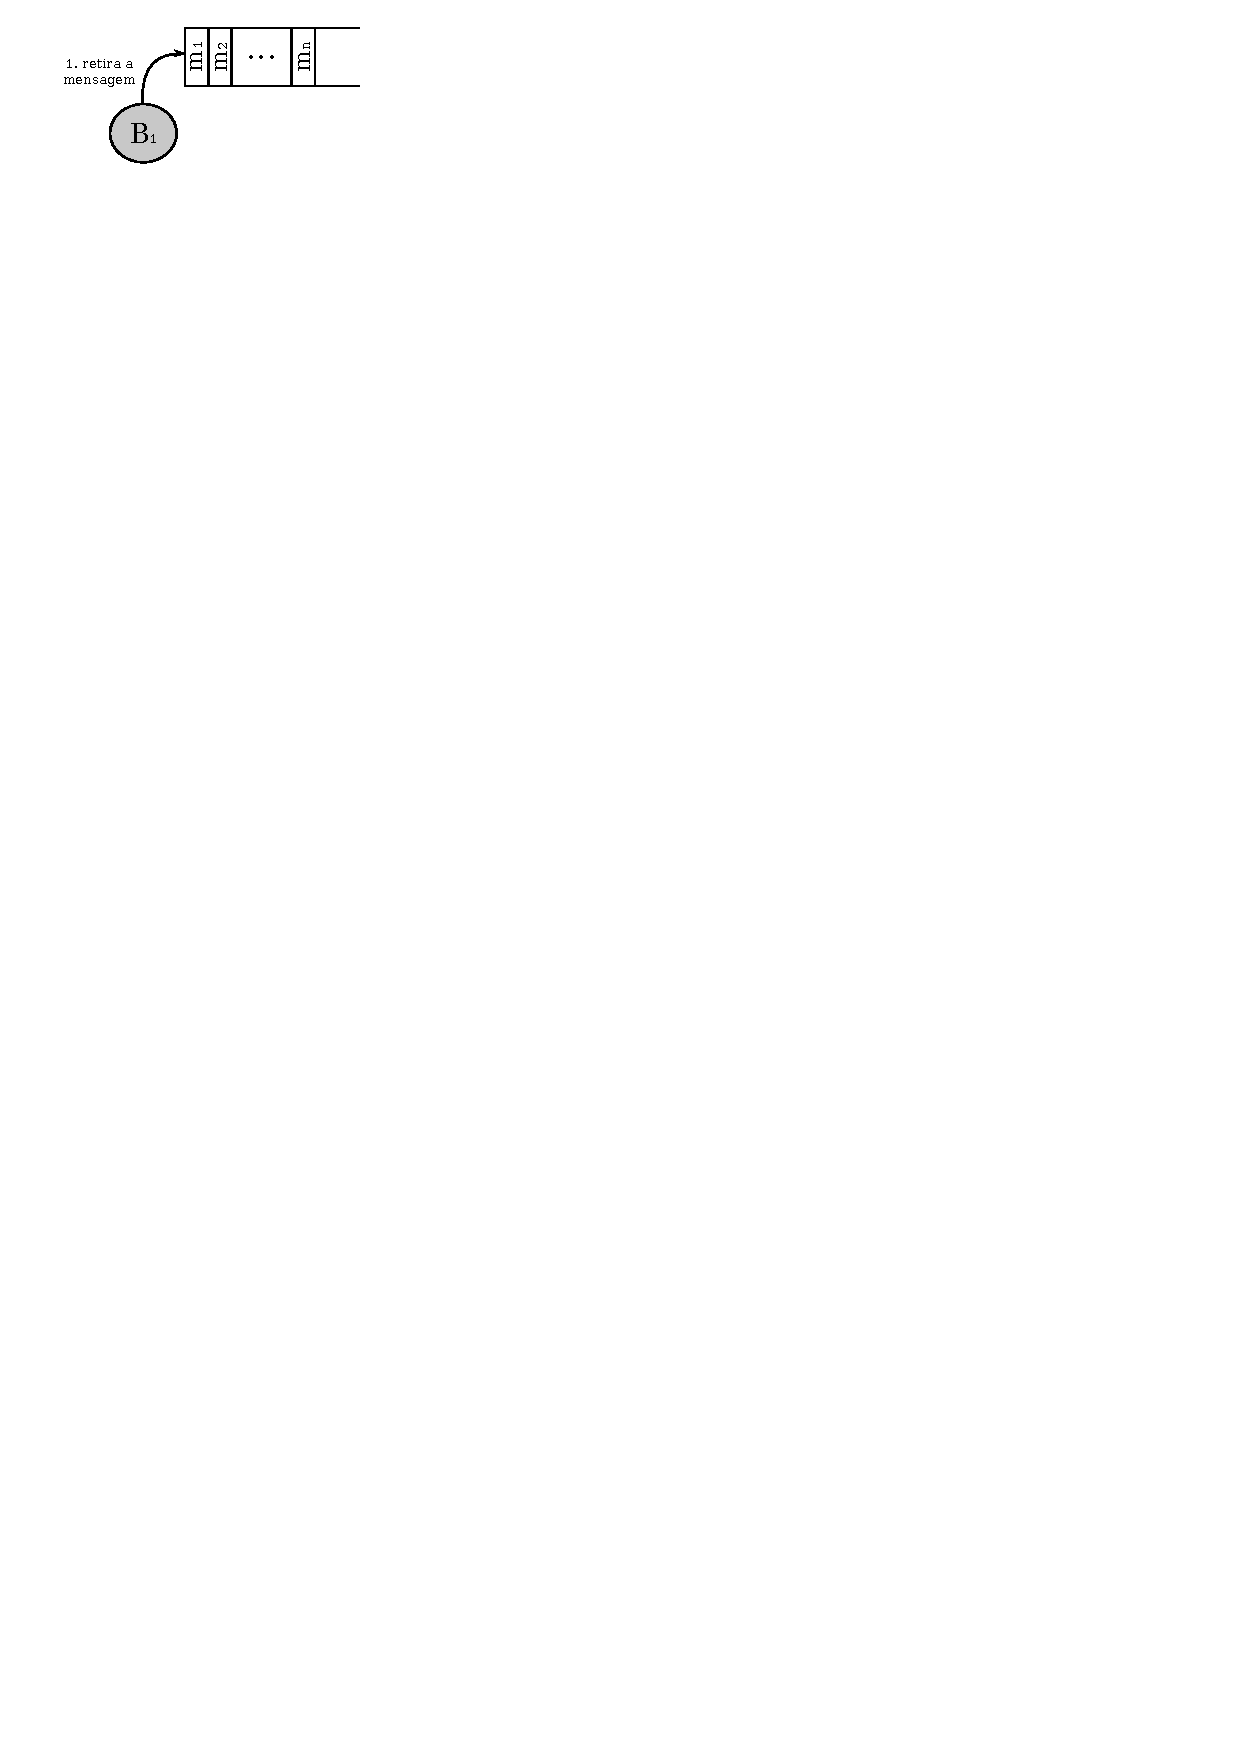
\includegraphics[scale=1.0]{figuras/ator-state-machine0.pdf}
		\end{figure}
 	}
	\only<3>{
 		\begin{figure}[hbtp]
			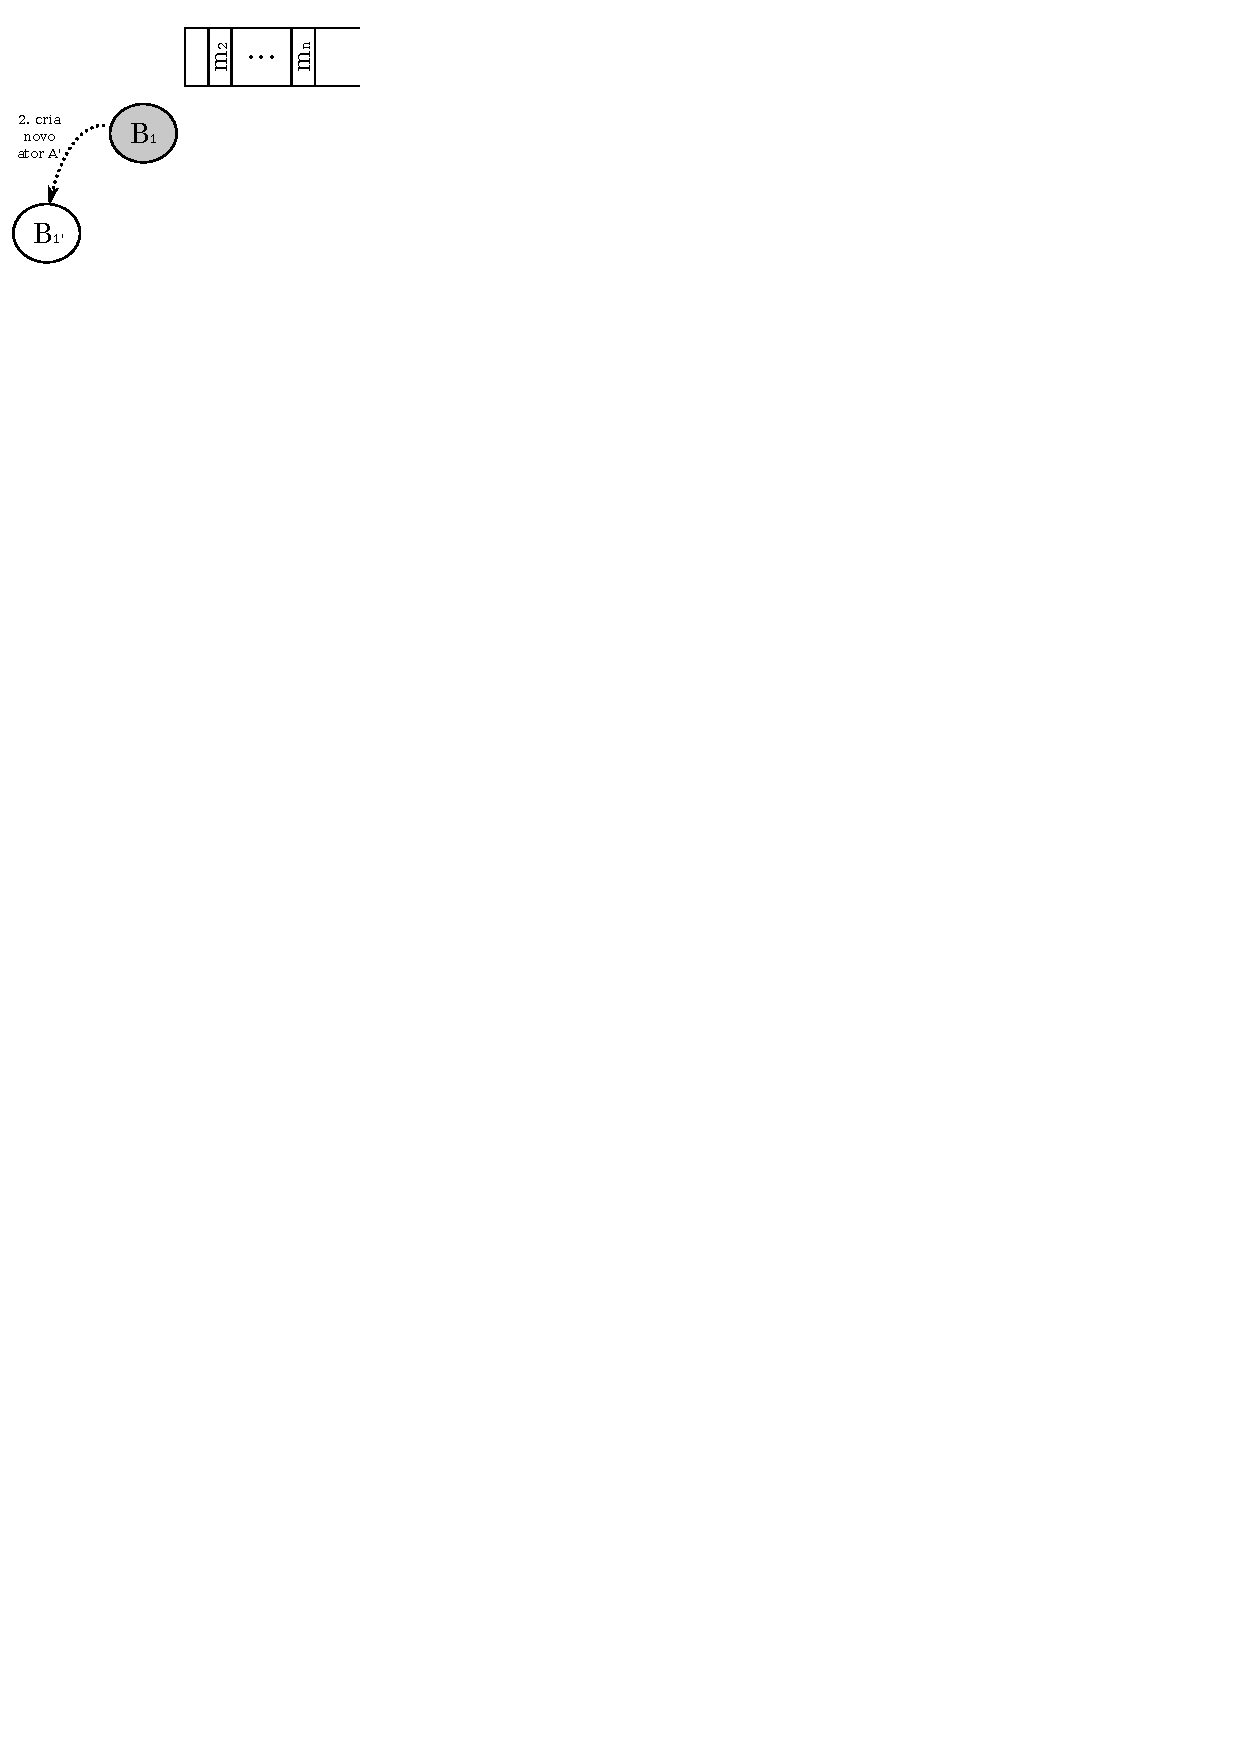
\includegraphics[scale=1.0]{figuras/ator-state-machine1.pdf}
		\end{figure}
 	}	
	\only<4>{
 		\begin{figure}[hbtp]
			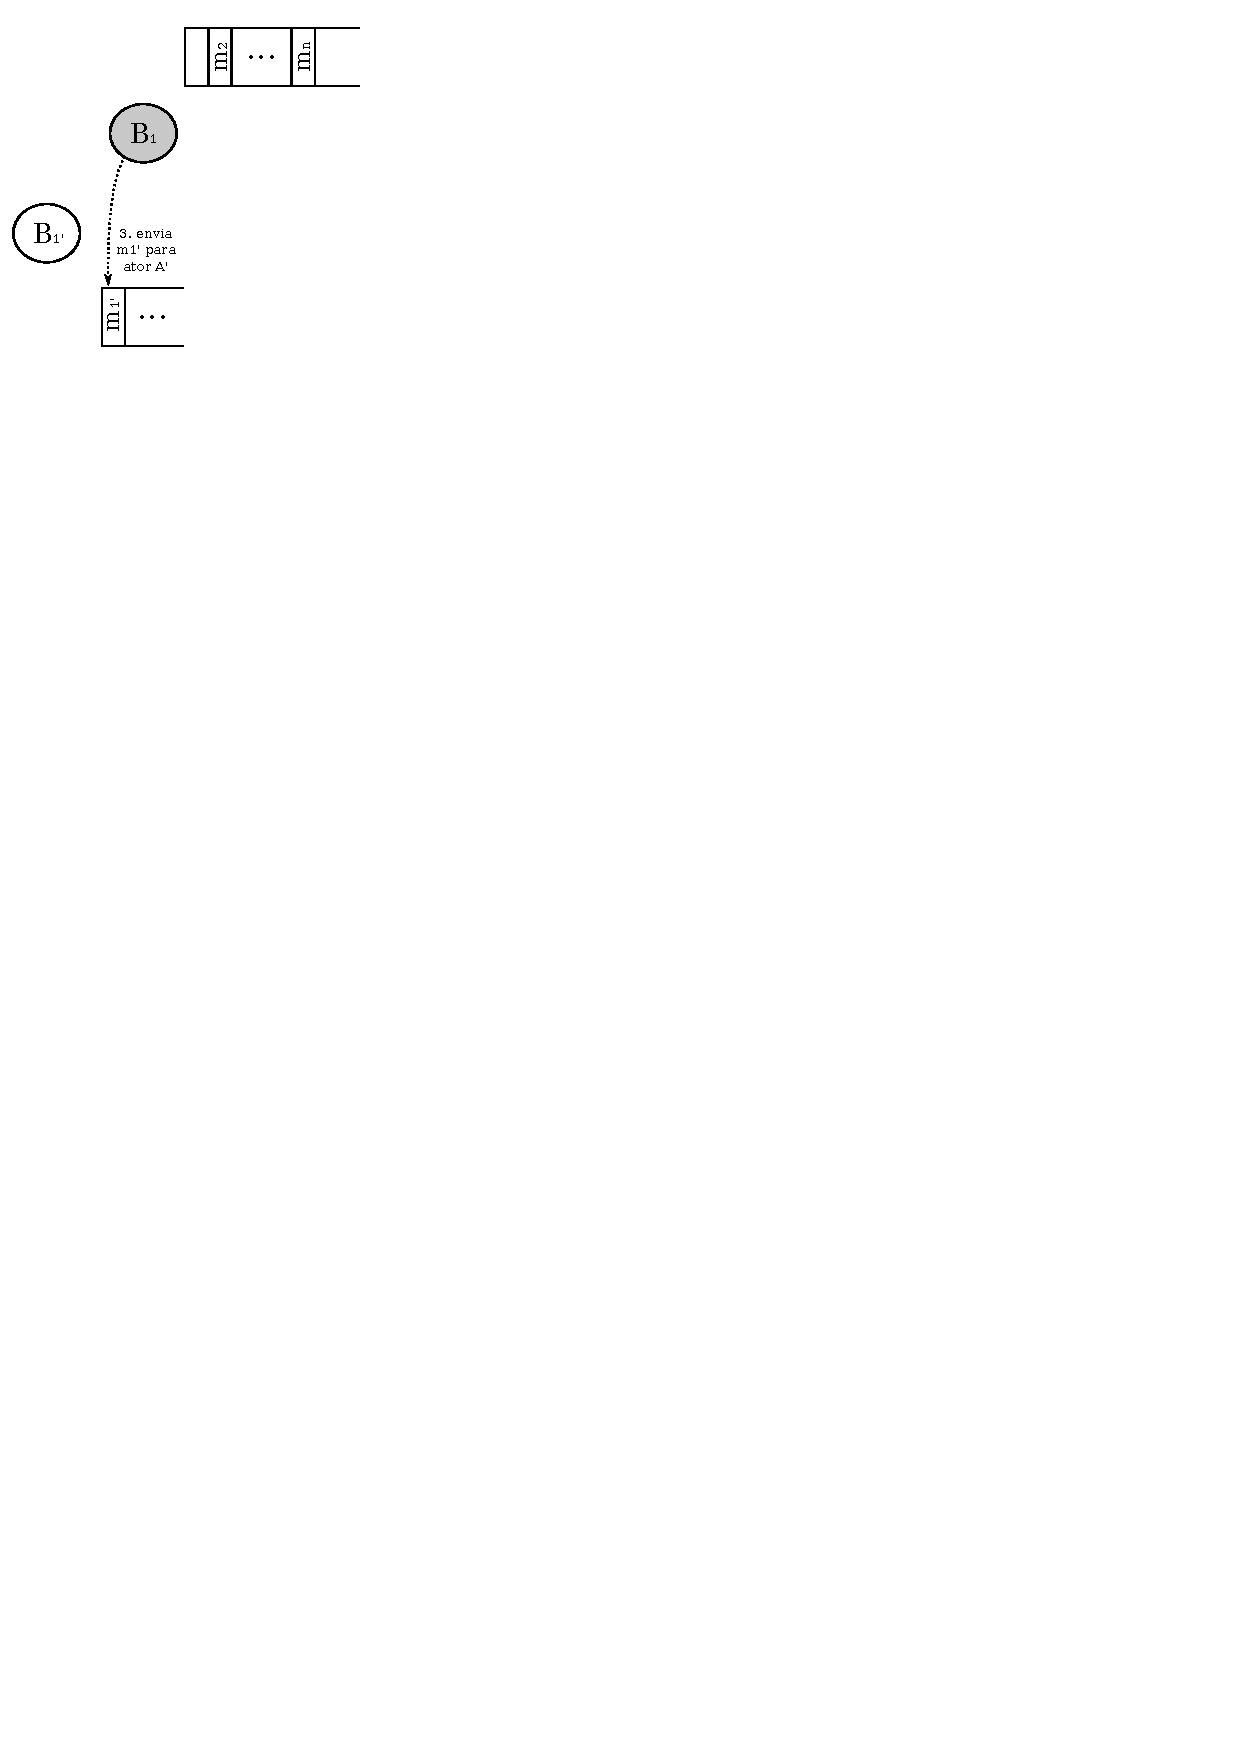
\includegraphics[scale=1.0]{figuras/ator-state-machine3.pdf}
		\end{figure}
 	}
	\only<5>{
 		\begin{figure}[hbtp]
			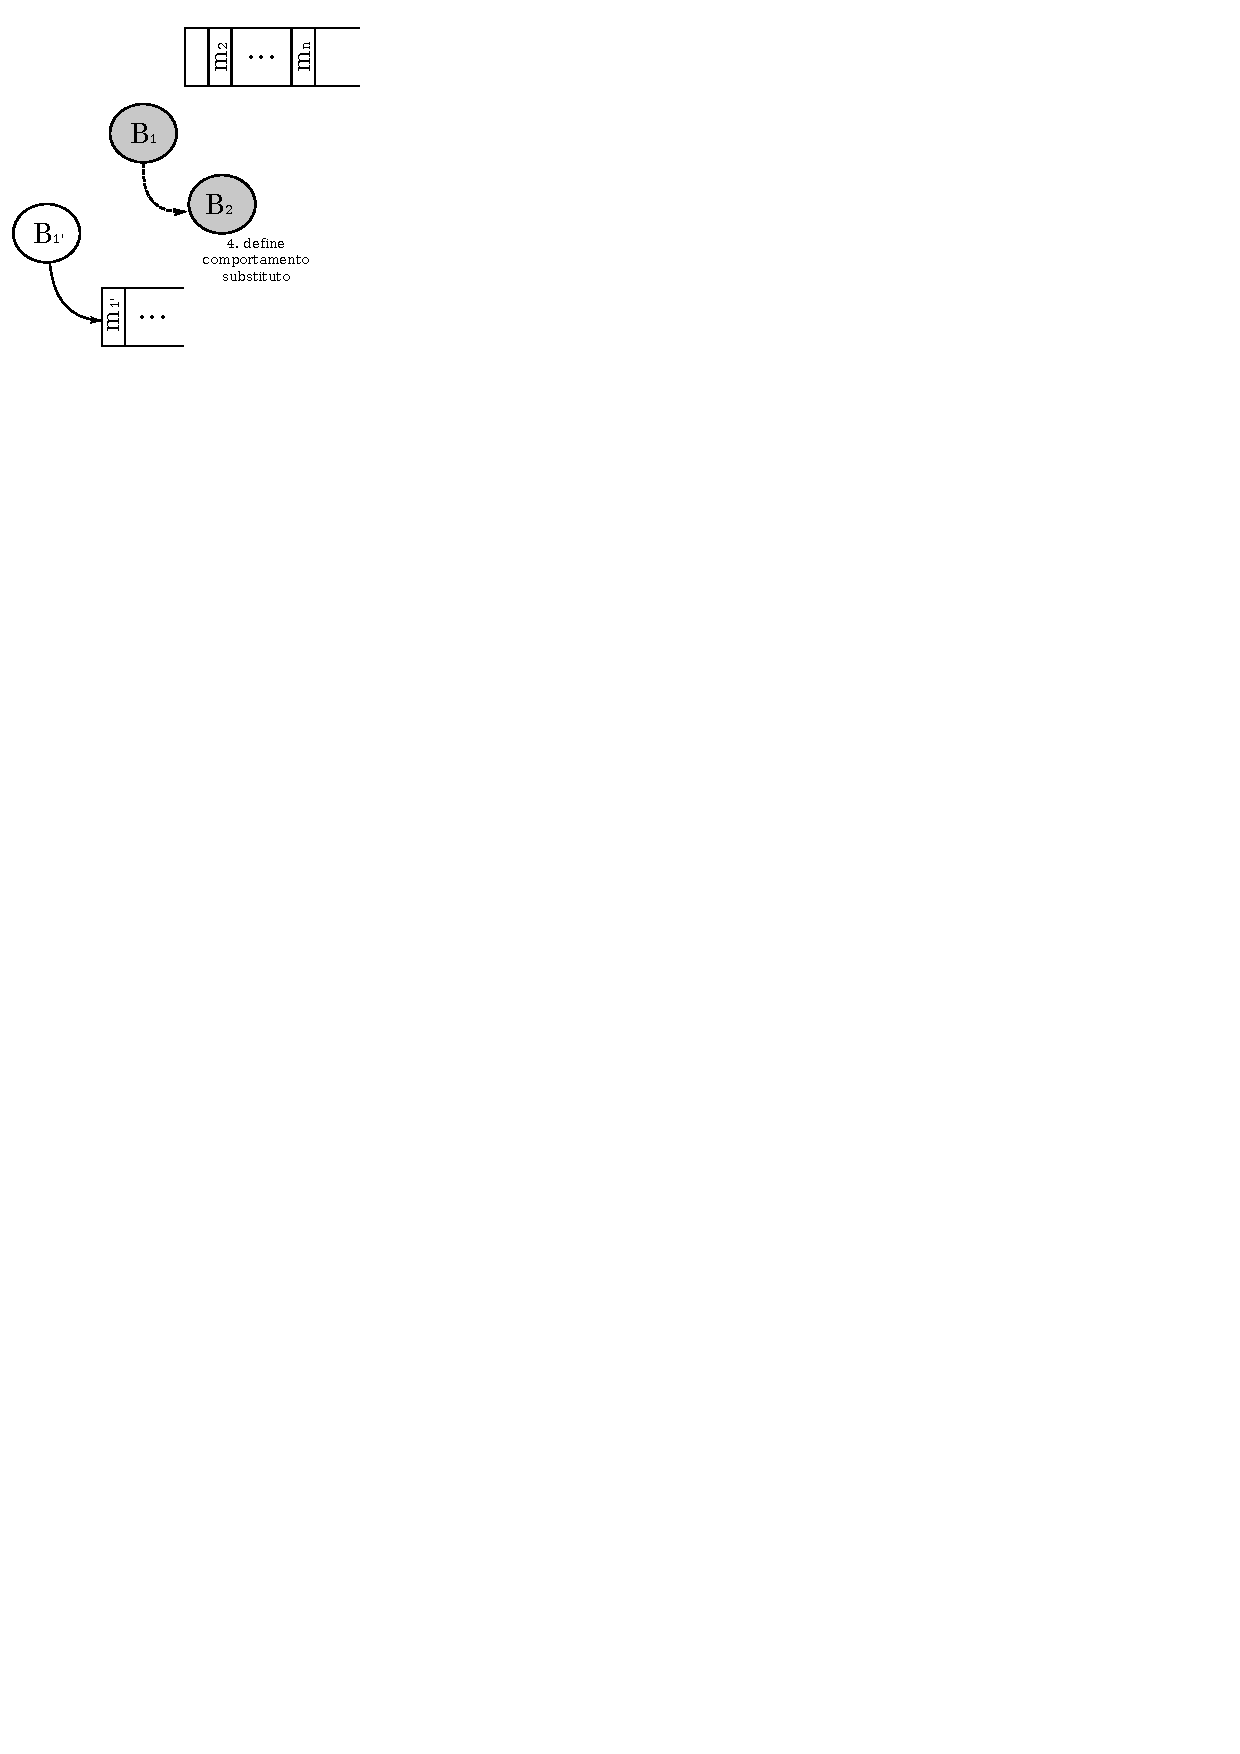
\includegraphics[scale=1.0]{figuras/ator-state-machine4.pdf}
		\end{figure}
	}
	\only<6>{
		\begin{figure}[hbtp]
			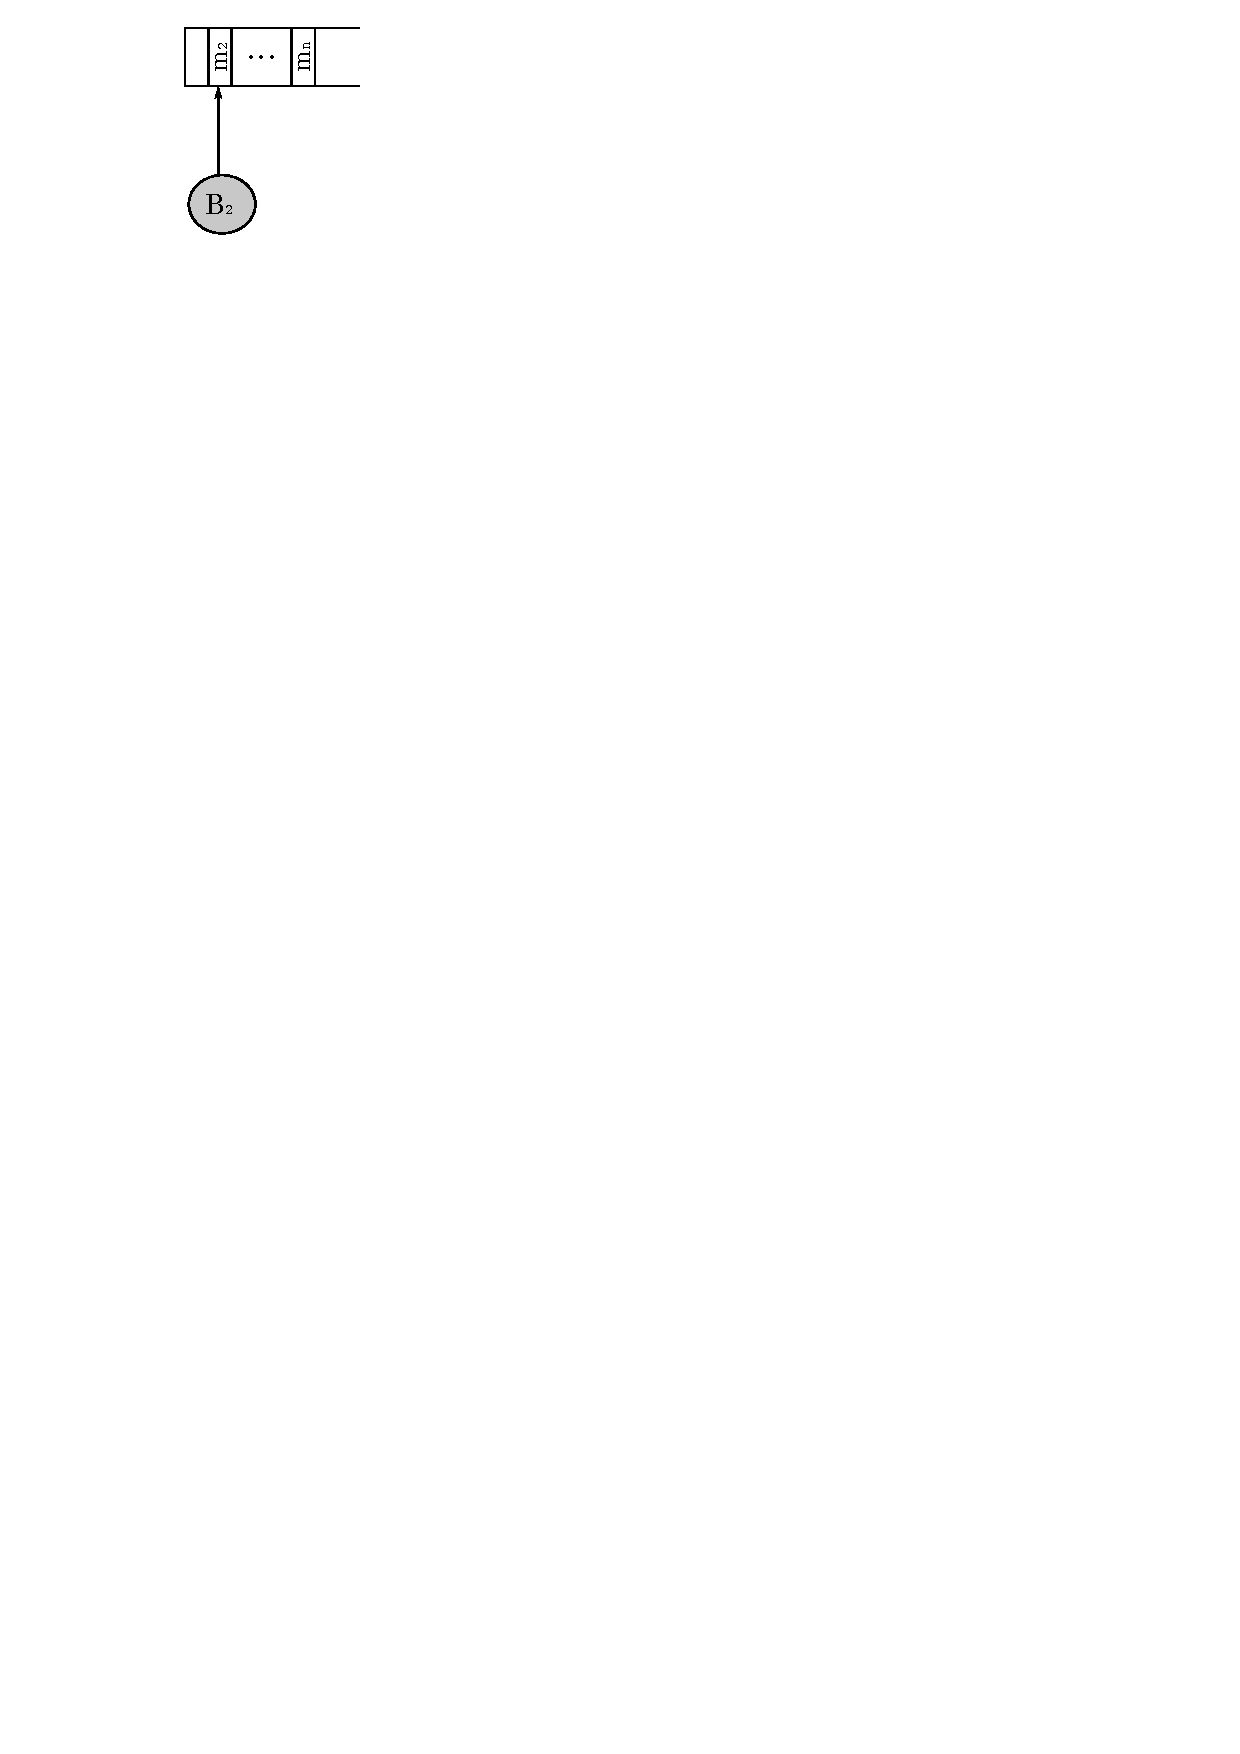
\includegraphics[scale=1.0]{figuras/ator-state-machine5.pdf}
		\end{figure}
	}
	\only<7>{
		Algumas implementa\c{c}\~oes:
			\begin{itemize}
				\item Linguagens: Axum, SALSA e Erlang
				\item C++: Act++, Thal e Theron
				\item Smalltalk: Actalk
				\item Python: Parley e Stackless Python
				\item Ruby: Stage e Rubinius
				\item .Net: Asynchronous Agent Library e Retlang
				\item Java: Akka, Kilim, Jetlang e Actor Foundry
				\item Scala: Scala Actors, Akka e Scalaz
			\end{itemize}
 	}
}

\subsection{Advanced Message Queuing Protocol}
\frame{
\frametitle{Advanced Message Queuing Protocol}
	\only<1>{
 		\note{
 			\begin{itemize}
				\item Protocolo aberto desenvolvido por um conjunto de empresas com o objetivo de padroniza\c{c}\~ao
			          e redu\c{c}\~ao de custos na integra\c{c}\~ao de sistemas
				\item Al\'em da defini\c{c}\~ao do protocolo, define tamb\'em a sem\^antica dos servi\c{c}os de trocas de mensagens 
				\item Objetiva que as capacidades de MOMs estejam dispon\'iveis pervasivamente nas empresas
			\end{itemize}
		}
		\begin{figure}[hbtp]
			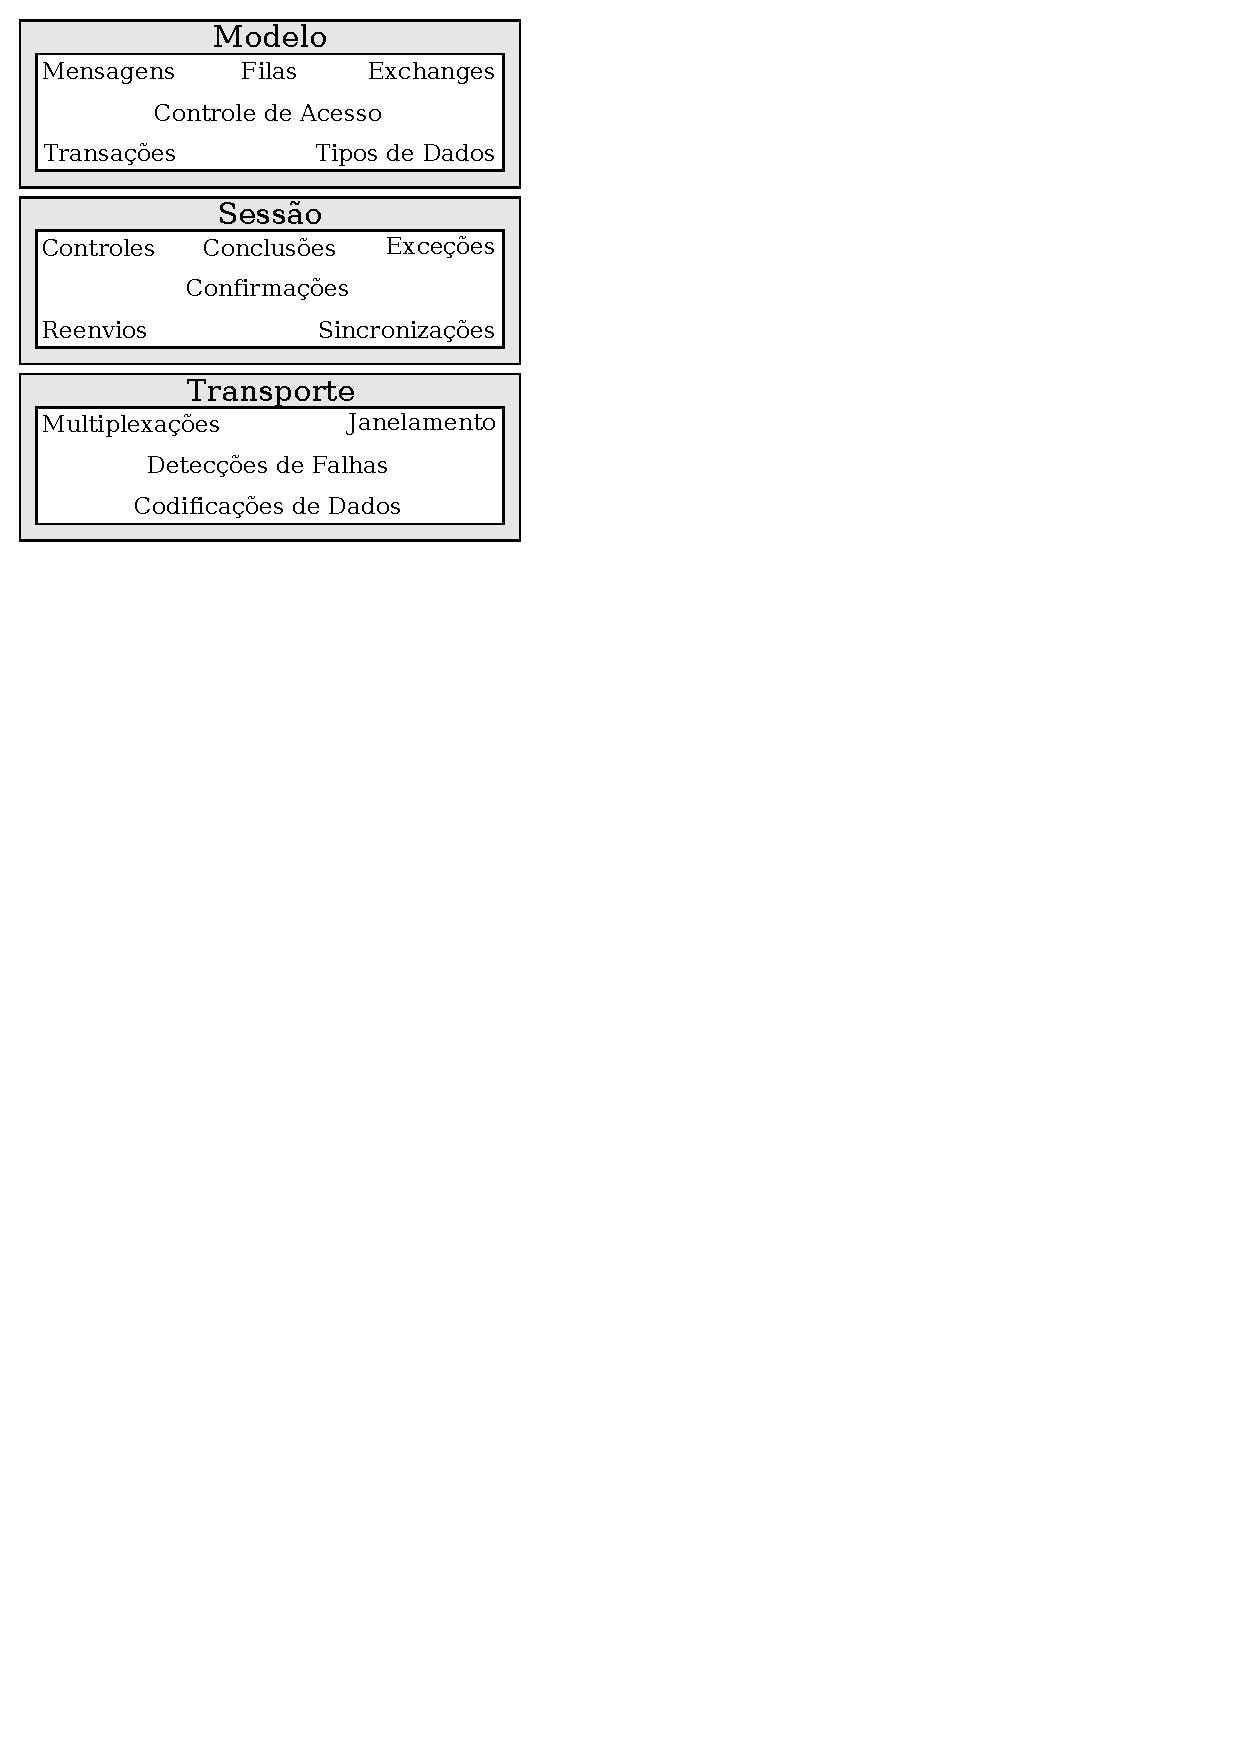
\includegraphics[scale=.60]{figuras/protocol_overview.pdf}
		\end{figure}
	}
	\only<2>{
 		\note{
 			Para nao esquecer: comentar brevemente quem eh quem antes (adicionar outras notas) 
			comentar tamb�m de propriedades como transiente, persistente e auto_delete.					
	 		Analogia com sistemas de \textit{email}:
	 		\begin{itemize}
				\item Mensagens AMQP s\~ao an\'alogas a mensagens de correio eletr\^onico
				\item Filas s\~ao an\'alogas a caixas de correio
				\item \textit{Exchanges} s\~ao an\'alogas a agentes de transfer\^encia de mensagens (MTA).
				 Com base nas chaves de roteamento (To, Cc e Bcc no caso de correio eletr\^onico), eles verificam
				as tabelas de registro e decidem como enviar as mensagens para uma ou mais caixas de correio
				\item \textit{Bindings} correspondem a entradas nas tabelas de roteamento do MTA		
			\end{itemize}
 		}
		\begin{figure}[hbtp]
			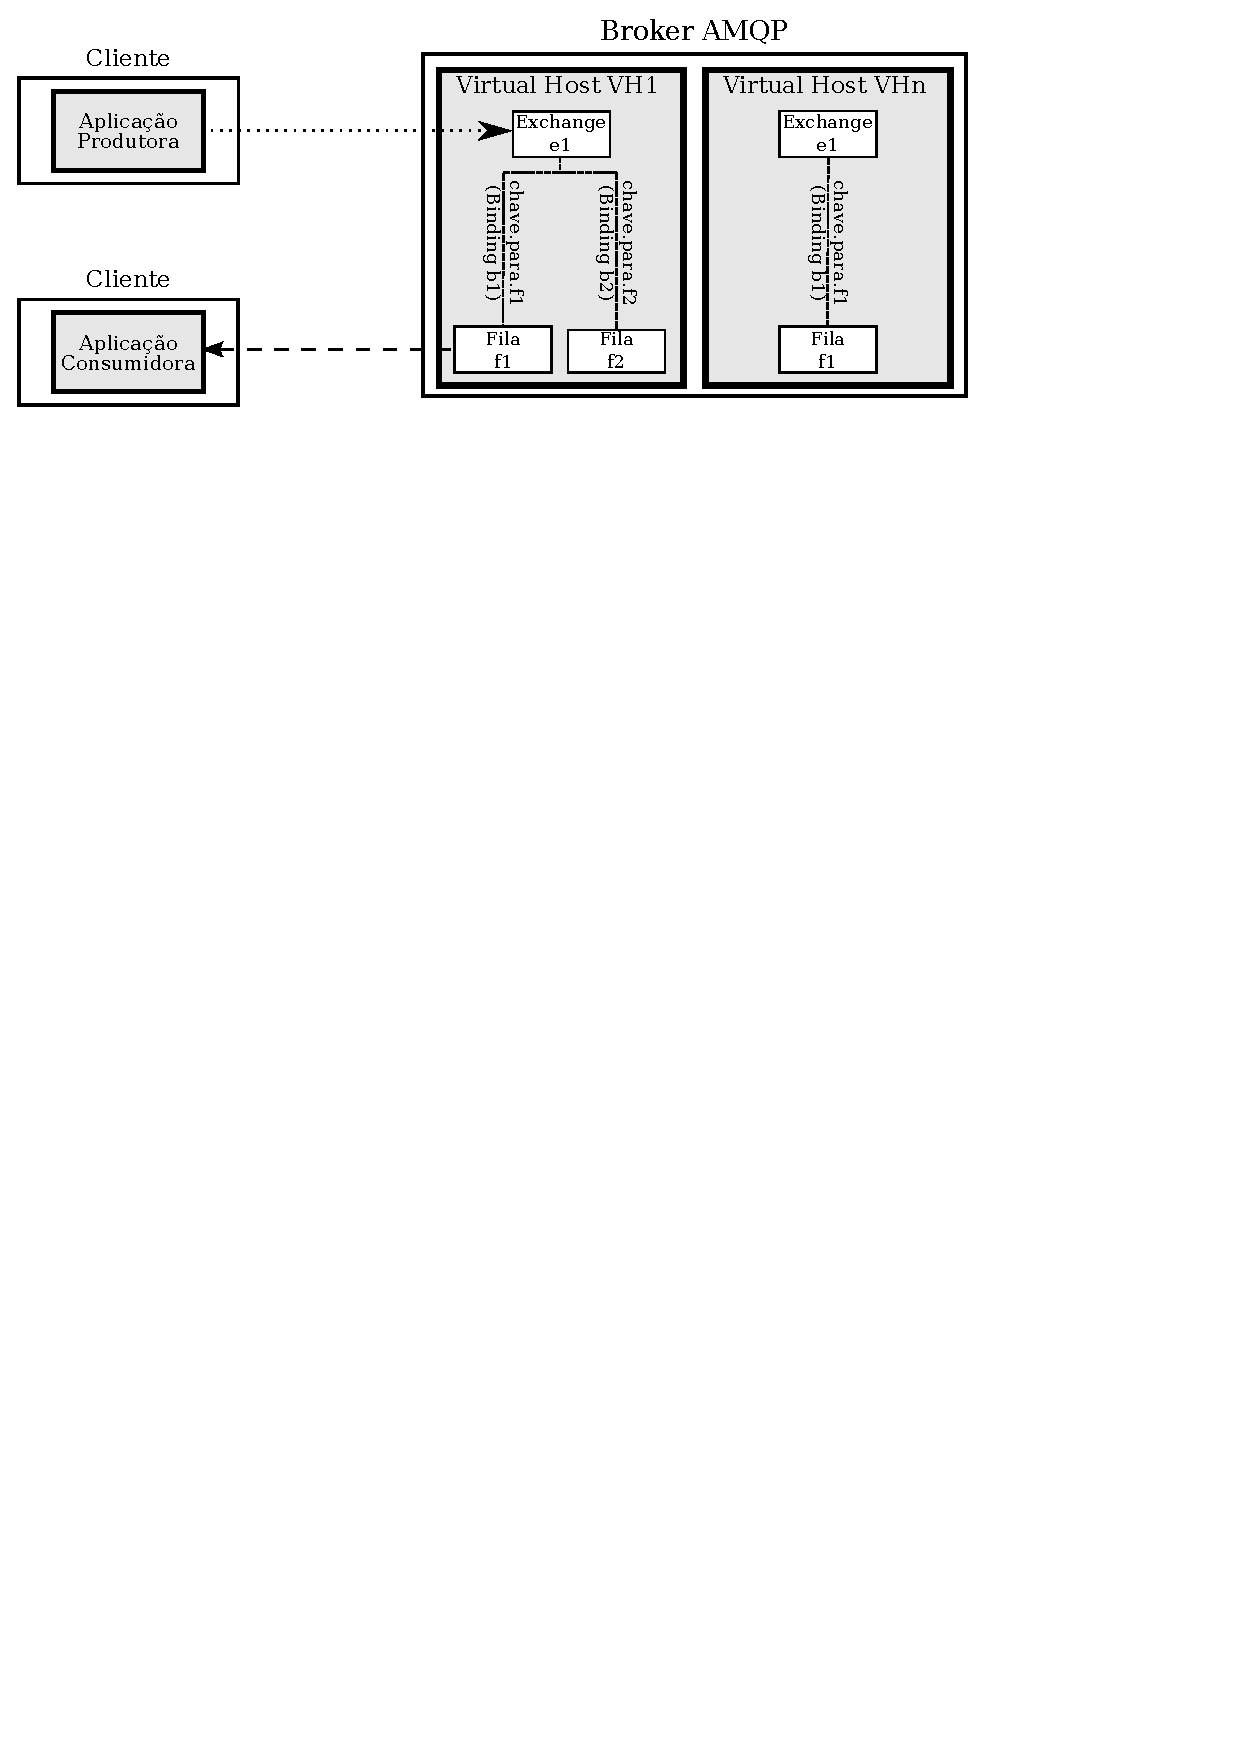
\includegraphics[scale=.70]{figuras/amqp-overview-slides.pdf}
		\end{figure}
	}	
 	\only<3>{ 		
  		\begin{figure}[hbtp]
			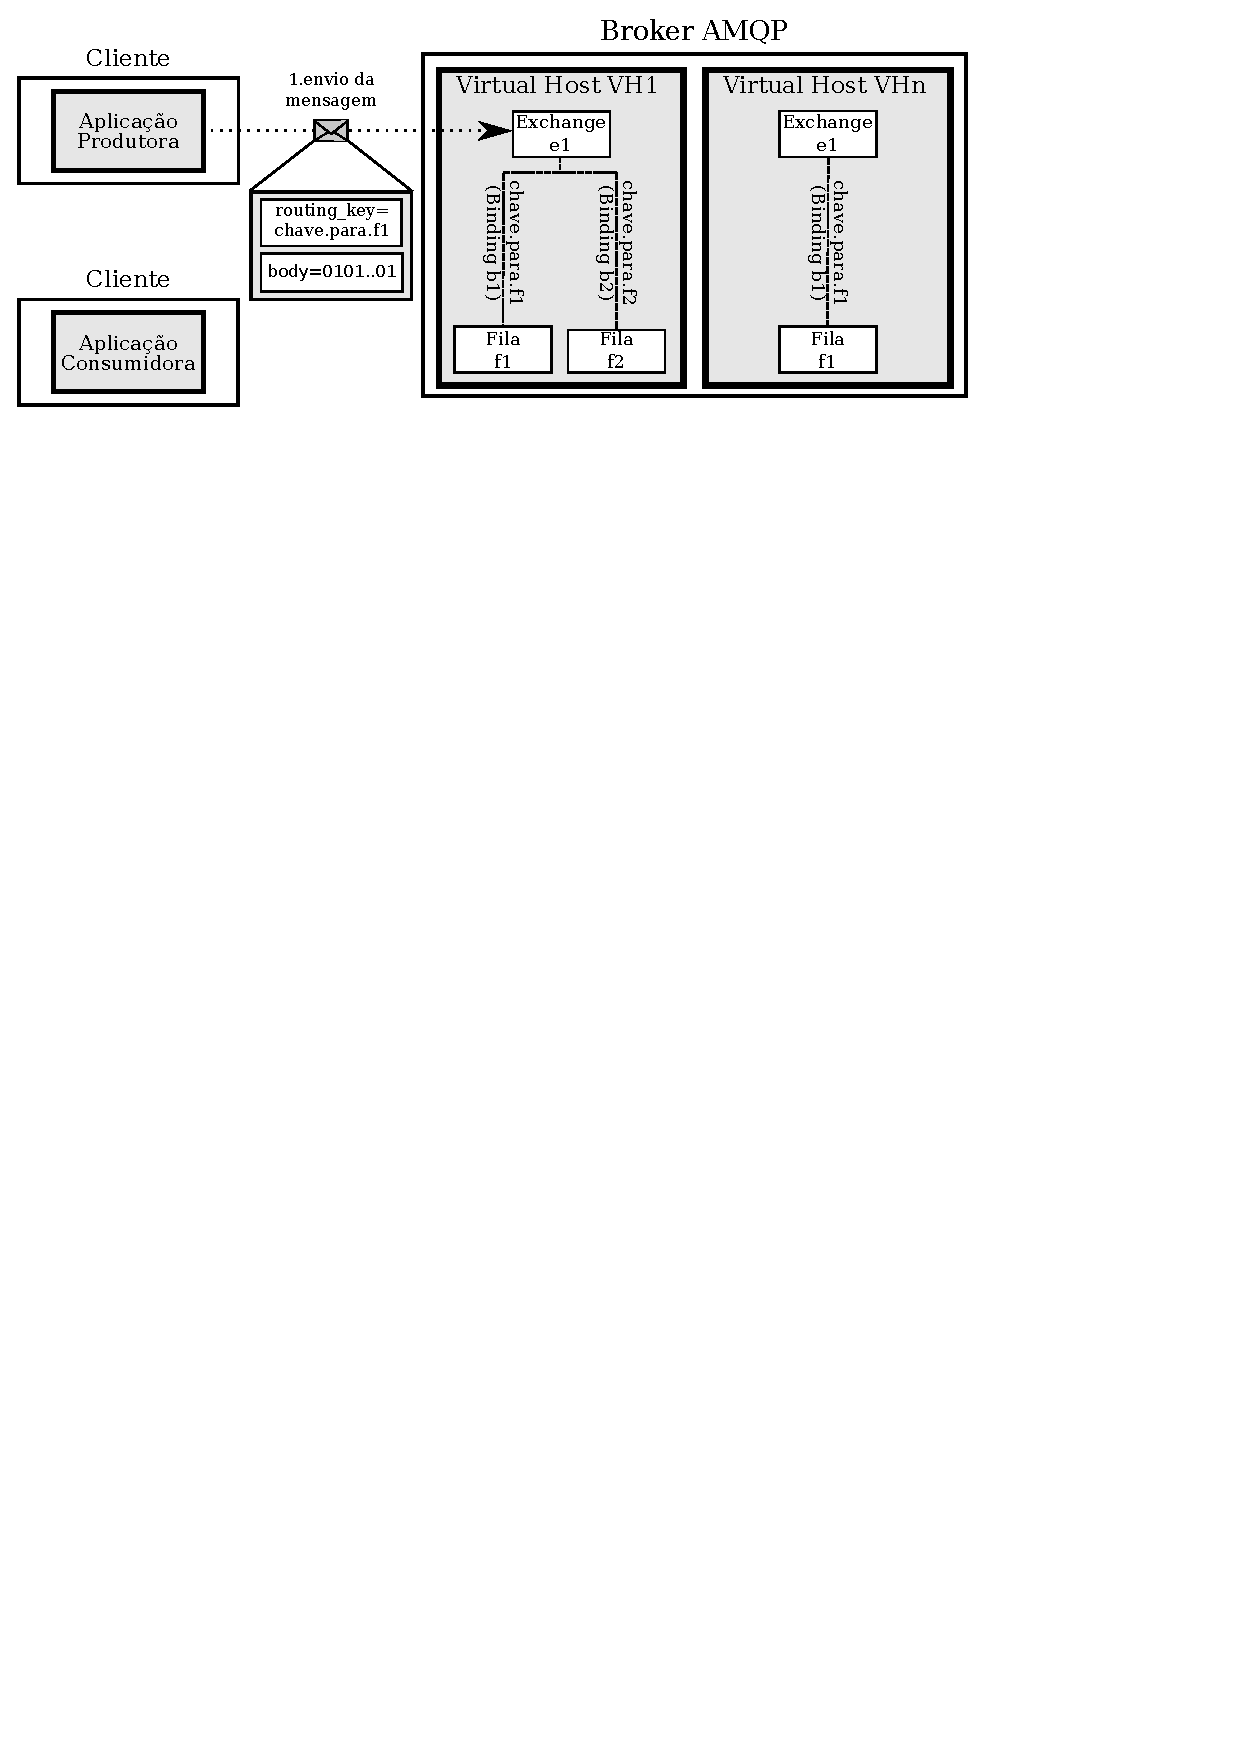
\includegraphics[scale=.70]{figuras/amqp-message-flow0.pdf}
		\end{figure}
 	}
 	\only<4>{ 		
  		\begin{figure}[hbtp]
			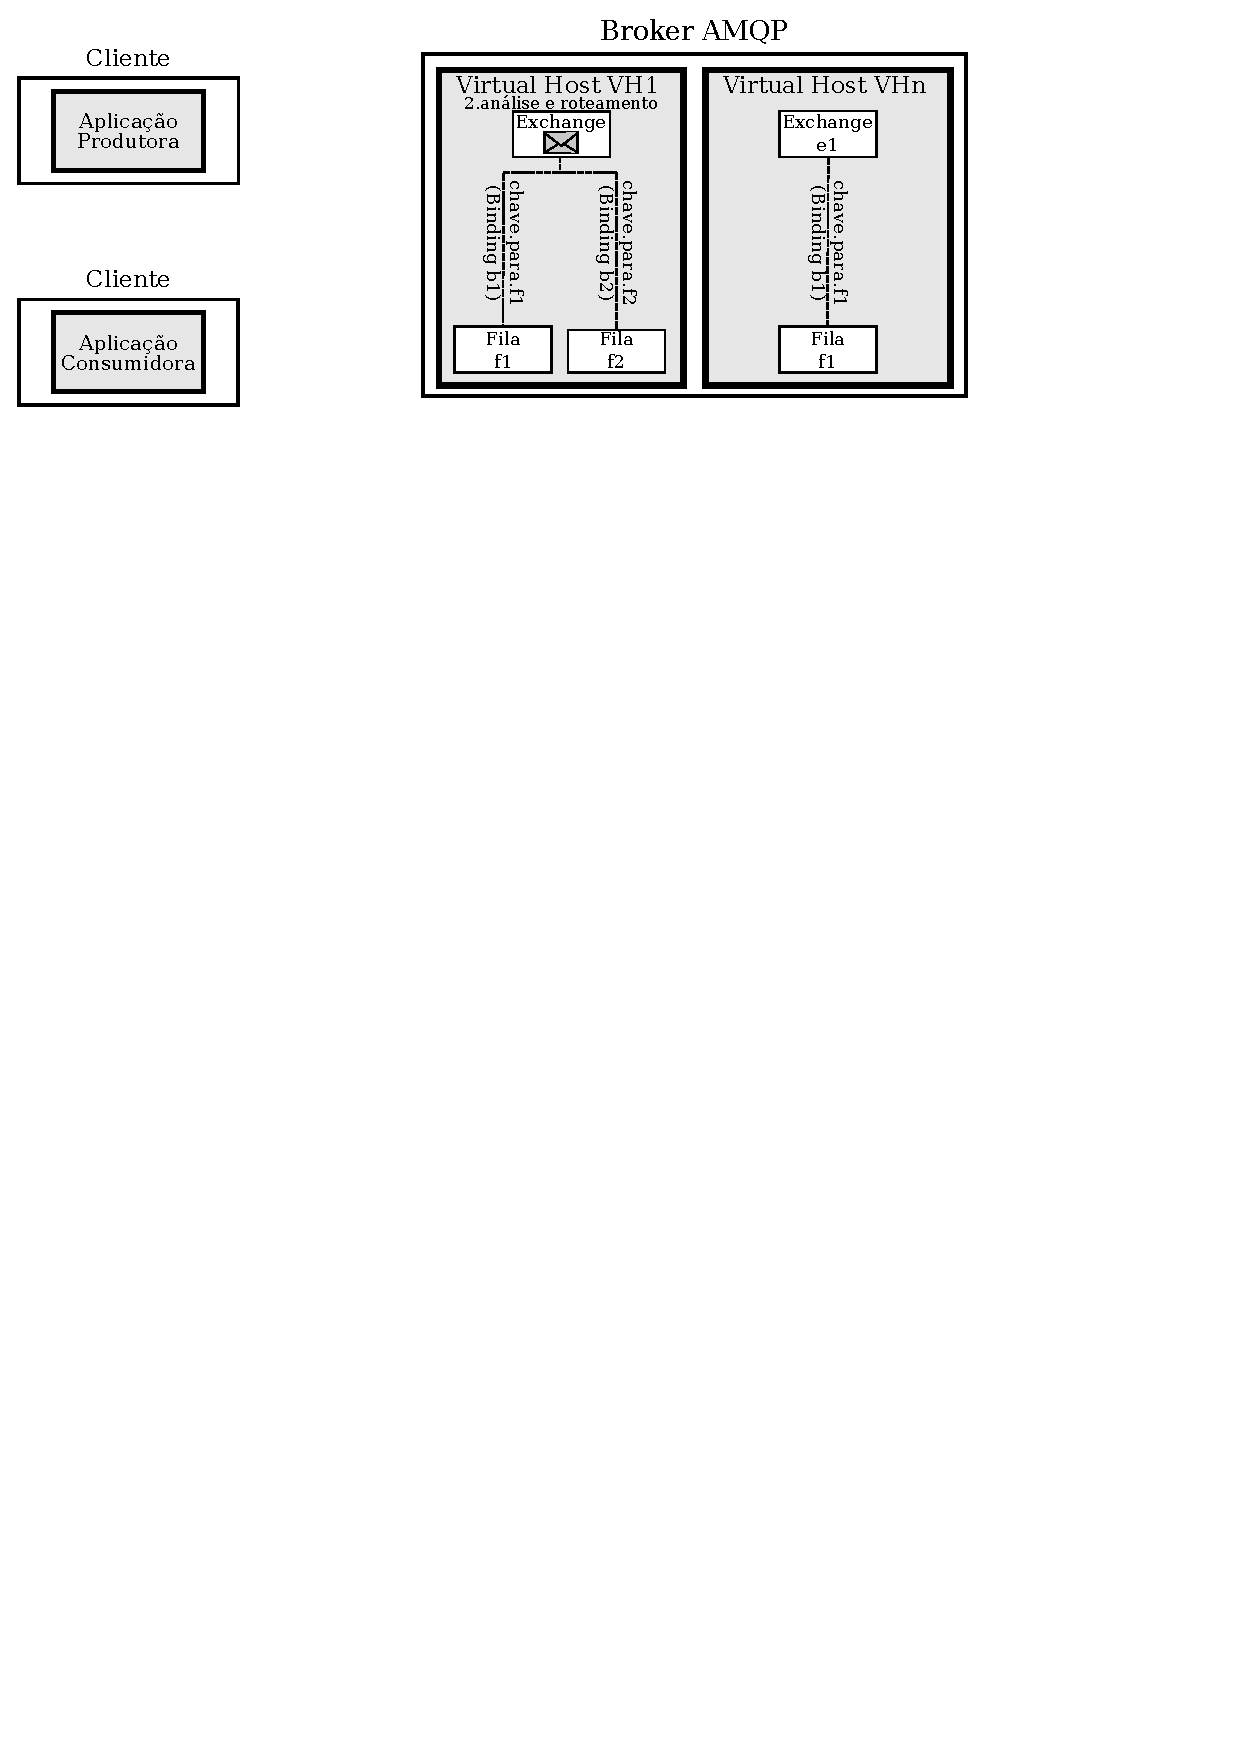
\includegraphics[scale=.70]{figuras/amqp-message-flow1.pdf}
		\end{figure}
 	}
 	\only<5>{ 		
  		\begin{figure}[hbtp]
			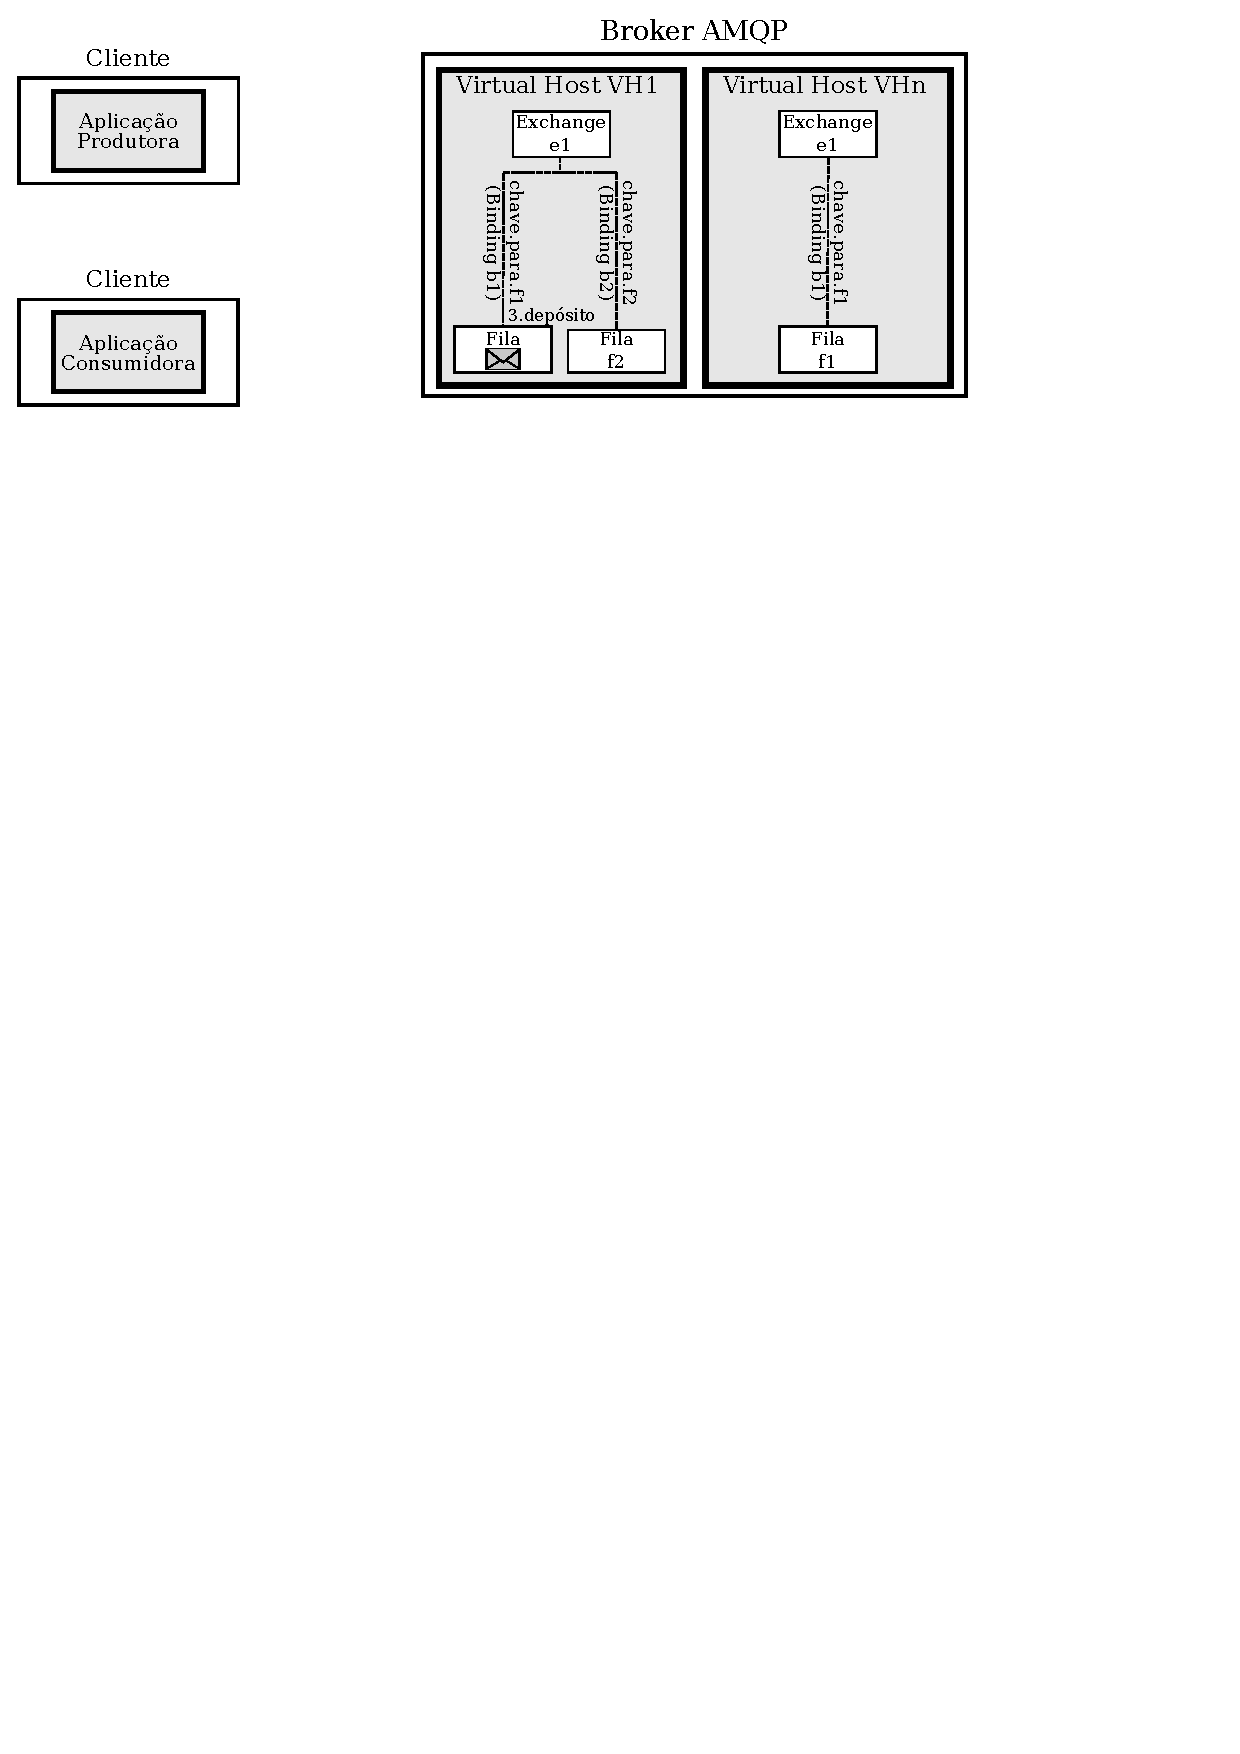
\includegraphics[scale=.70]{figuras/amqp-message-flow2.pdf}
		\end{figure}
 	}
 	\only<6>{ 		
  		\begin{figure}[hbtp]
			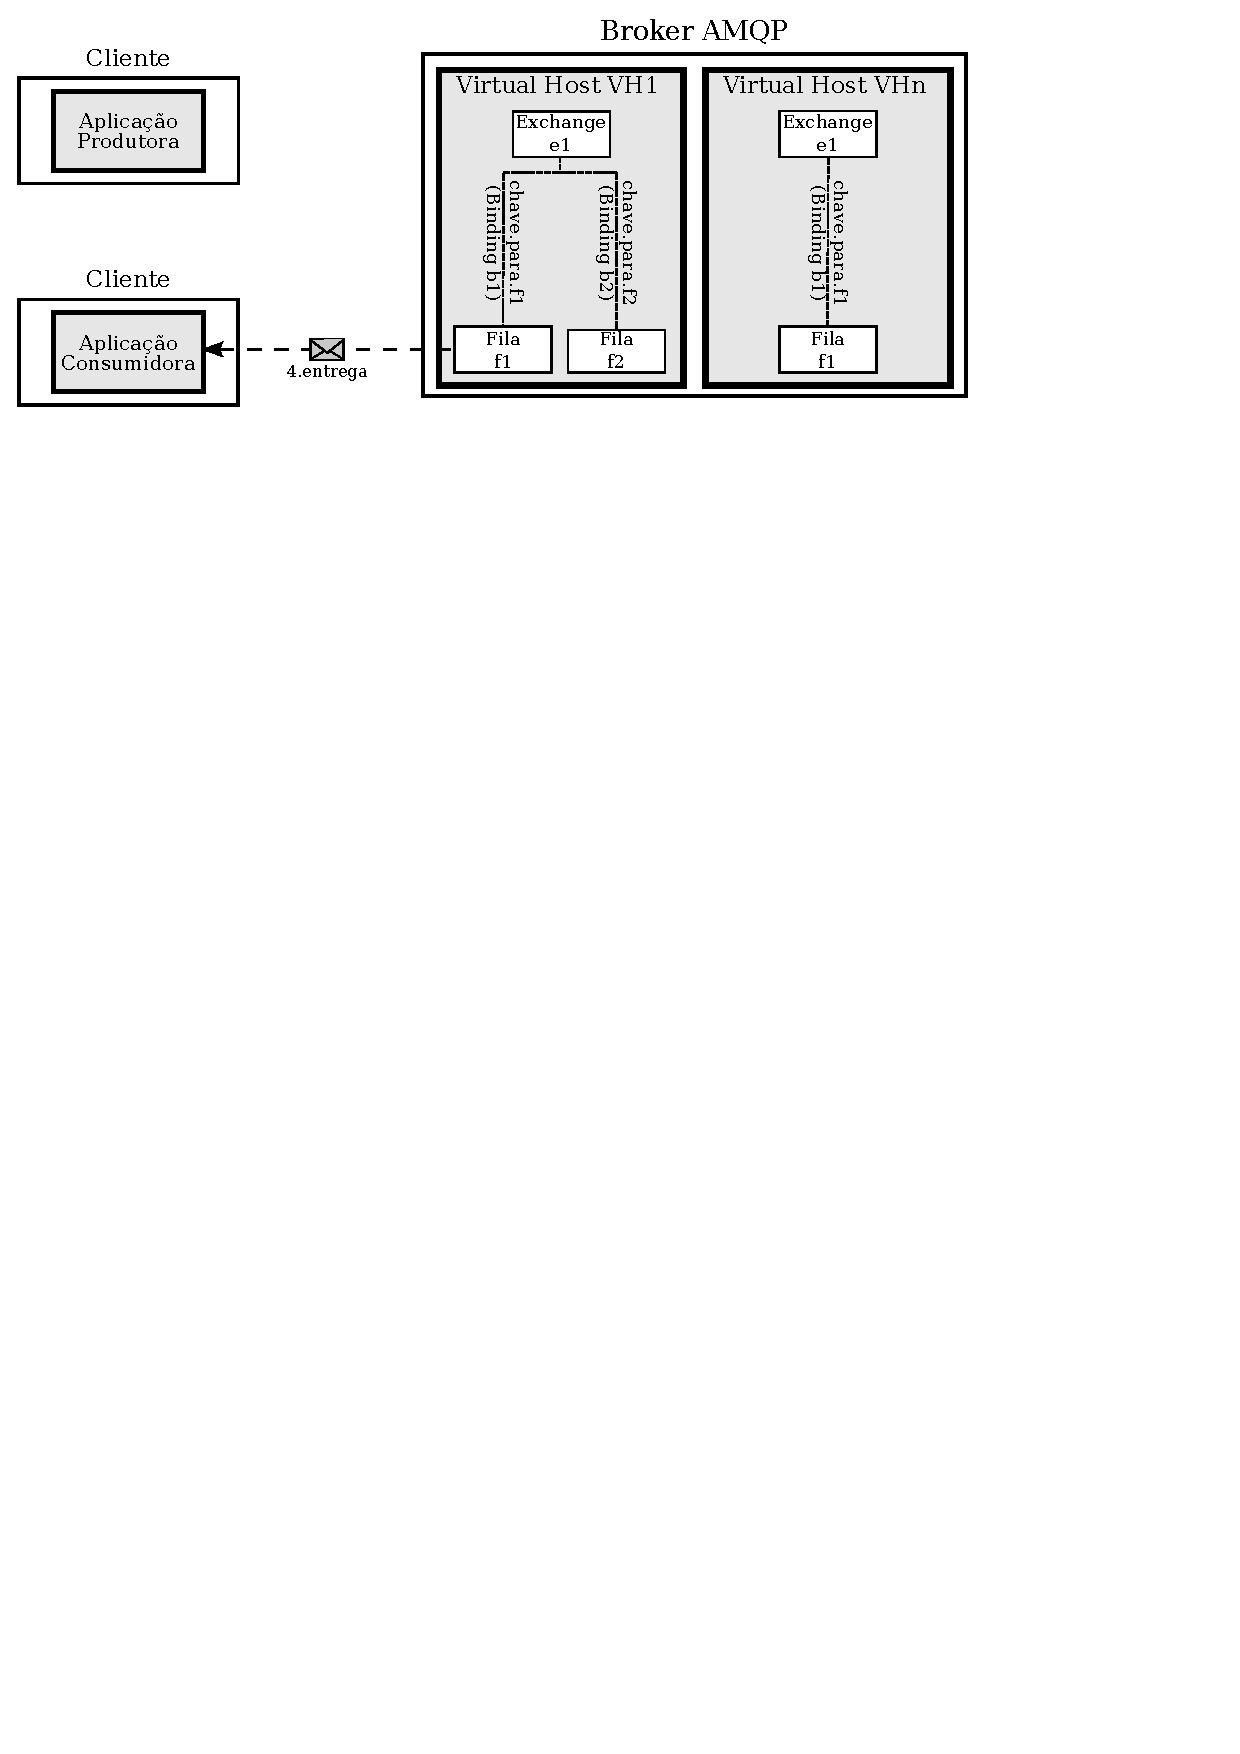
\includegraphics[scale=.70]{figuras/amqp-message-flow3.pdf}
		\end{figure}
 	}
	
	\only<7>{
 		Algumas implementa\c{c}\~oes:
		\begin{itemize}
			\item Apache Qpid
			\item ZeroMQ
			\item RabbitMQ
		\end{itemize}

		\vspace{0.2in}
 		Utilizamos neste trabalho a implementa\c{c}\~ao de c\'odigo aberto RabbitMQ
 	}
}
\section{Atores no projeto Akka} 
\frame{\frametitle{Atores no projeto Akka}
	\note{lembrar que ator remoto eh sinonimo de ator remotamente acessivel.}
	O projeto Akka disponibiliza dois tipos de atores:
	\begin{enumerate}
		\item Atores locais: um ator local \'e um ator que pode receber mensagens apenas de atores residentes na mesma m\'aquina virtual
		\item Atores remotos: um ator remoto \'e um ator que pode receber mensagens de quaisquer outros atores, inclusive daqueles residentes
		em outras m\'aquinas virtuais
	\end{enumerate}
}
\subsection{Atores locais}
\begin{frame}[fragile]{Atores locais}

	\note{comentar sobre o envio assincrono, e que theActor na verdade eh uma ActorRef - LocalActorRef. e do self}
	Declara\c{c}\~ao e uso de um ator:
		\begin{lstlisting}[frame=tb]
class SampleActor(val name: String) extends akka.actor.Actor {
  def this() = this("No name")
  
  def receive = {
    case "hello" => println("%s received hello".format(name))
    case  _ => println("%s received unknown".format(name))
  }
}

/*  theActor representa uma LocalActorRef  */
val theActor = Actor.actorOf[SampleActor].start
theActor ! "hello" 
		\end{lstlisting}
\end{frame}
\frame{\frametitle{Envios ass\'incronos e sem resposta -- !}
	\note{comentar dos tipos de despachadores}
	\only<1>{ 		
  		\begin{figure}[hbtp]
			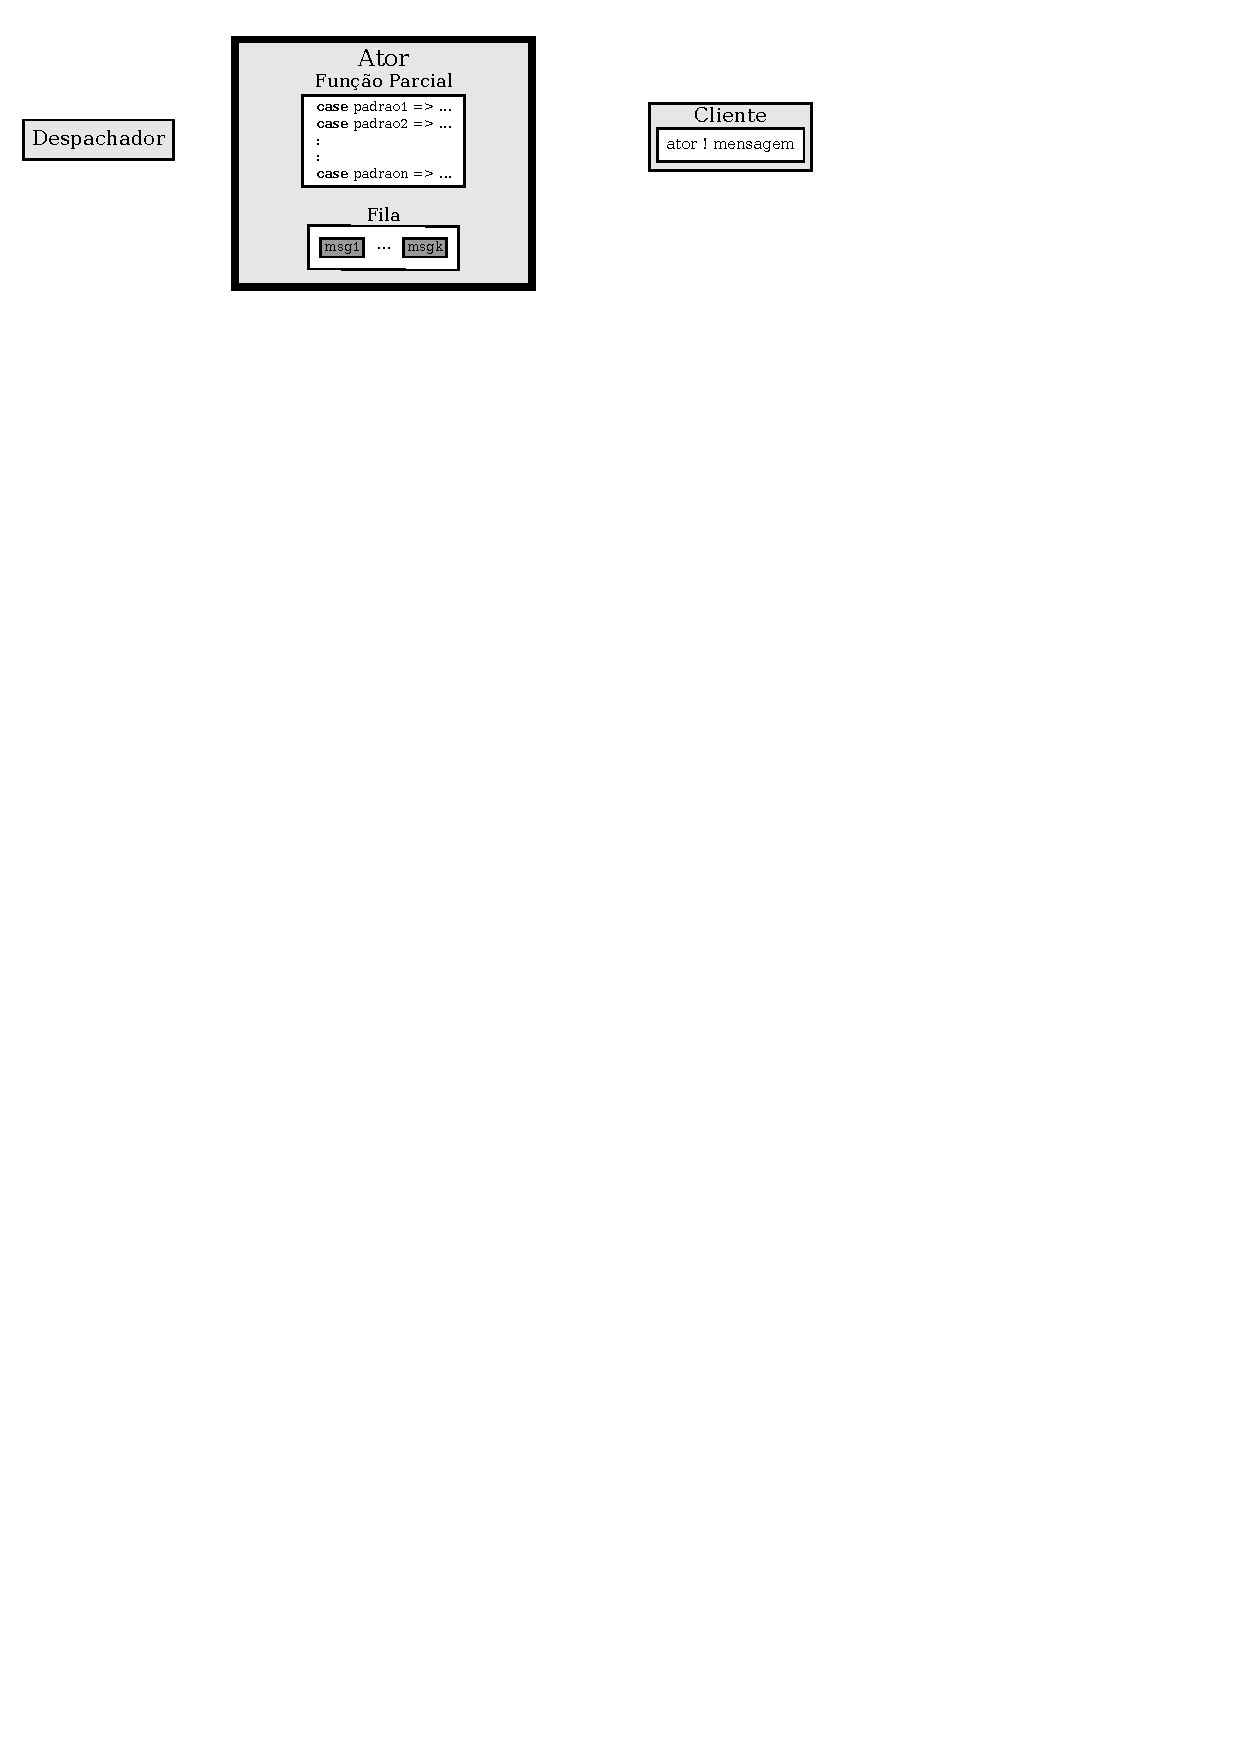
\includegraphics[scale=.70]{figuras/local-actor-message0.pdf}
		\end{figure}
 	}
	\only<2>{ 		
  		\begin{figure}[hbtp]
			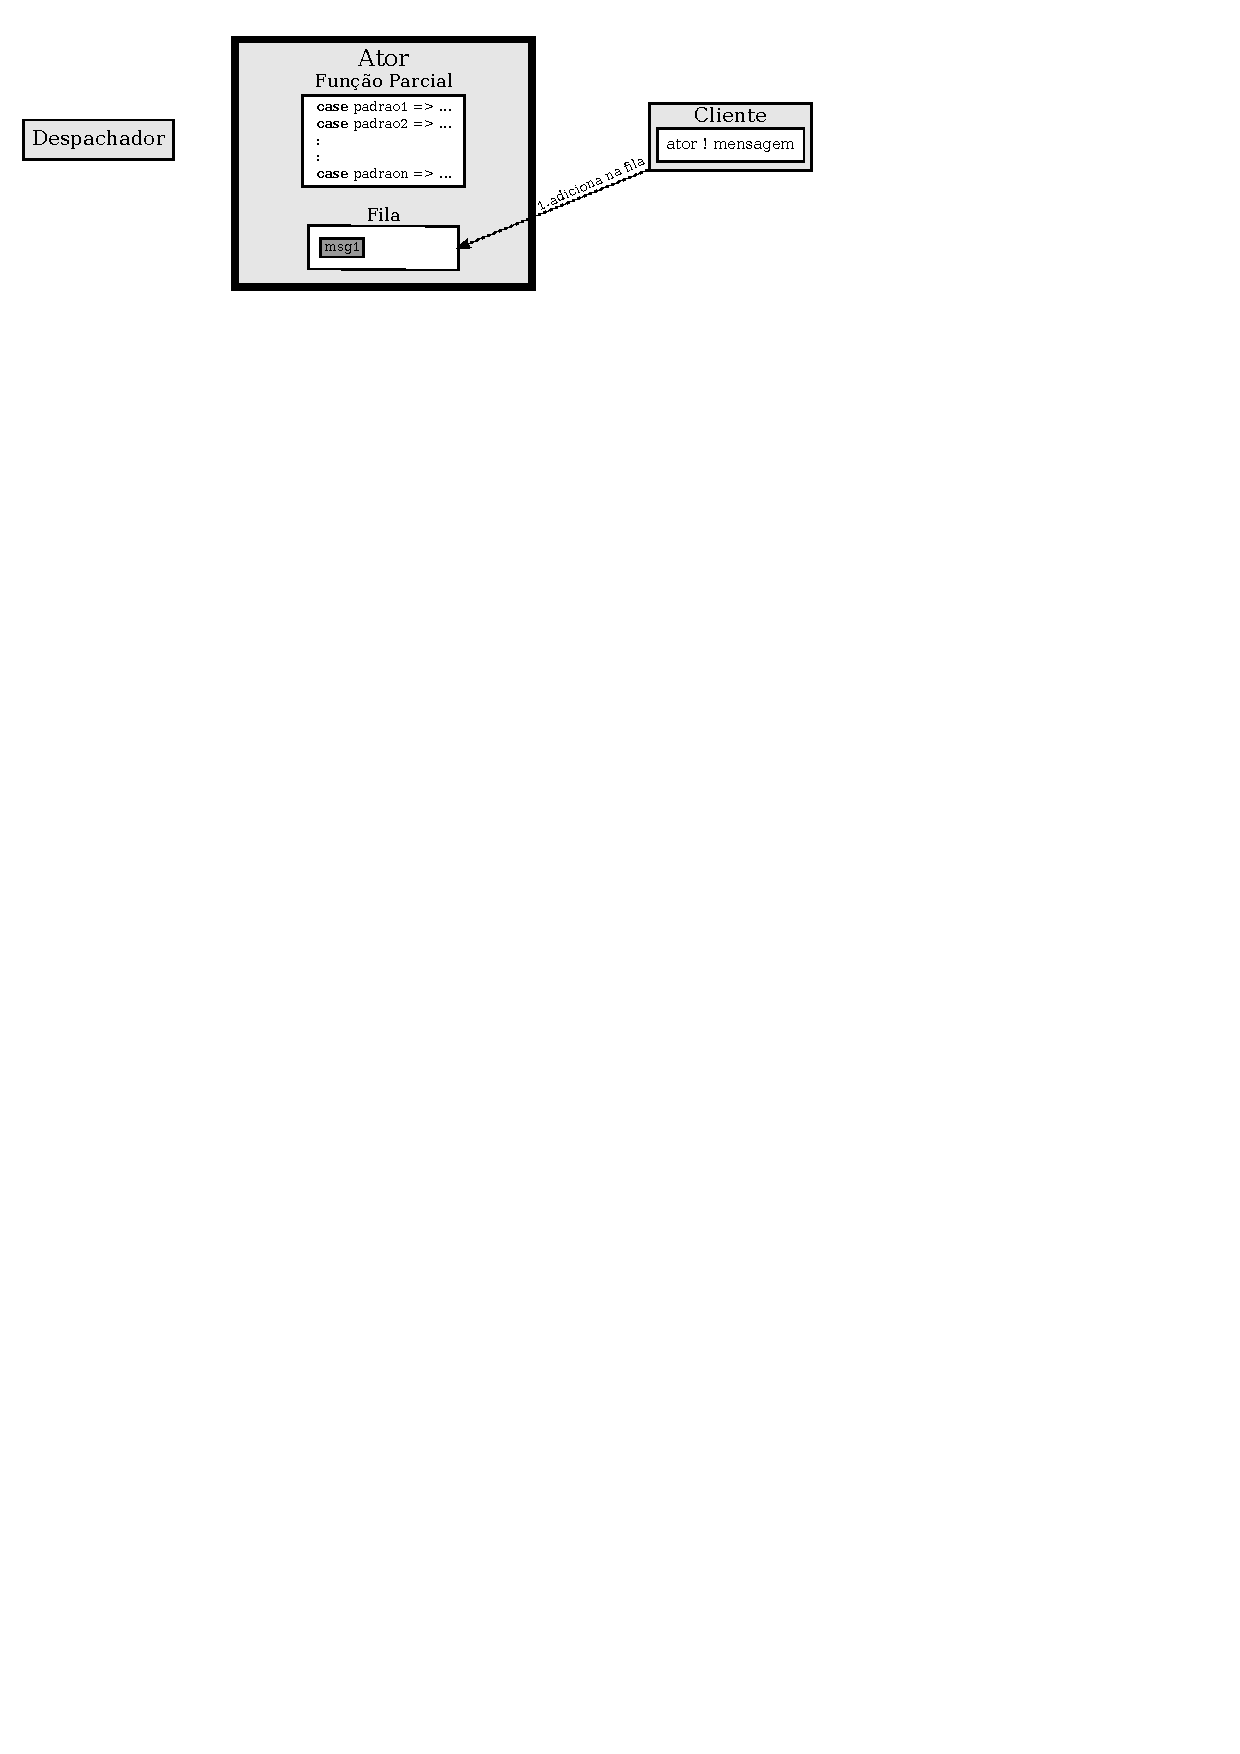
\includegraphics[scale=.70]{figuras/local-actor-message1.pdf}
		\end{figure}
 	}
	\only<3>{ 		
  		\begin{figure}[hbtp]
			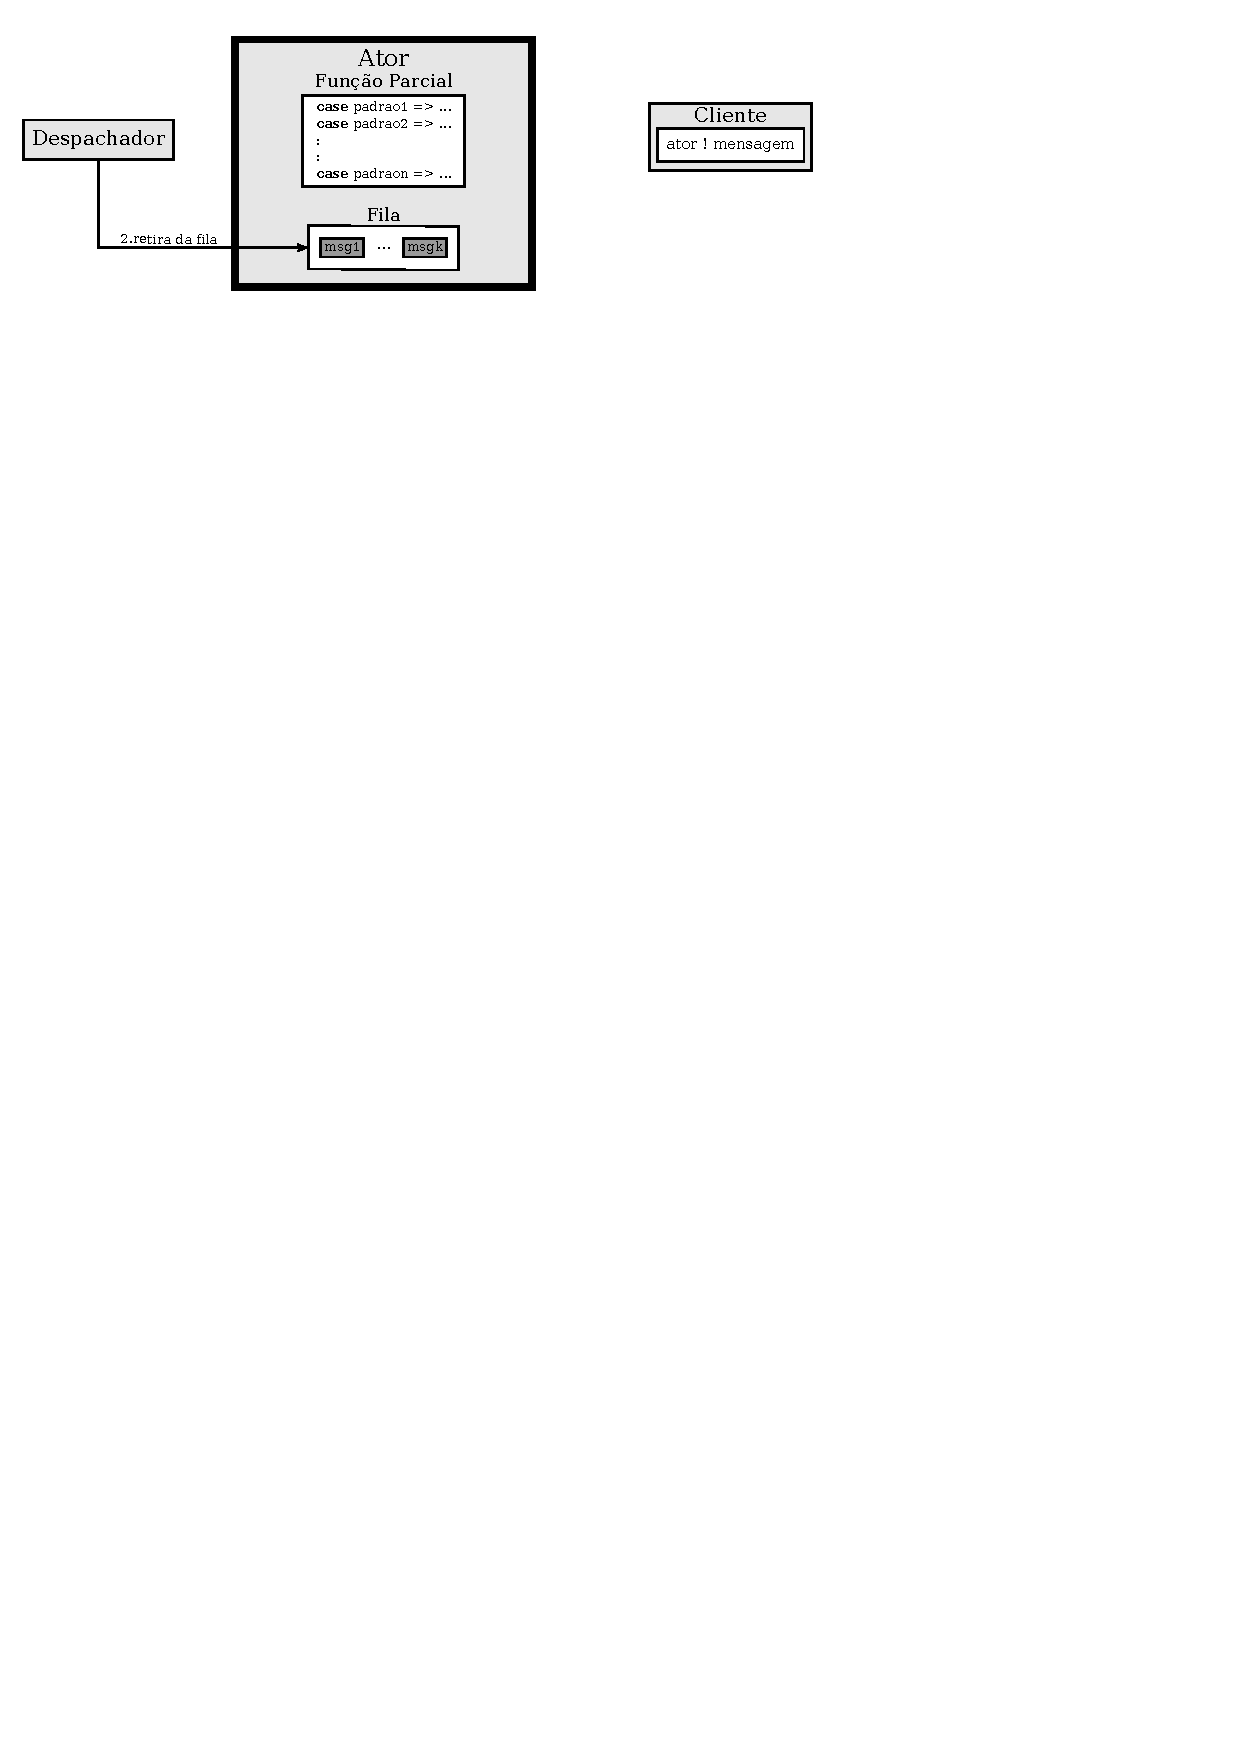
\includegraphics[scale=.70]{figuras/local-actor-message2.pdf}
		\end{figure}
 	}
	\only<4>{ 		
  		\begin{figure}[hbtp]
			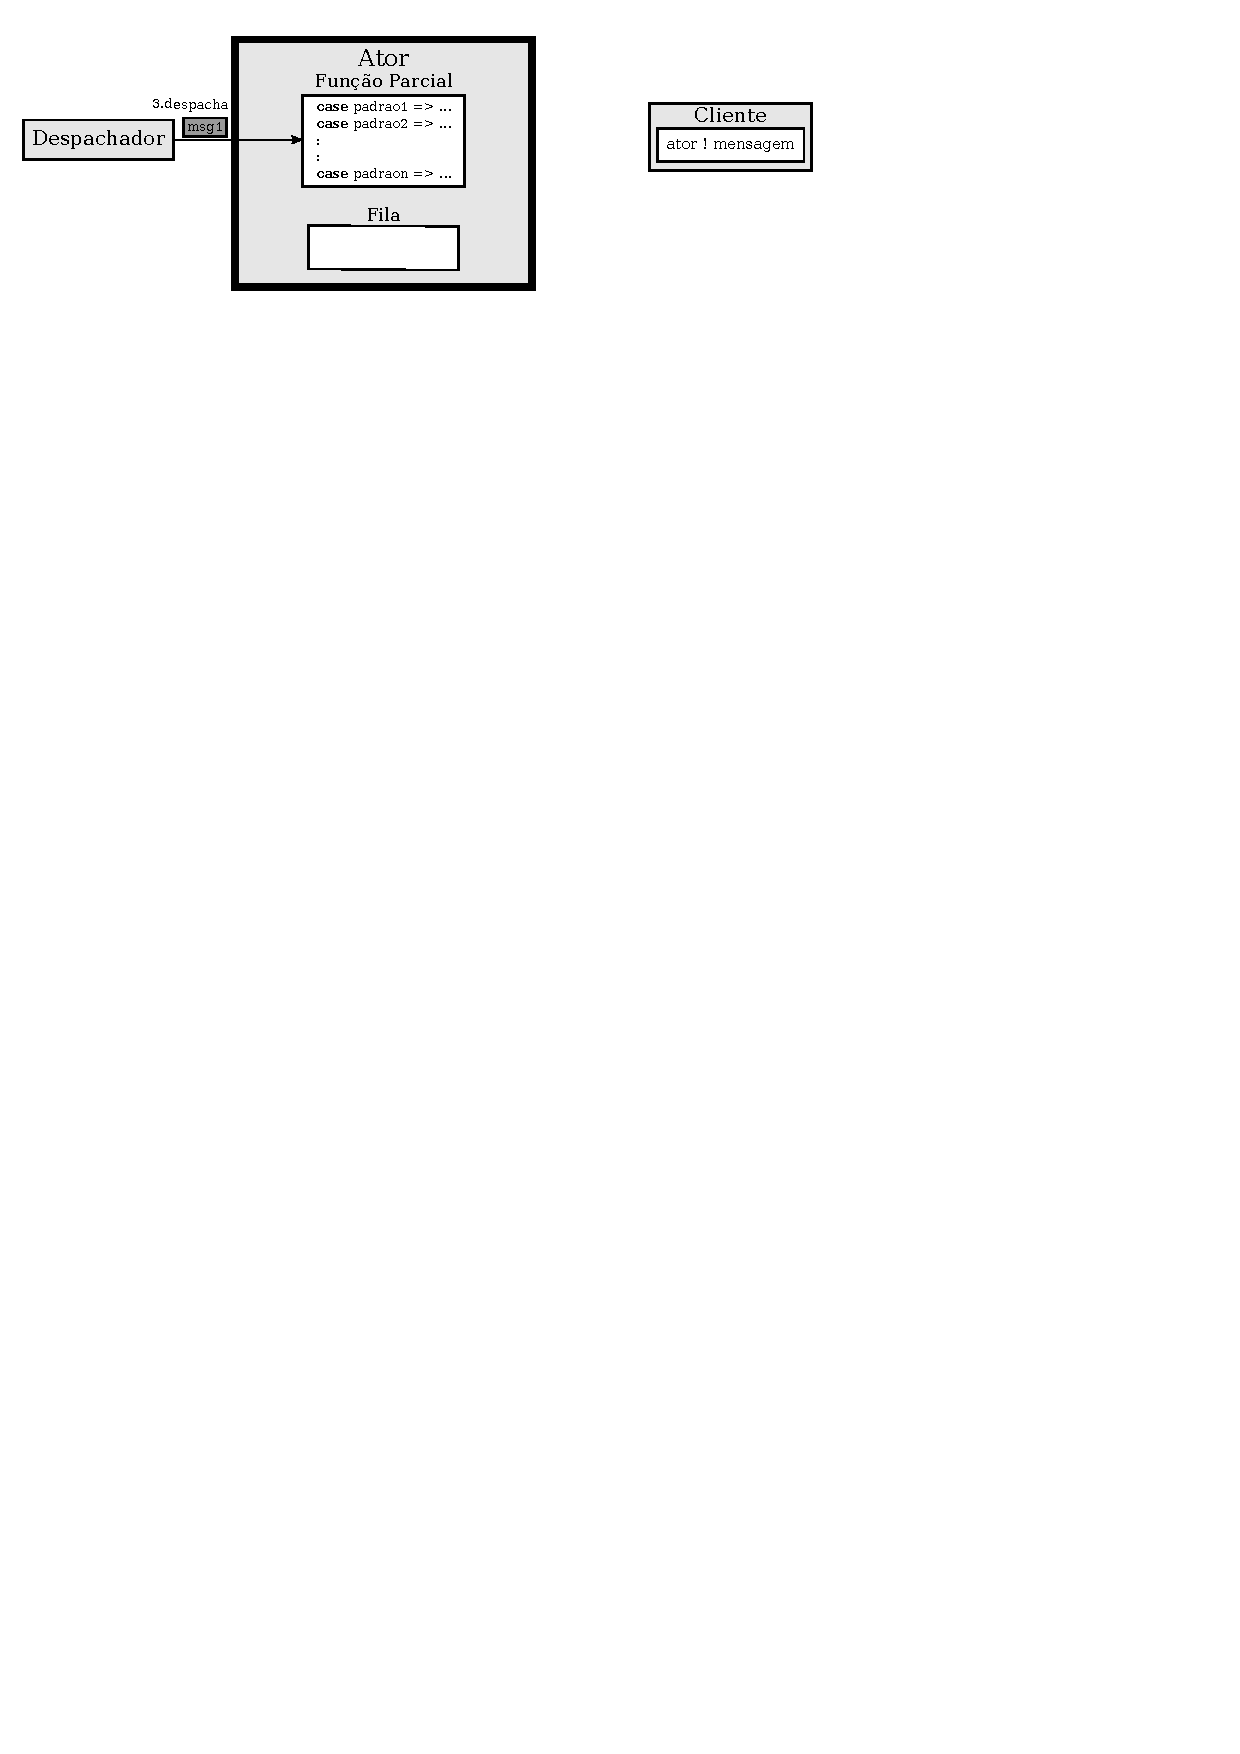
\includegraphics[scale=.70]{figuras/local-actor-message3.pdf}
		\end{figure}
 	}
}

\begin{frame}[fragile]{Envios s\'incronos com resposta -- !! e !!!}
\note{a diferenca para da interface do metodo !! para o metodo !!! eh o tipo de retorno. !!! devolve um Future[T].}
Interface do m\'etodo !!:
\begin{lstlisting}[frame=tb]
def !!(message: Any, timeout: Long = this.timeout) (implicit sender: Option[ActorRef] = None): Option[Any] = {
	...
}
\end{lstlisting}

Fei\c{c}\~ao CompletableFuture:
\begin{lstlisting}[frame=tb]
trait CompletableFuture[T] extends Future[T] {
  def completeWithResult(result: T)
  def completeWithException(exception: Throwable)
  def completeWith(other: Future[T])
}
\end{lstlisting}
\end{frame}
\frame{\frametitle{Envios s\'incronos com resposta -- !! e !!!}
	Passos executados na execu\c{c}\~ao do m\'etodo !!!:
 		\begin{enumerate}
			\item Uma inst\^ancia de CompletableFuture \'e criada
			\item A mensagem \'e depositada na fila do ator junto com uma refer\^encia para a inst\^ancia do passo $1$
			\item Uma outra refer\^encia para a inst\^ancia do passo $1$ \'e devolvida a quem fez a chamada do m\'etodo
			\item O resultado do processamento da mensagem \'e utilizado para completar a inst\^ancia criada no passo $1$
		\end{enumerate}
}

\subsection{Atores remotos}
\frame{\frametitle{Atores remotos}
	\only<1>{ 		
  		\begin{figure}[hbtp]
			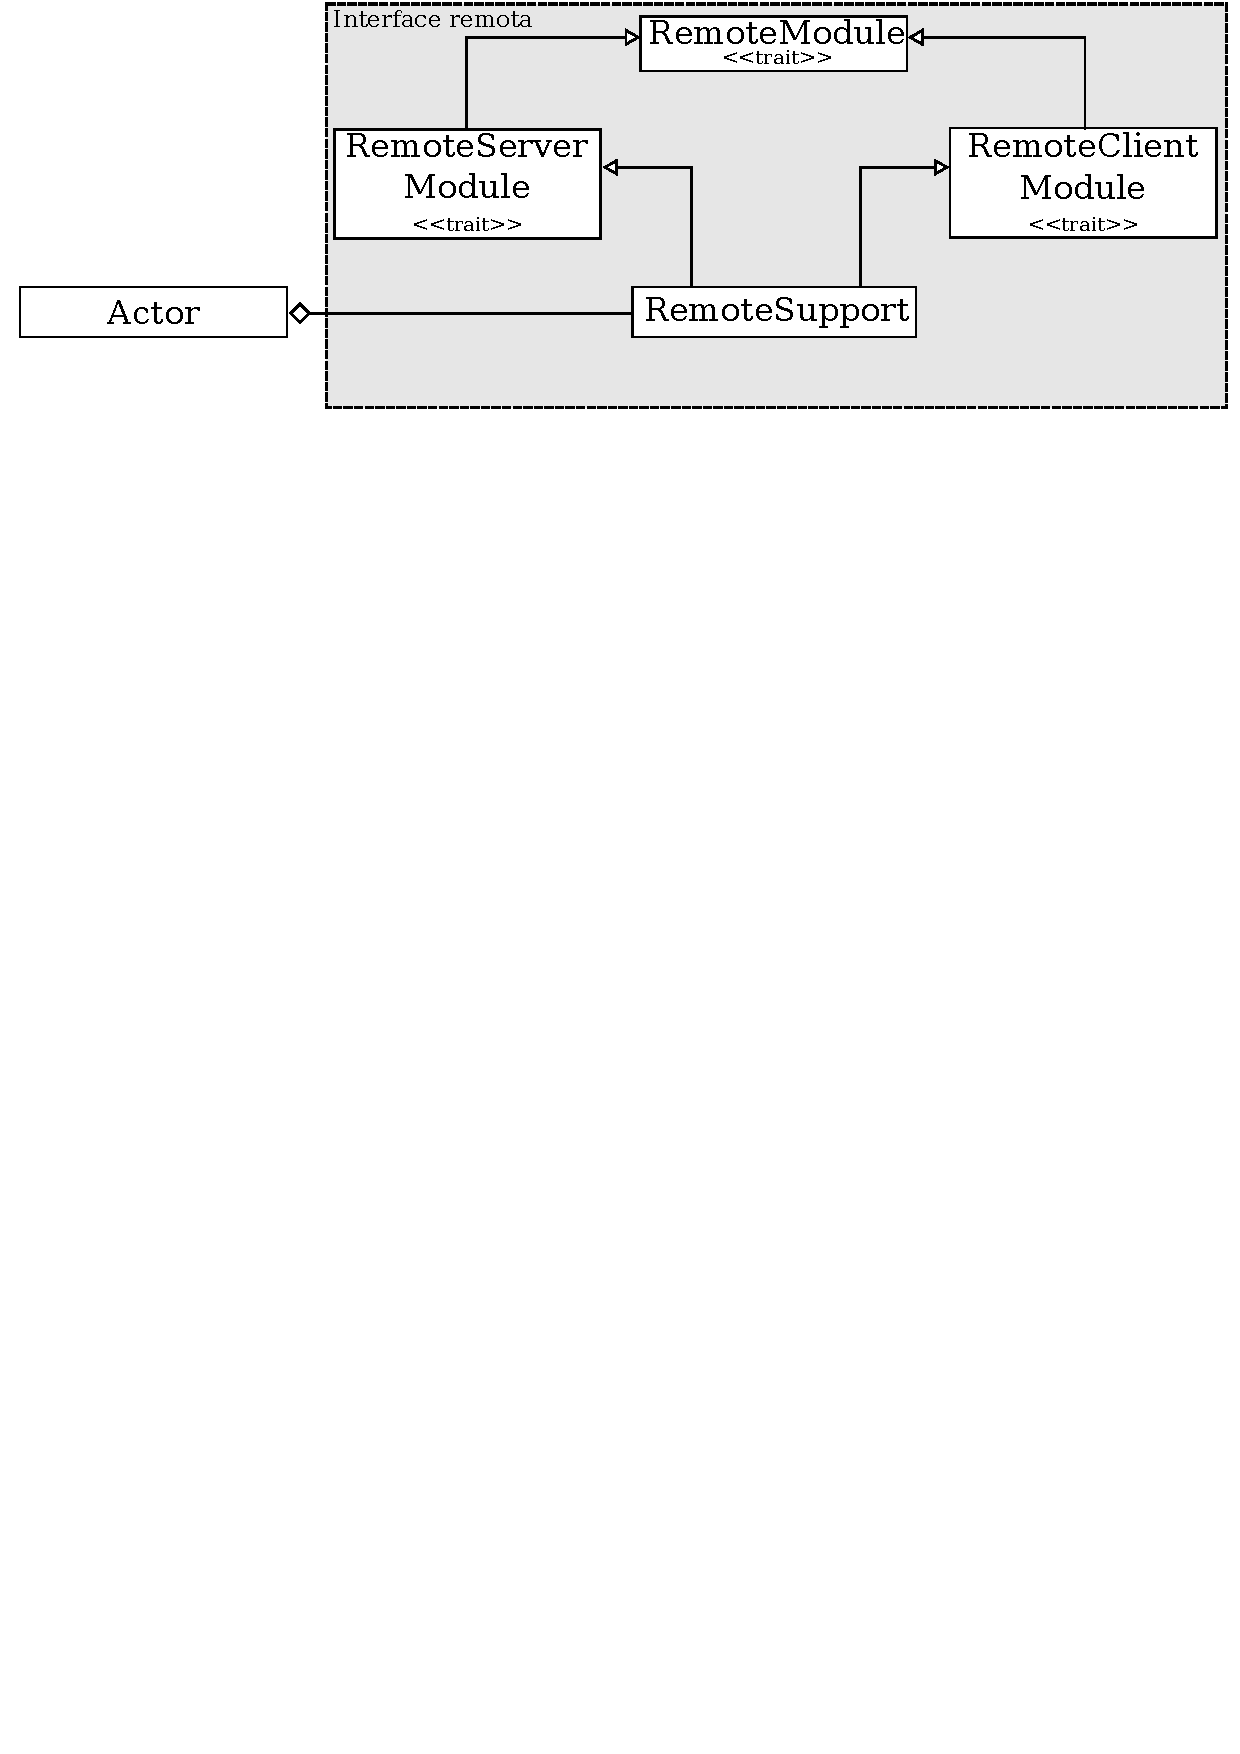
\includegraphics[scale=.50]{figuras/remote-actor-colaboracao0.pdf}
		\end{figure}
 	}
	\only<2>{ 		
  		\begin{figure}[hbtp]
			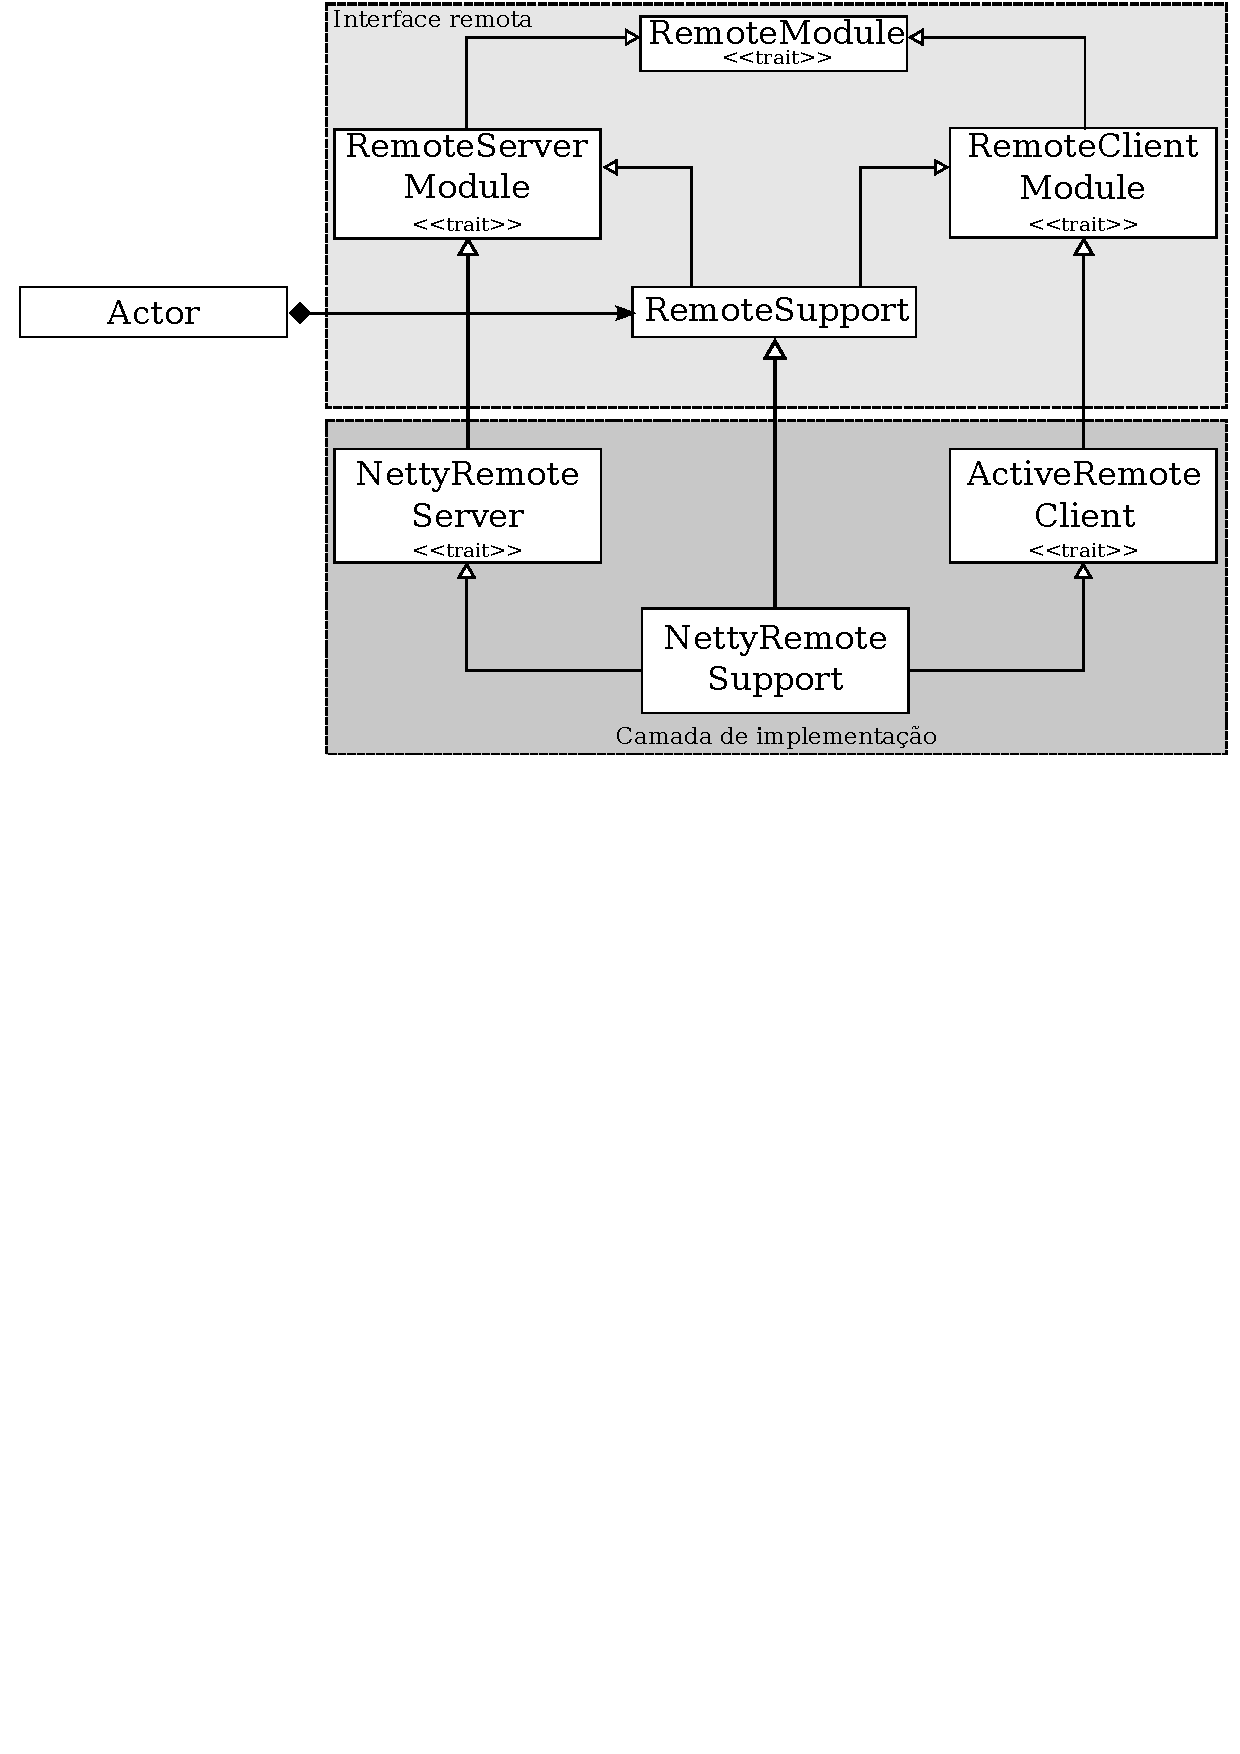
\includegraphics[scale=.50]{figuras/remote-actor-colaboracao.pdf}
		\end{figure}
 	}
}
\begin{frame}[fragile]{Atores remotos}

Registro de um ator remotamente acess\'ivel:
\begin{lstlisting}[frame=tb]
object SampleRemoteServer extends Application {
  Actor.remote.start("localhost", 2552)
  Actor.remote.register("hello-service", Actor.actorOf[SampleActor])
}
\end{lstlisting}

Pesquisa e uso de um ator remotamente aces\'ivel:

\begin{lstlisting}[frame=tb]
object SampleRemoteClient extends Application{
  /* helloActor representa uma RemoteActorRef */
  val helloActor = Actor.remote.actorFor("hello-service", "localhost", 2552)
  helloActor ! "Hello"
}
\end{lstlisting}
\end{frame}

\frame{\frametitle{Atores remotos}
	\only<1>{ 		
  		\begin{figure}[hbtp]
			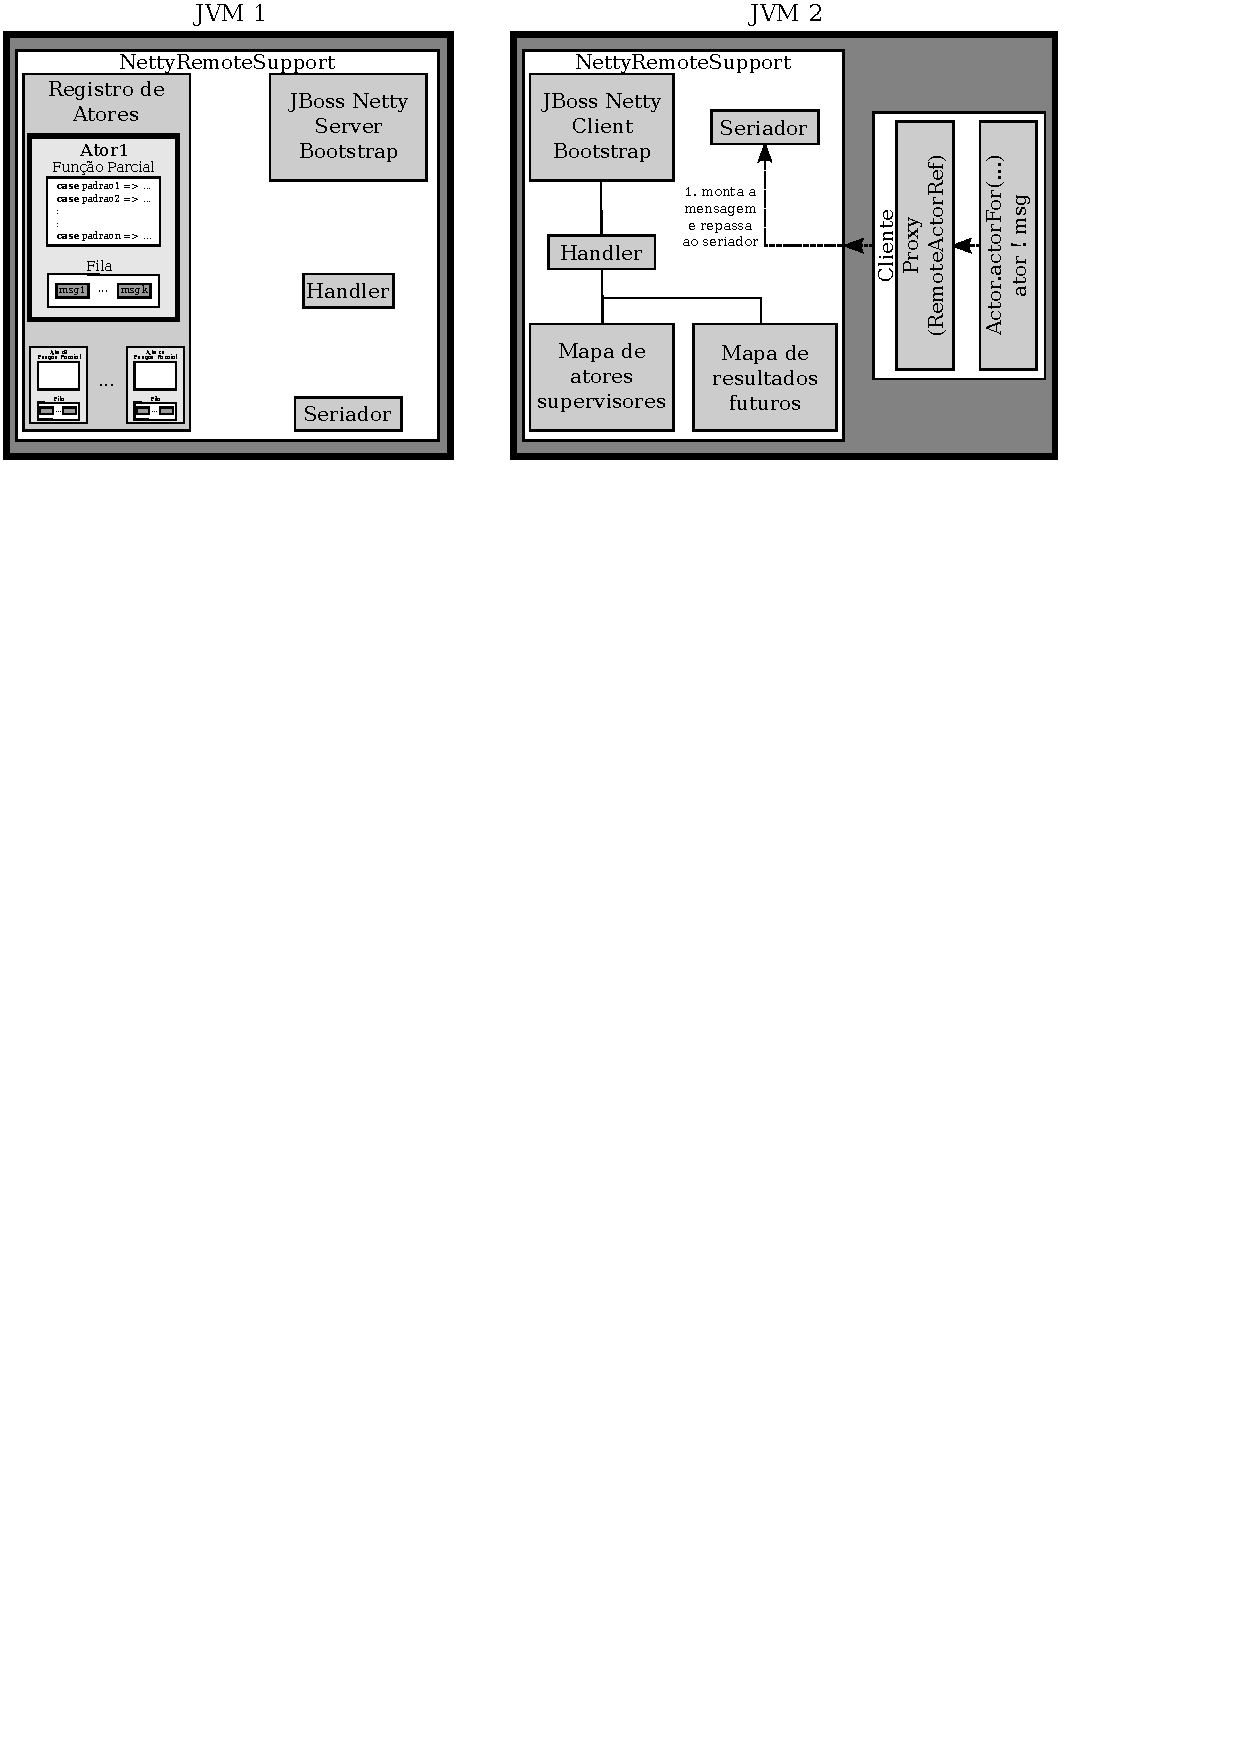
\includegraphics[scale=.50]{figuras/remote-actor-message-flow0.pdf}
		\end{figure}
 	}
	\only<2>{ 		
  		\begin{figure}[hbtp]
			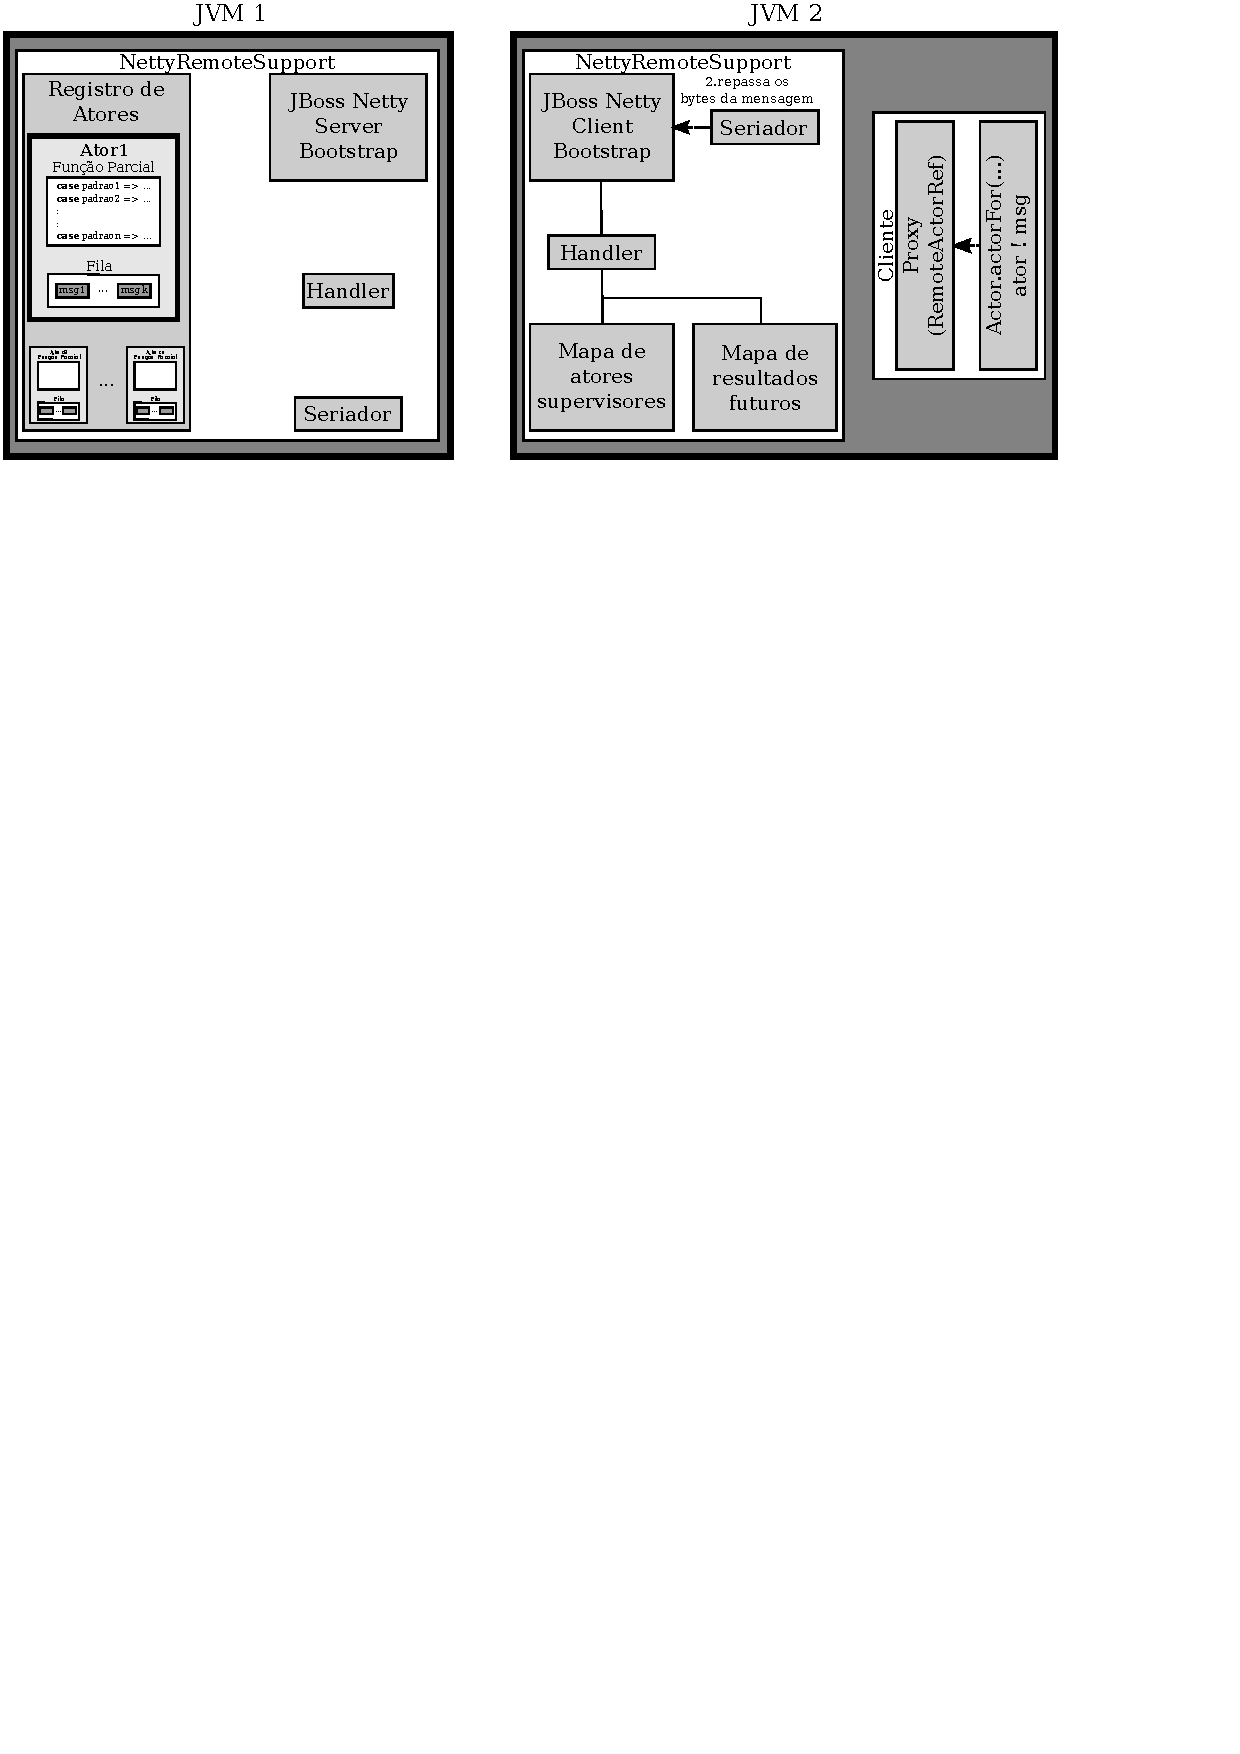
\includegraphics[scale=.50]{figuras/remote-actor-message-flow1.pdf}
		\end{figure}
 	}
	\only<3>{ 		
  		\begin{figure}[hbtp]
			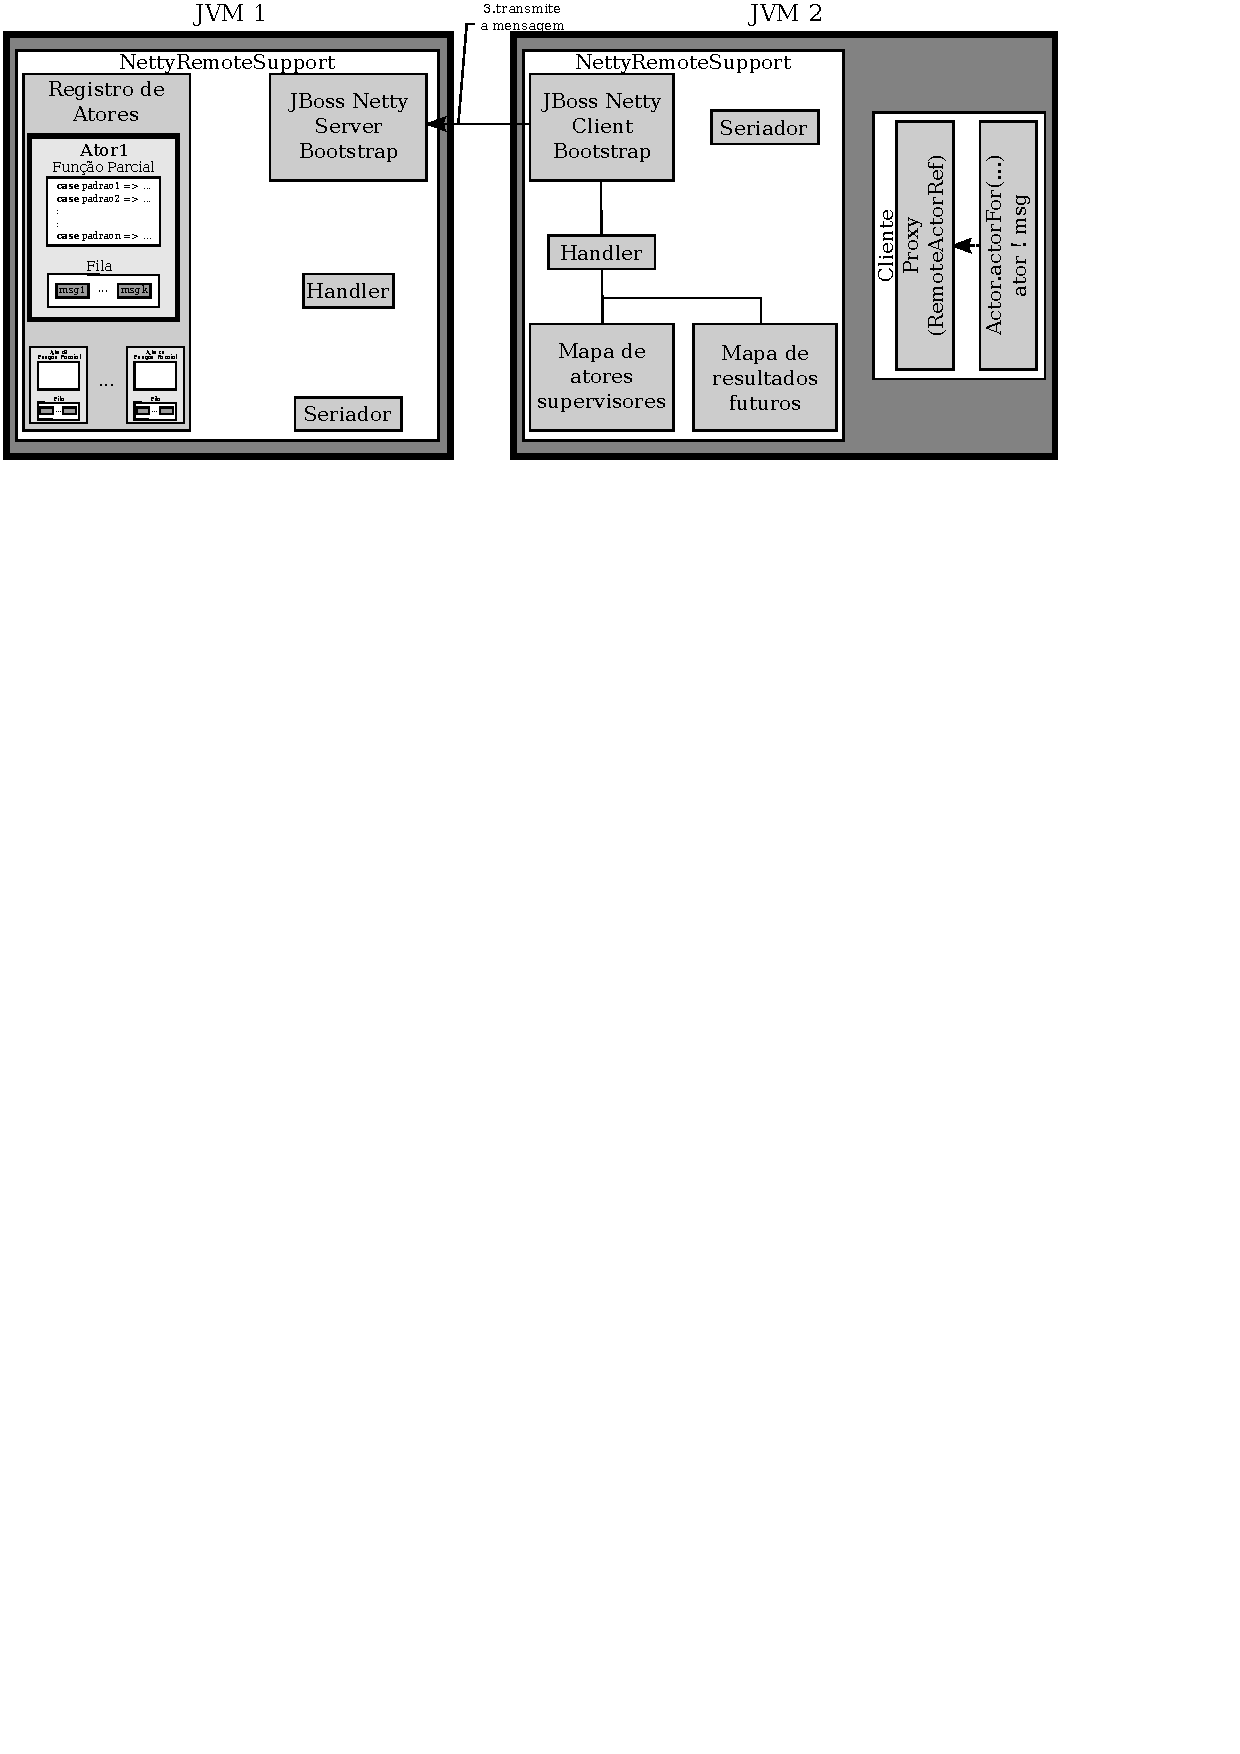
\includegraphics[scale=.50]{figuras/remote-actor-message-flow2.pdf}
		\end{figure}
 	}
	\only<4>{ 		
  		\begin{figure}[hbtp]
			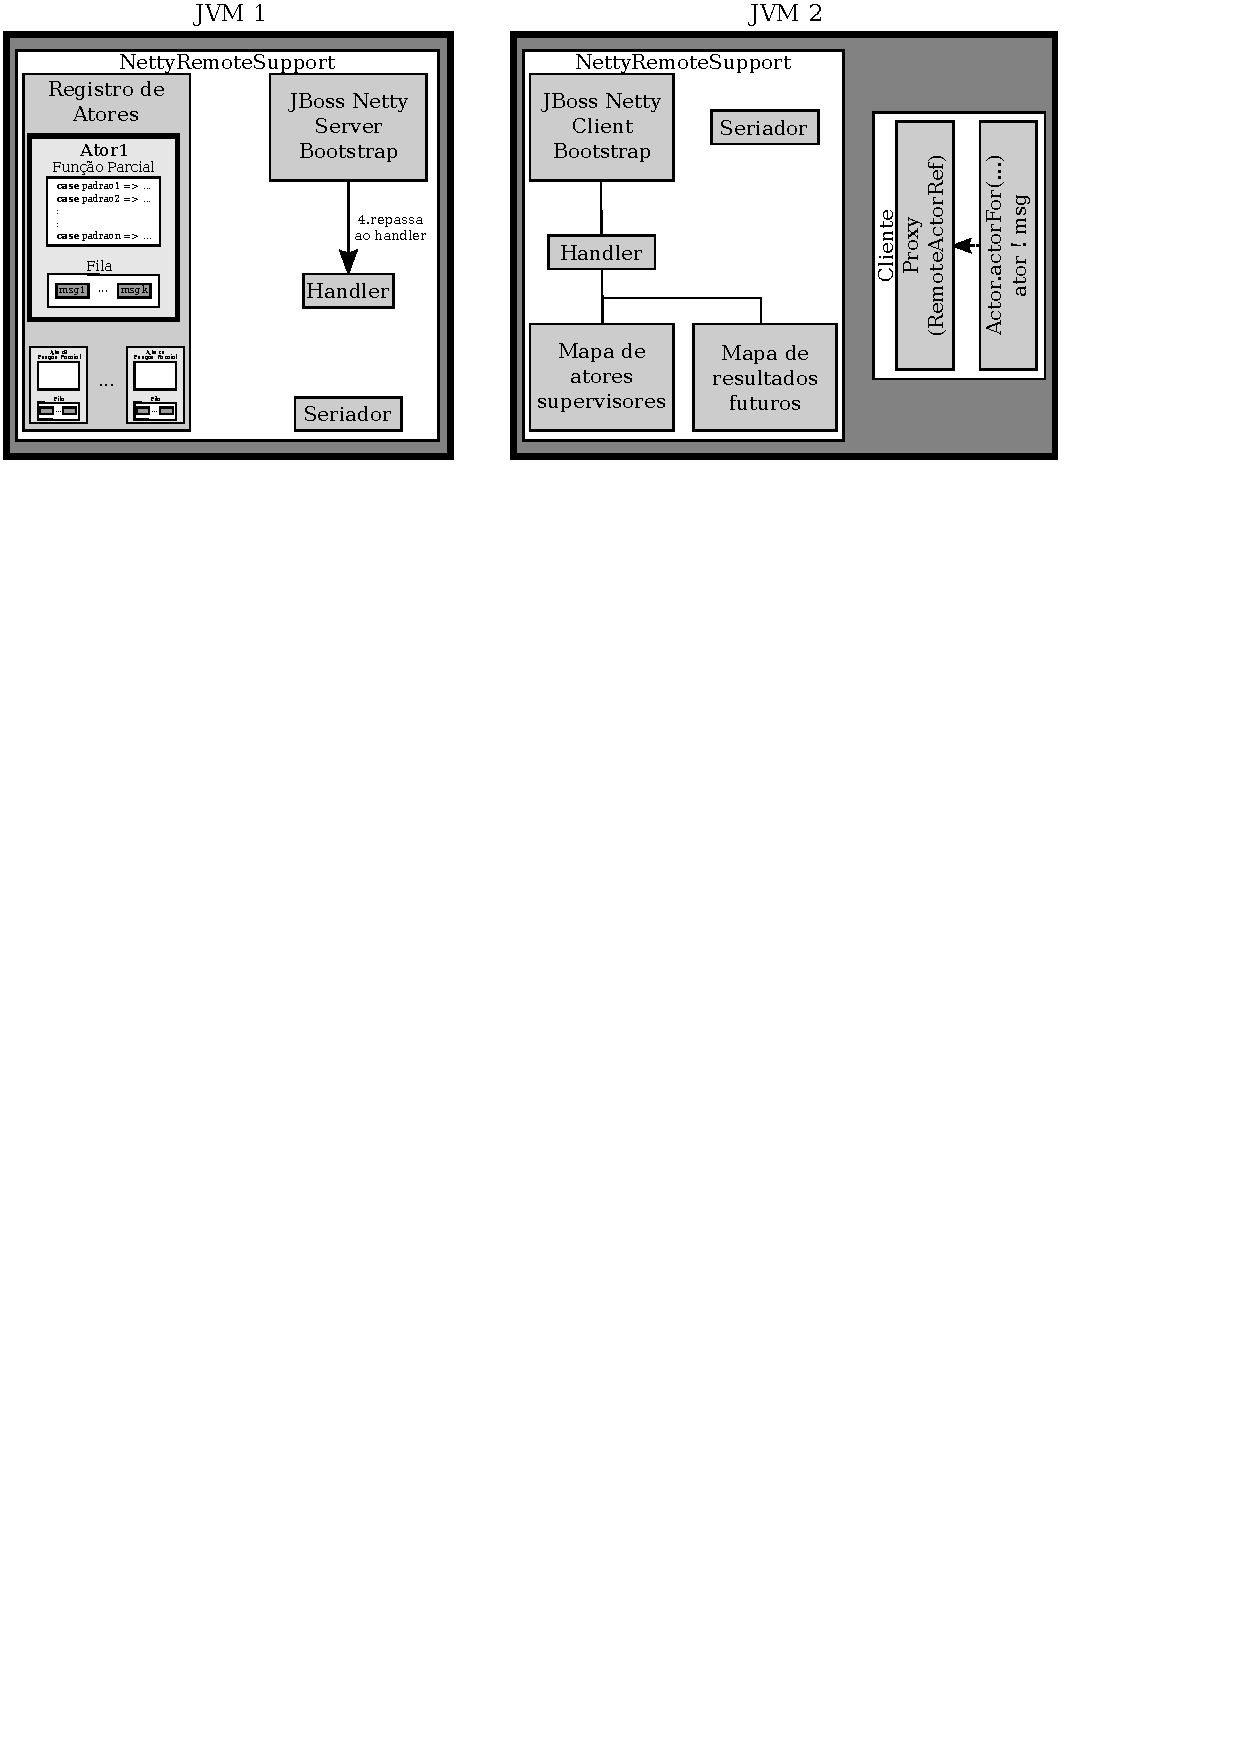
\includegraphics[scale=.50]{figuras/remote-actor-message-flow3.pdf}
		\end{figure}
 	}
	\only<5>{ 		
  		\begin{figure}[hbtp]
			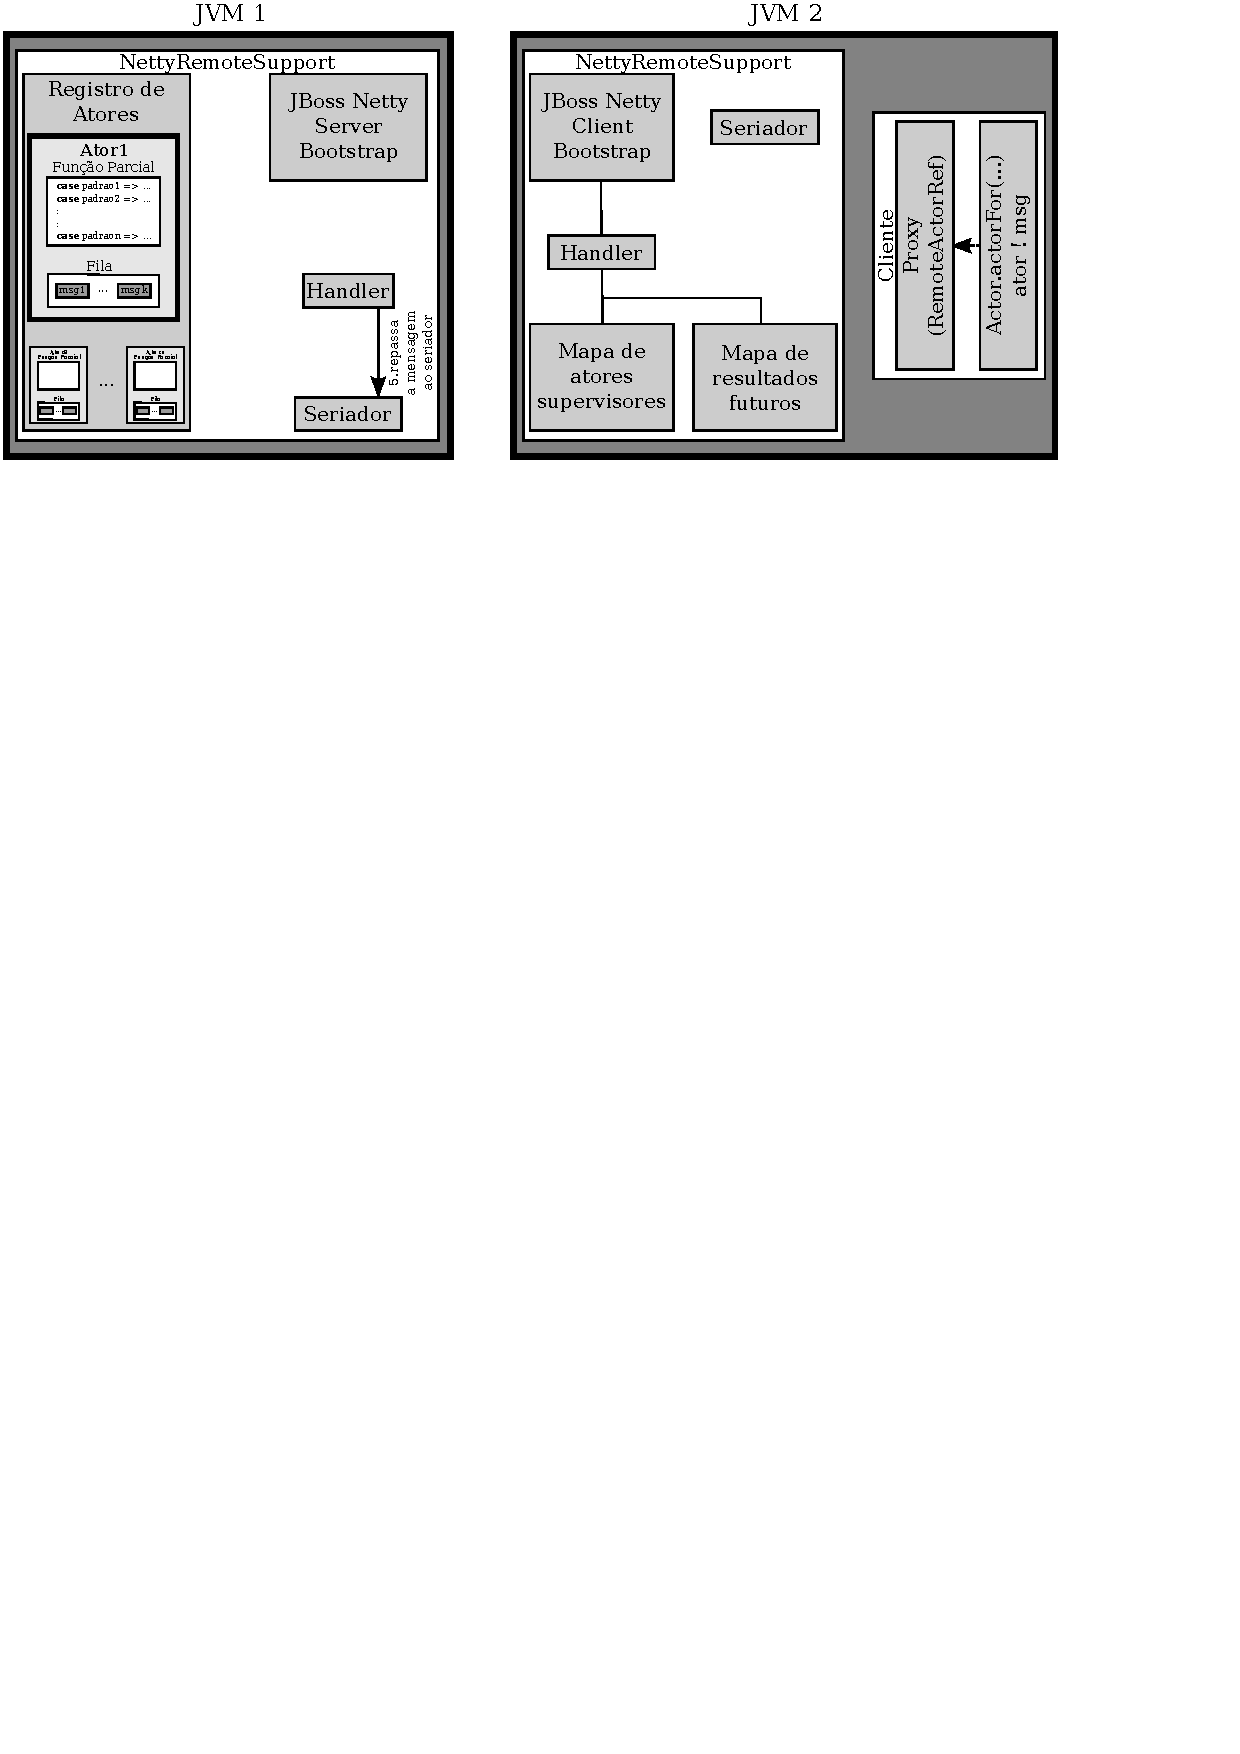
\includegraphics[scale=.50]{figuras/remote-actor-message-flow4.pdf}
		\end{figure}
 	}
	\only<6>{ 		
  		\begin{figure}[hbtp]
			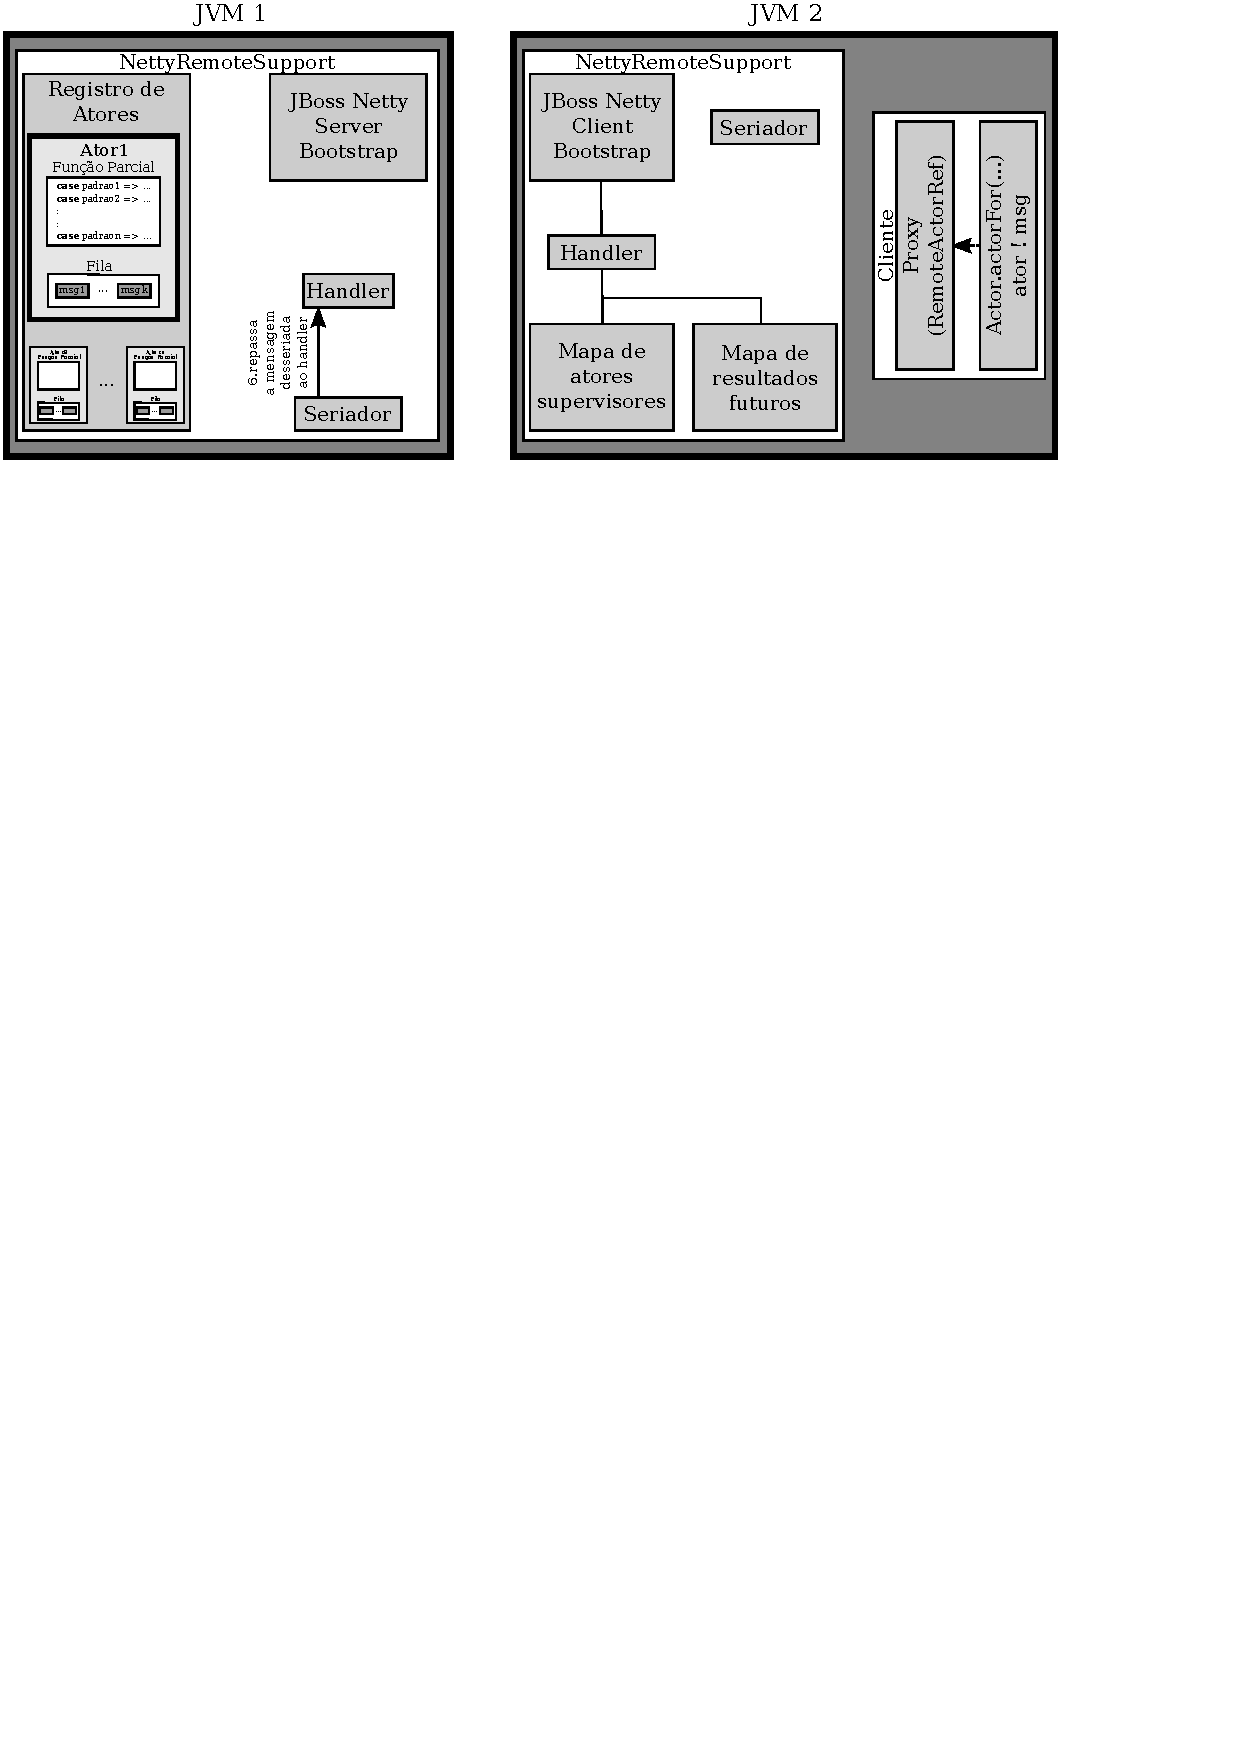
\includegraphics[scale=.50]{figuras/remote-actor-message-flow5.pdf}
		\end{figure}
 	}
	\only<7>{ 		
  		\begin{figure}[hbtp]
			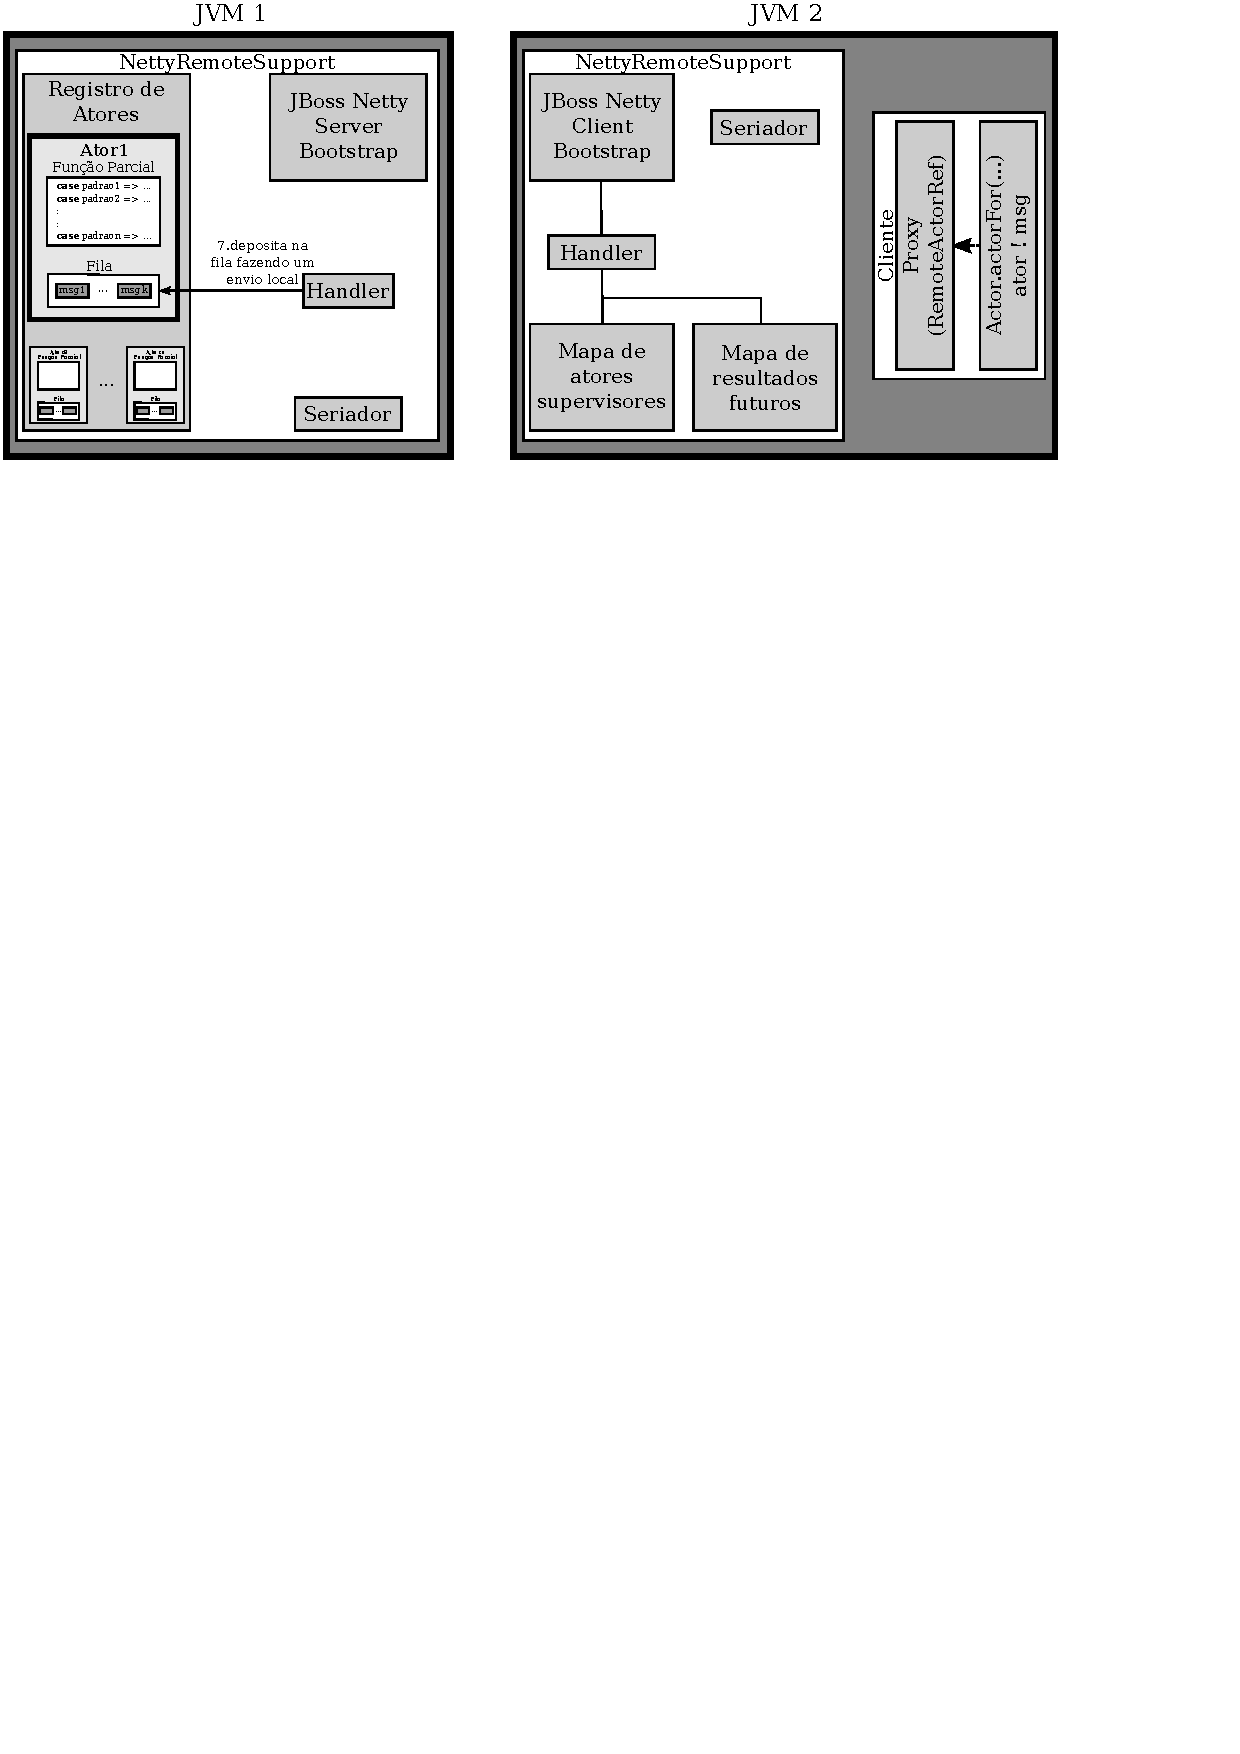
\includegraphics[scale=.50]{figuras/remote-actor-message-flow6.pdf}
		\end{figure}
 	}
}

\begin{frame}[fragile]{Formato e seria\c{c}\~ao das mensagens}
\begin{lstlisting}[frame=tb]
message RemoteMessageProtocol {
  required UuidProtocol uuid = 1;
  required ActorInfoProtocol actorInfo = 2;
  required bool oneWay = 3;
  optional MessageProtocol message = 4; // <- payload da mensagem
  optional ExceptionProtocol exception = 5;
  optional UuidProtocol supervisorUuid = 6;
  optional RemoteActorRefProtocol sender = 7;
  repeated MetadataEntryProtocol metadata = 8;
  optional string cookie = 9;
}
\end{lstlisting}

\begin{beamerboxesrounded}{Formatos suportados de seria\c{c}\~ao:}
 	\begin{itemize}
		\item Java, SBinary, JSON e Protobuf
	\end{itemize}		
\end{beamerboxesrounded}

\end{frame}

\section{Atores remotos com padr\~ao AMQP} 
\subsection{Pontes AMQP}
\frame{\frametitle{Estrutura das pontes AMQP}
	\only<1>{
 		Caracter\'isticas:
		\begin{itemize}
			\item As entidades passam a ser rotuladas por nome (e.g.: node1)
			\item Dois tipos de pontes AMQP para acesso ao \textit{message broker}:
				\begin{enumerate}
					\item ServerAMQPBridge: Define o comportamento para entidades com papel de servidora
					\item ClientAMQPBridge: Define o comportamento para entidades com papel de cliente				
				\end{enumerate}
			\item Suporte a acesso concorrente \`as pontes 
			\item Suporte a separa\c{c}\~ao do fluxo de leitura/escrita em canais distintos
			\item Suporte a cria\c{c}\~ao de objetos dur\'aveis, transientes ou exclusivos com auto remo\c{c}\~ao
		\end{itemize}
	}
	\only<2>{
 		\begin{figure}[hbtp]
			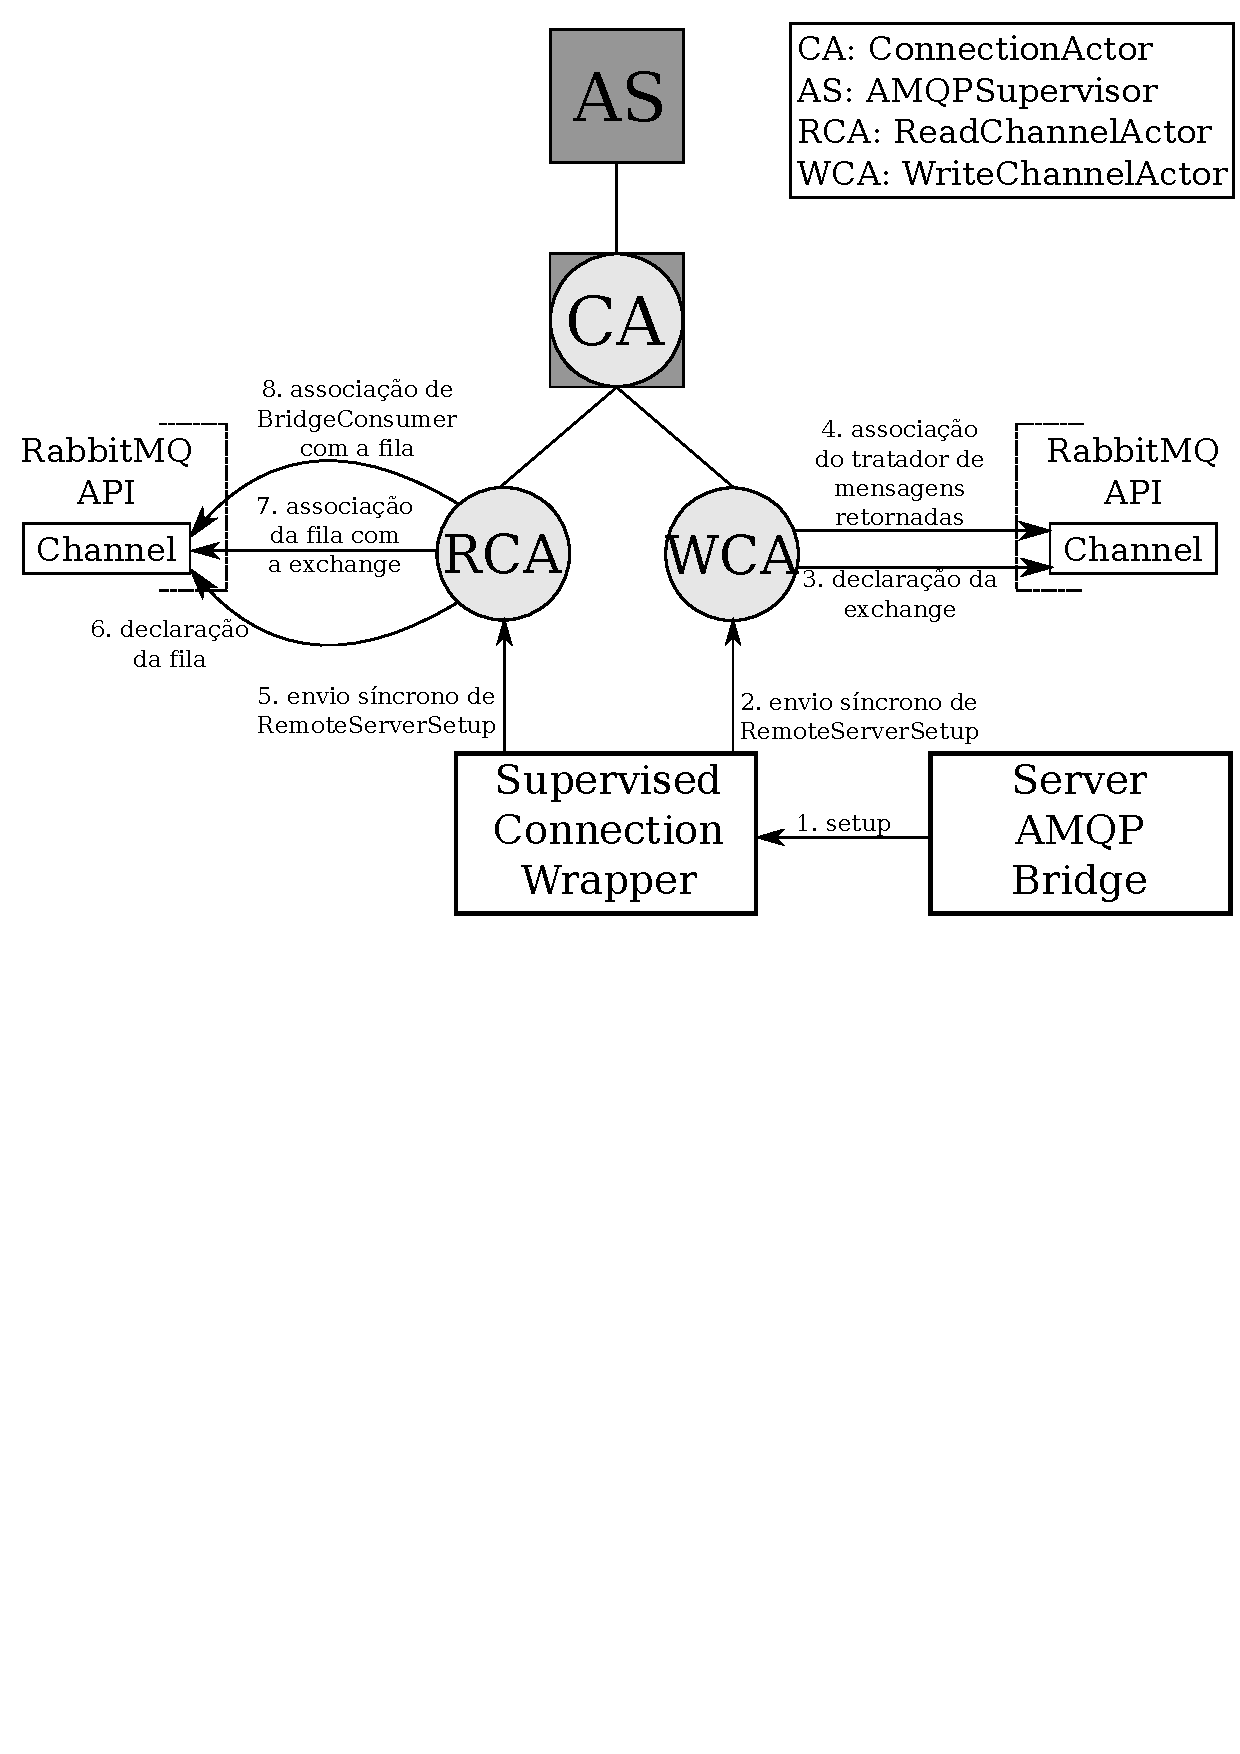
\includegraphics[scale=.35]{figuras/server-amqp-bridge-setup.pdf}
		\end{figure}
 	}
	\only<3>{
 		\begin{figure}[hbtp]
			
\includegraphics[scale=.50]{figuras/bridges-broker-all-together0.pdf}
		\end{figure}
 	}
	\only<4>{
 		\begin{figure}[hbtp]
			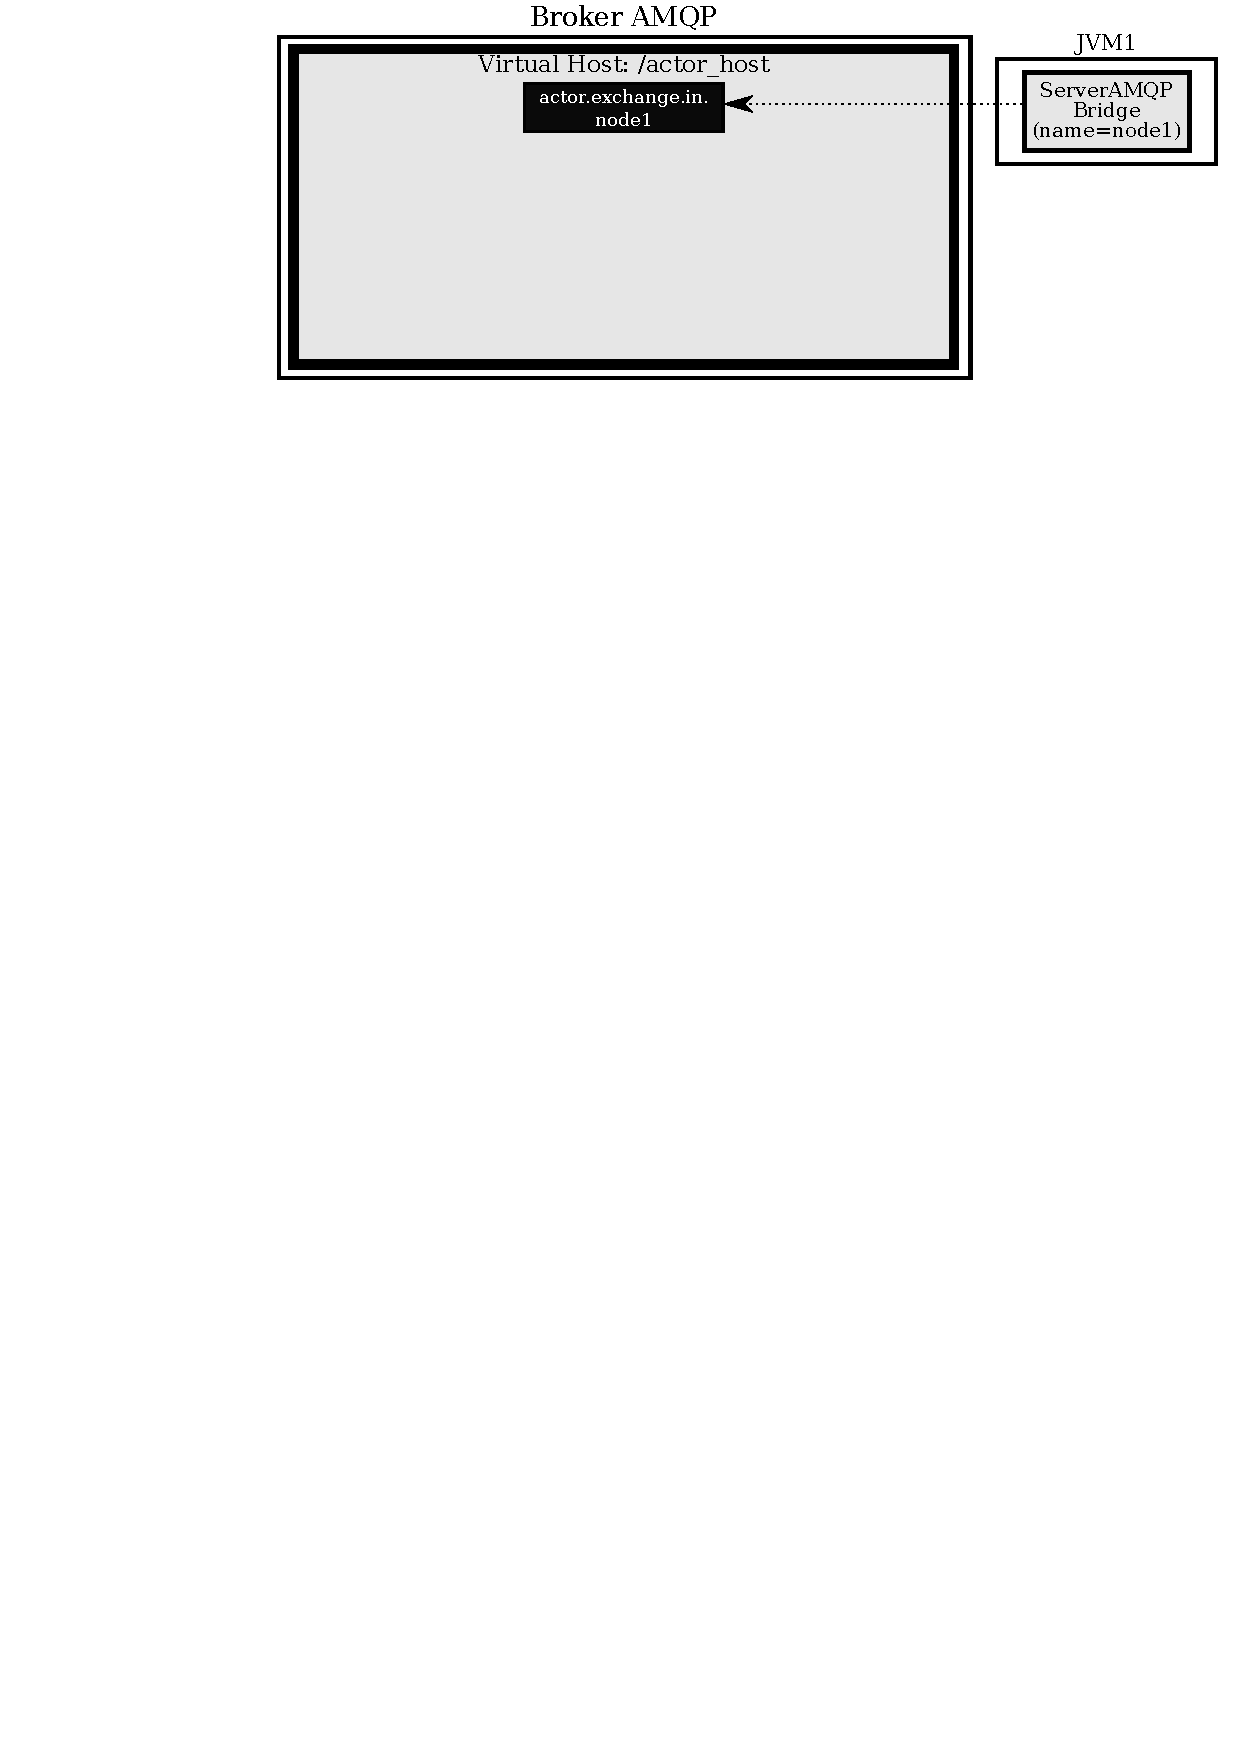
\includegraphics[scale=.50]{figuras/bridges-broker-all-together1.pdf}
		\end{figure}
 	}
	\only<5>{
 		\begin{figure}[hbtp]
			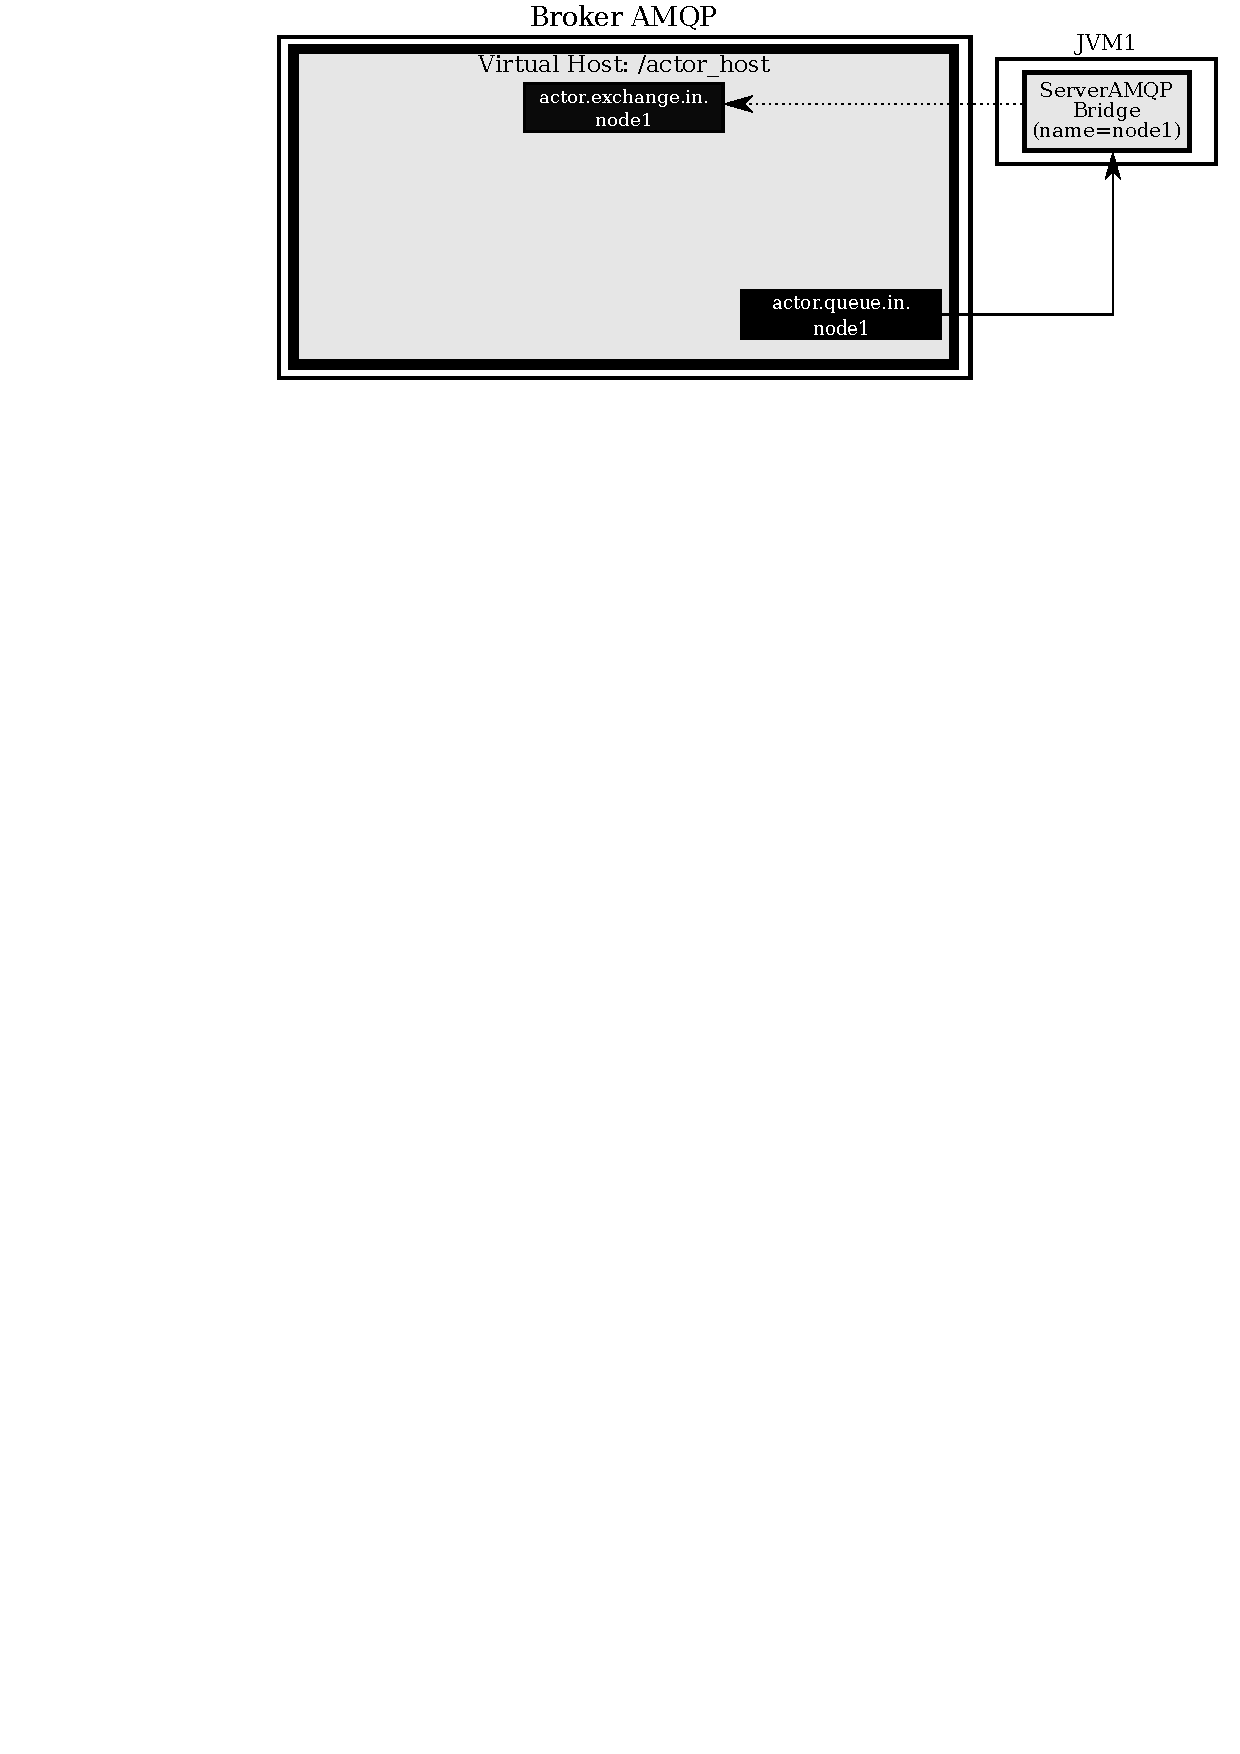
\includegraphics[scale=.50]{figuras/bridges-broker-all-together2.pdf}
		\end{figure}
 	}
	\only<6>{
 		\begin{figure}[hbtp]
			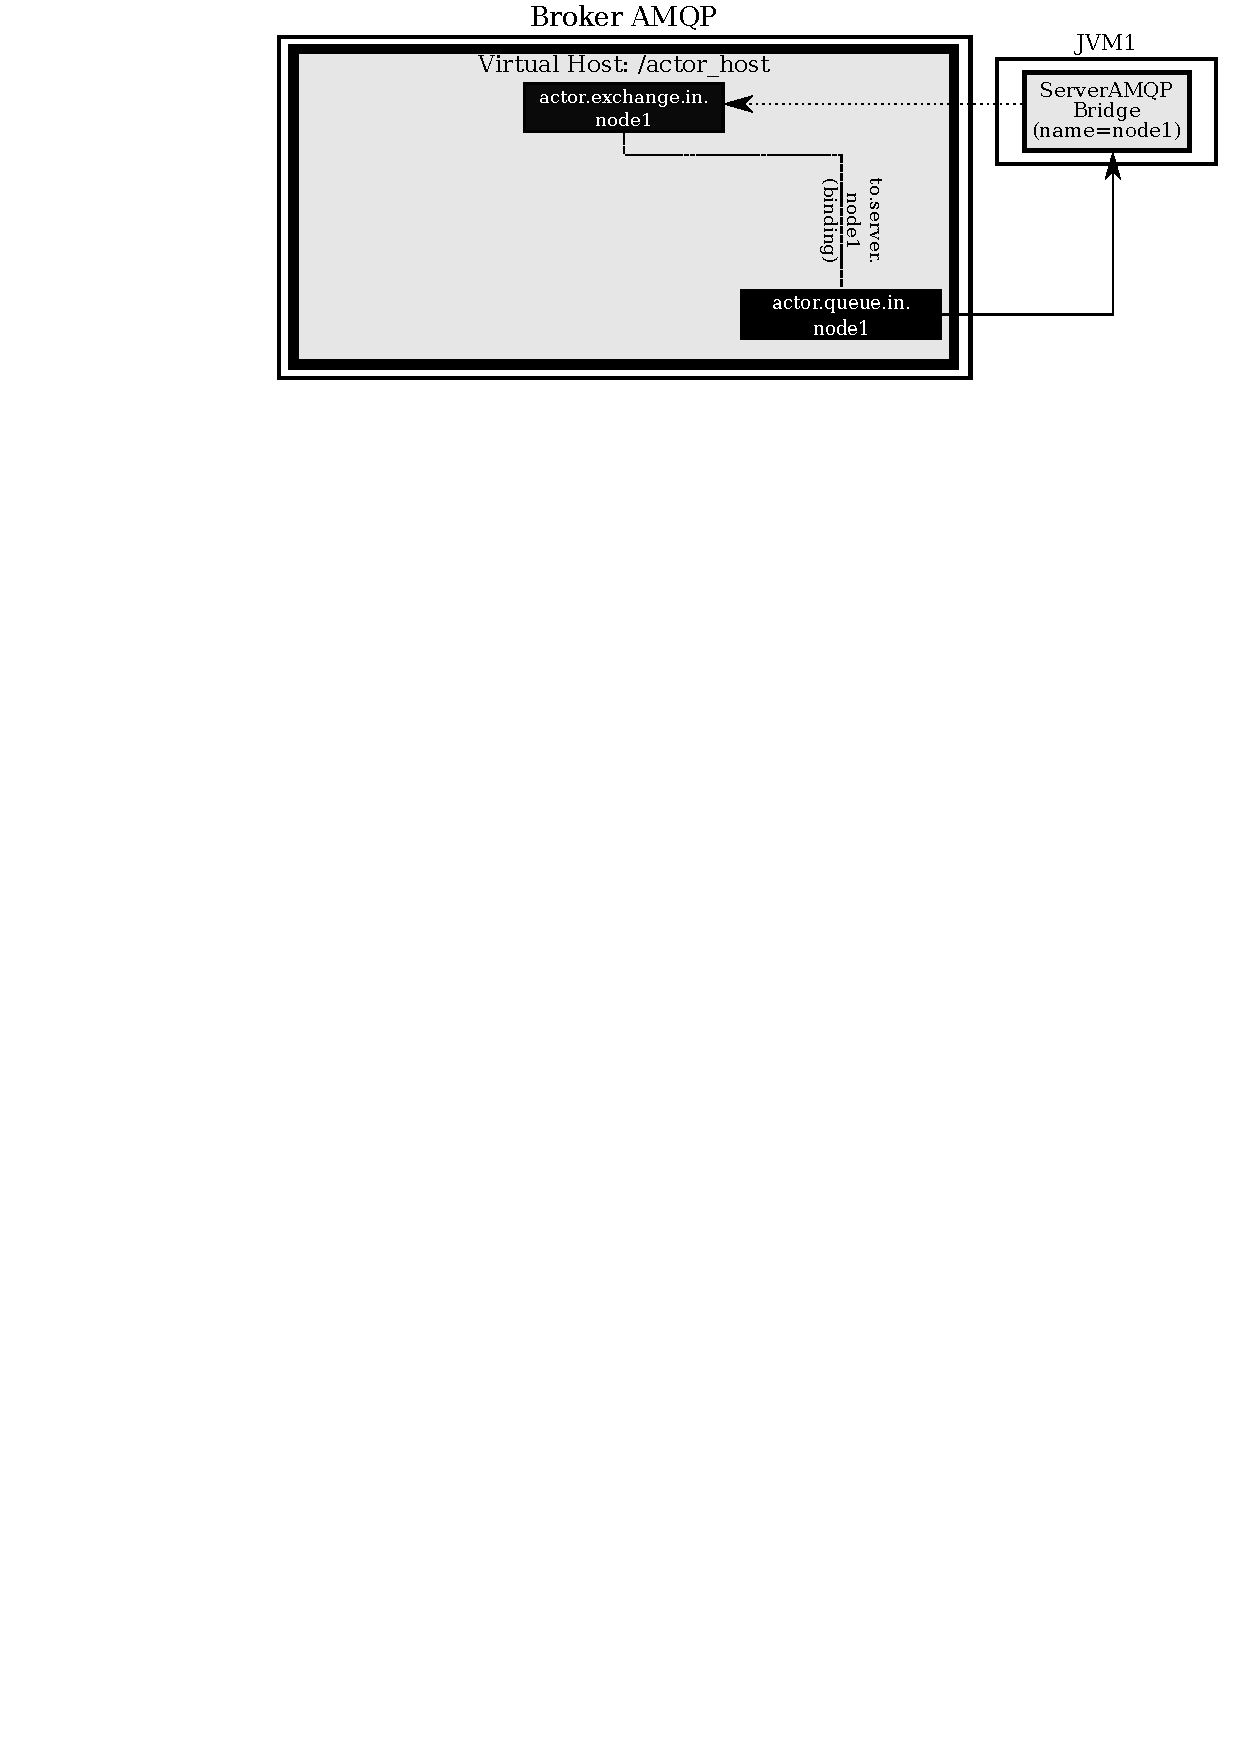
\includegraphics[scale=.50]{figuras/bridges-broker-all-together3.pdf}
		\end{figure}
 	}
	\only<7>{
 		\begin{figure}[hbtp]
			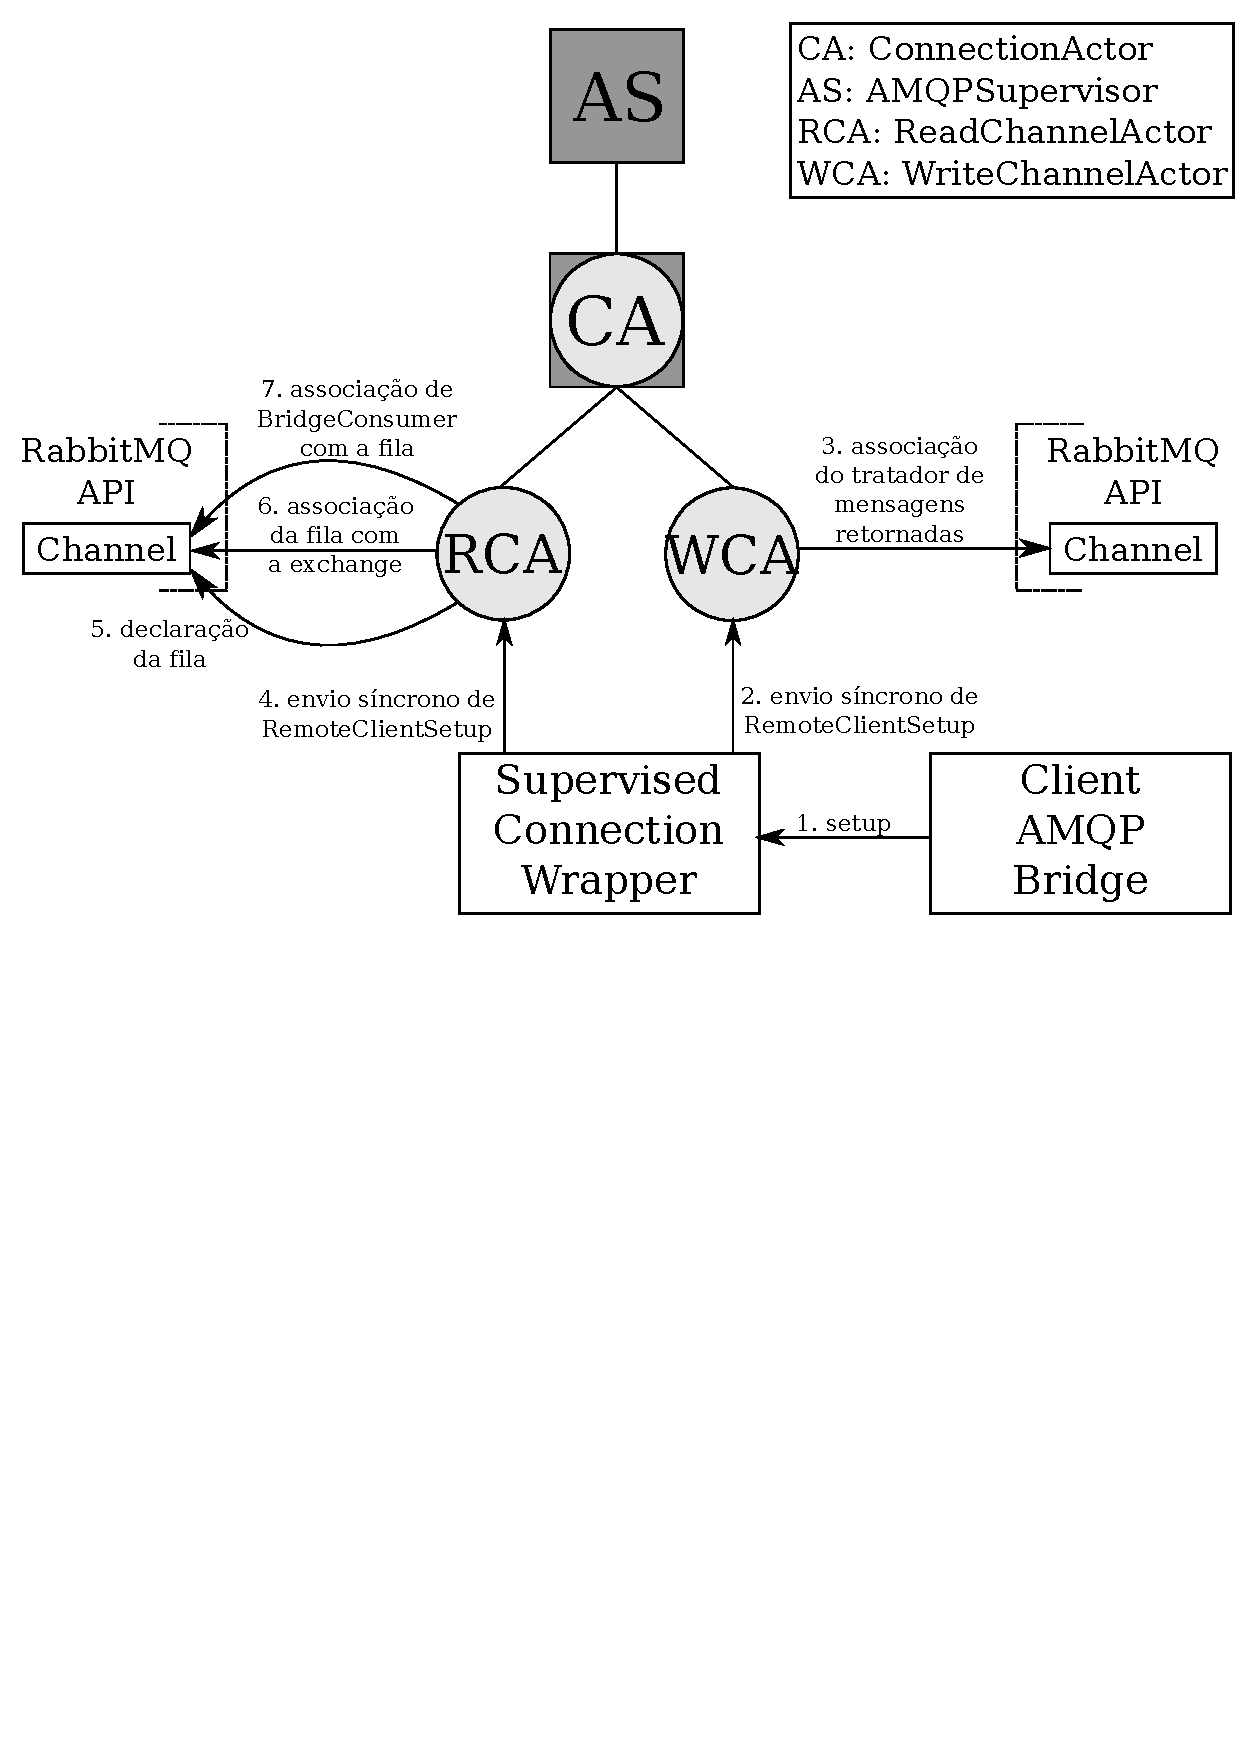
\includegraphics[scale=.35]{figuras/client-amqp-bridge-setup.pdf}
		\end{figure}
 	}
	\only<8>{
 		\begin{figure}[hbtp]
			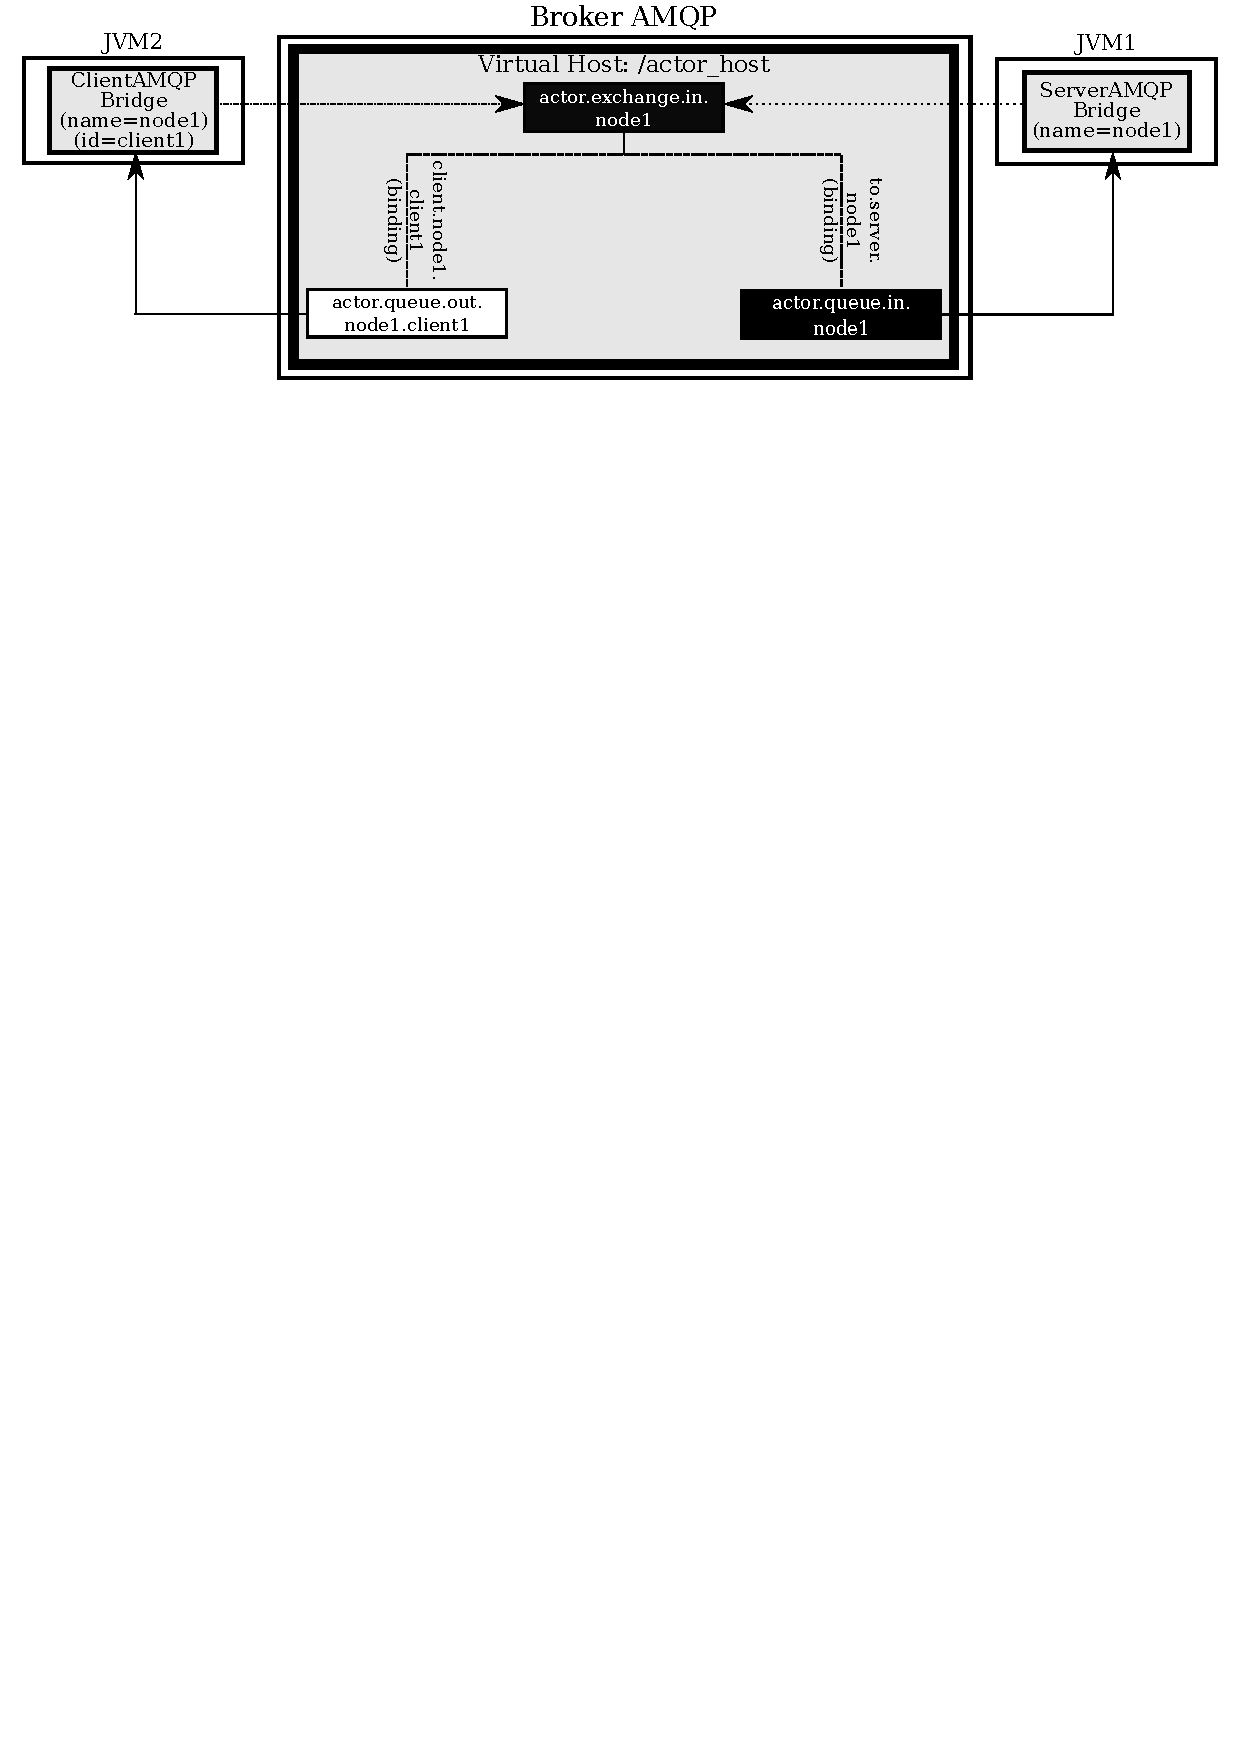
\includegraphics[scale=.50]{figuras/bridges-broker-all-together4.pdf}
		\end{figure}
 	}
	\only<9>{
 		\begin{figure}[hbtp]
			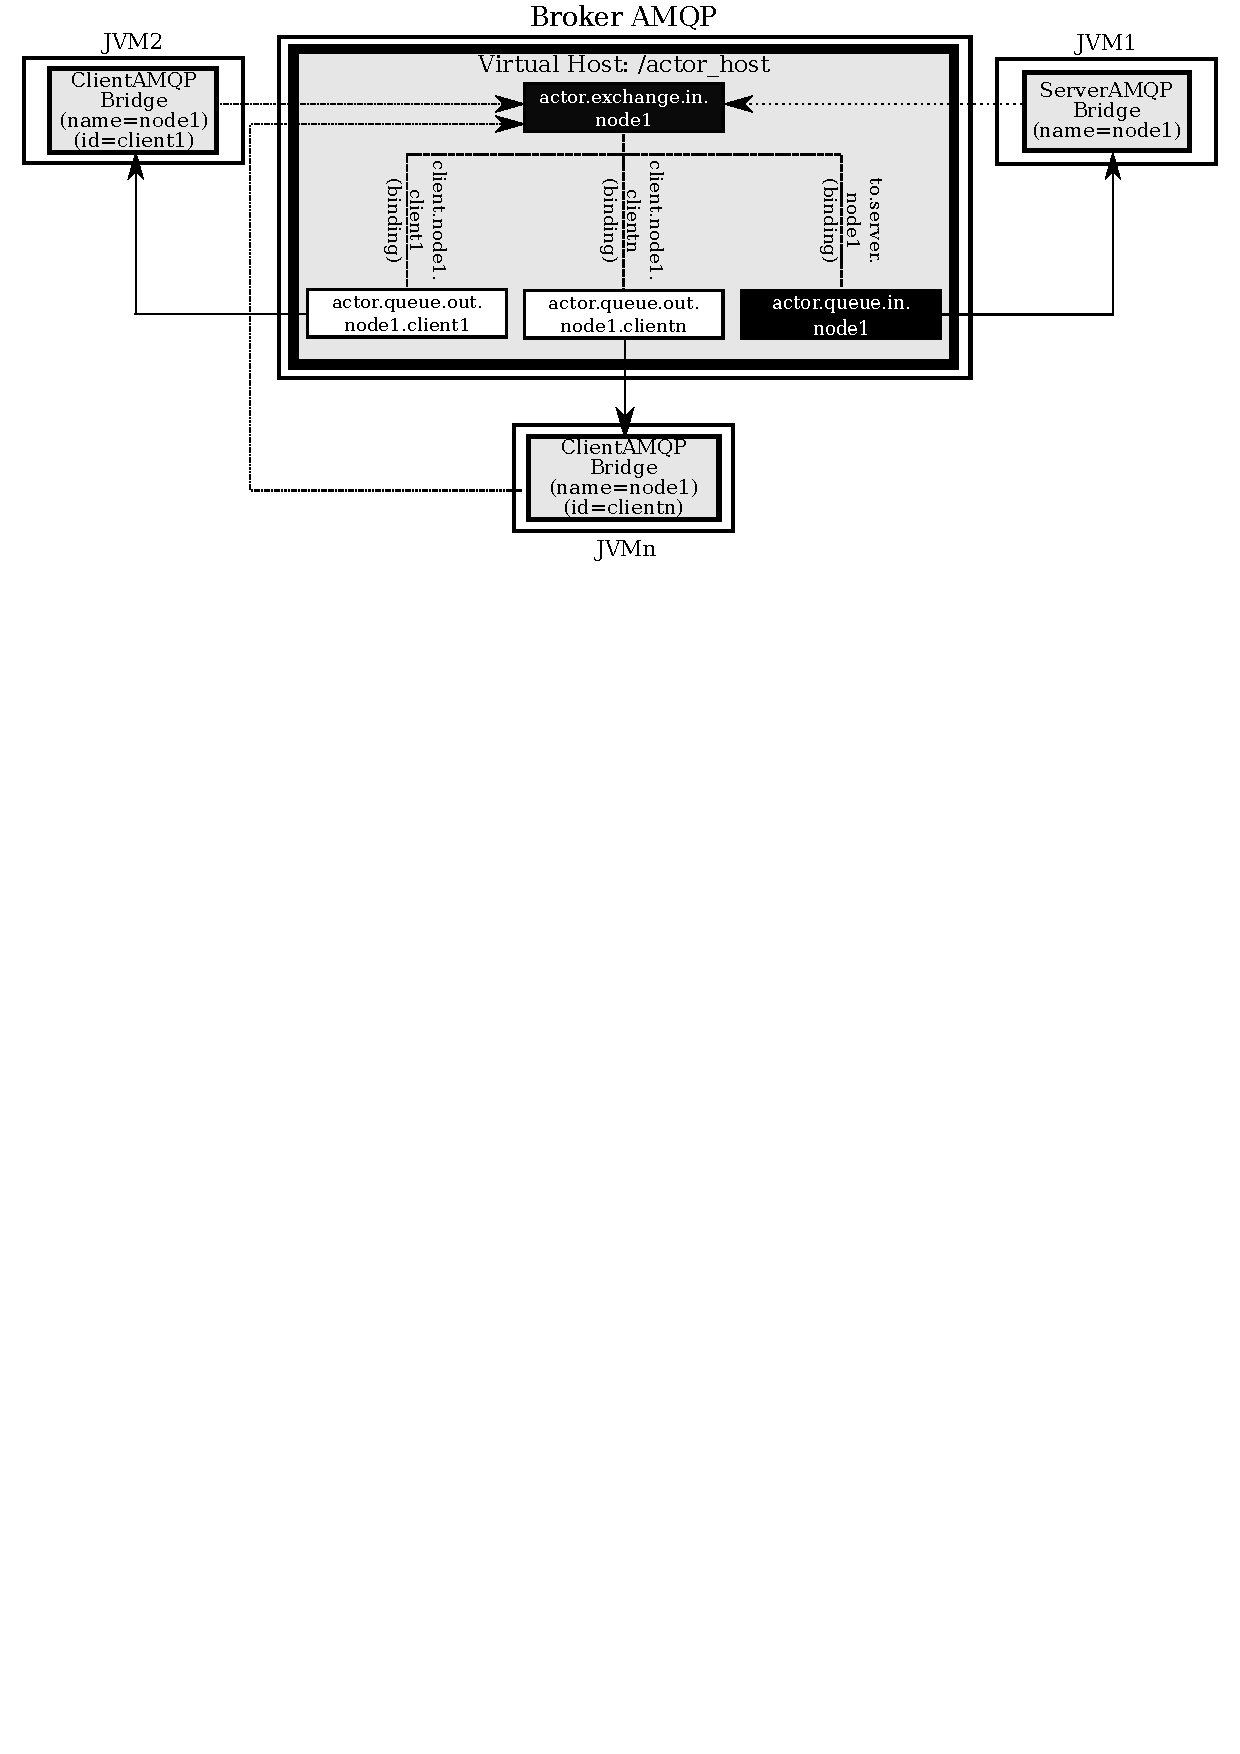
\includegraphics[scale=.50]{figuras/bridges-broker-all-together5.pdf}
		\end{figure}
 	}
}
\subsection{Integra\c{c}\~ao com o Akka}
\frame{\frametitle{Novos componentes}
	\only<1>{ 		
  		\begin{figure}[hbtp]
			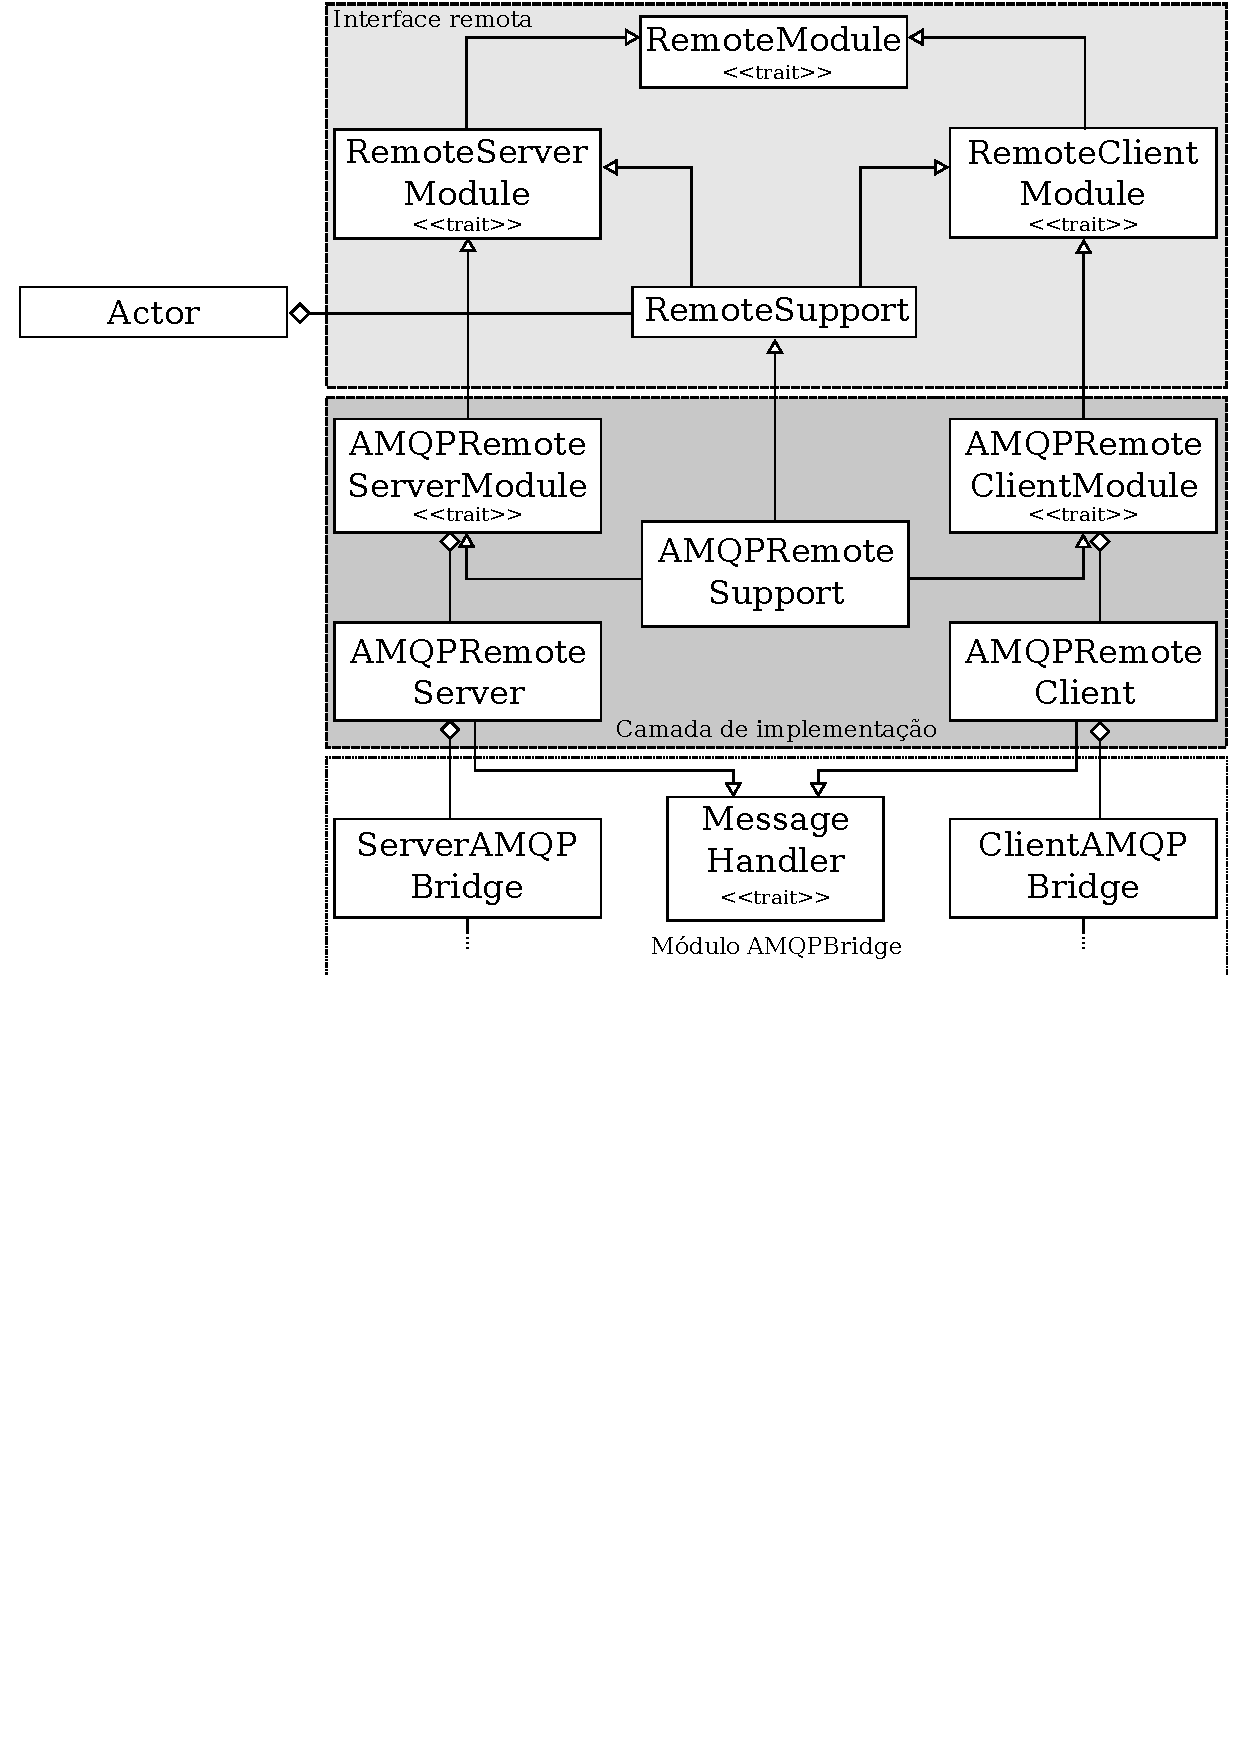
\includegraphics[scale=.35]{figuras/remote-actor-amqp-colaboracao.pdf}
		\end{figure}
 	}	
}
\frame{\frametitle{Adapta\c{c}\~oes e altera\c{c}\~oes necess\'arias}
	\only<1>{
 		\begin{enumerate}
			\item Adapta\c{c}\~ao dos valores para host e porta recebidos nos m\'etodos da biblioteca do Akka para o padr\~ao host@porta
			\item Novas entradas na se\c{c}\~ao remote do arquivo de configura\c{c}\~oes do Akka:
				\begin{itemize}
					\item Informa\c{c}\~oes para conex\~ao com o \textit{message broker}
					\item Pol\'iticas de armazemanto e compartilhamento de canais
					\item Identificador utilizado na cria\c{c}\~ao de pontes clientes
				\end{itemize}
			\item Novo campo no formato das mensagens (RemoteMessageProtocol) para que o servidor remoto possa identificar o cliente remetente
		\end{enumerate}
	}
}
\frame{\frametitle{Fluxo de envio de mensagens}
	\only<1>{ 		
	  		\begin{figure}[hbtp]
				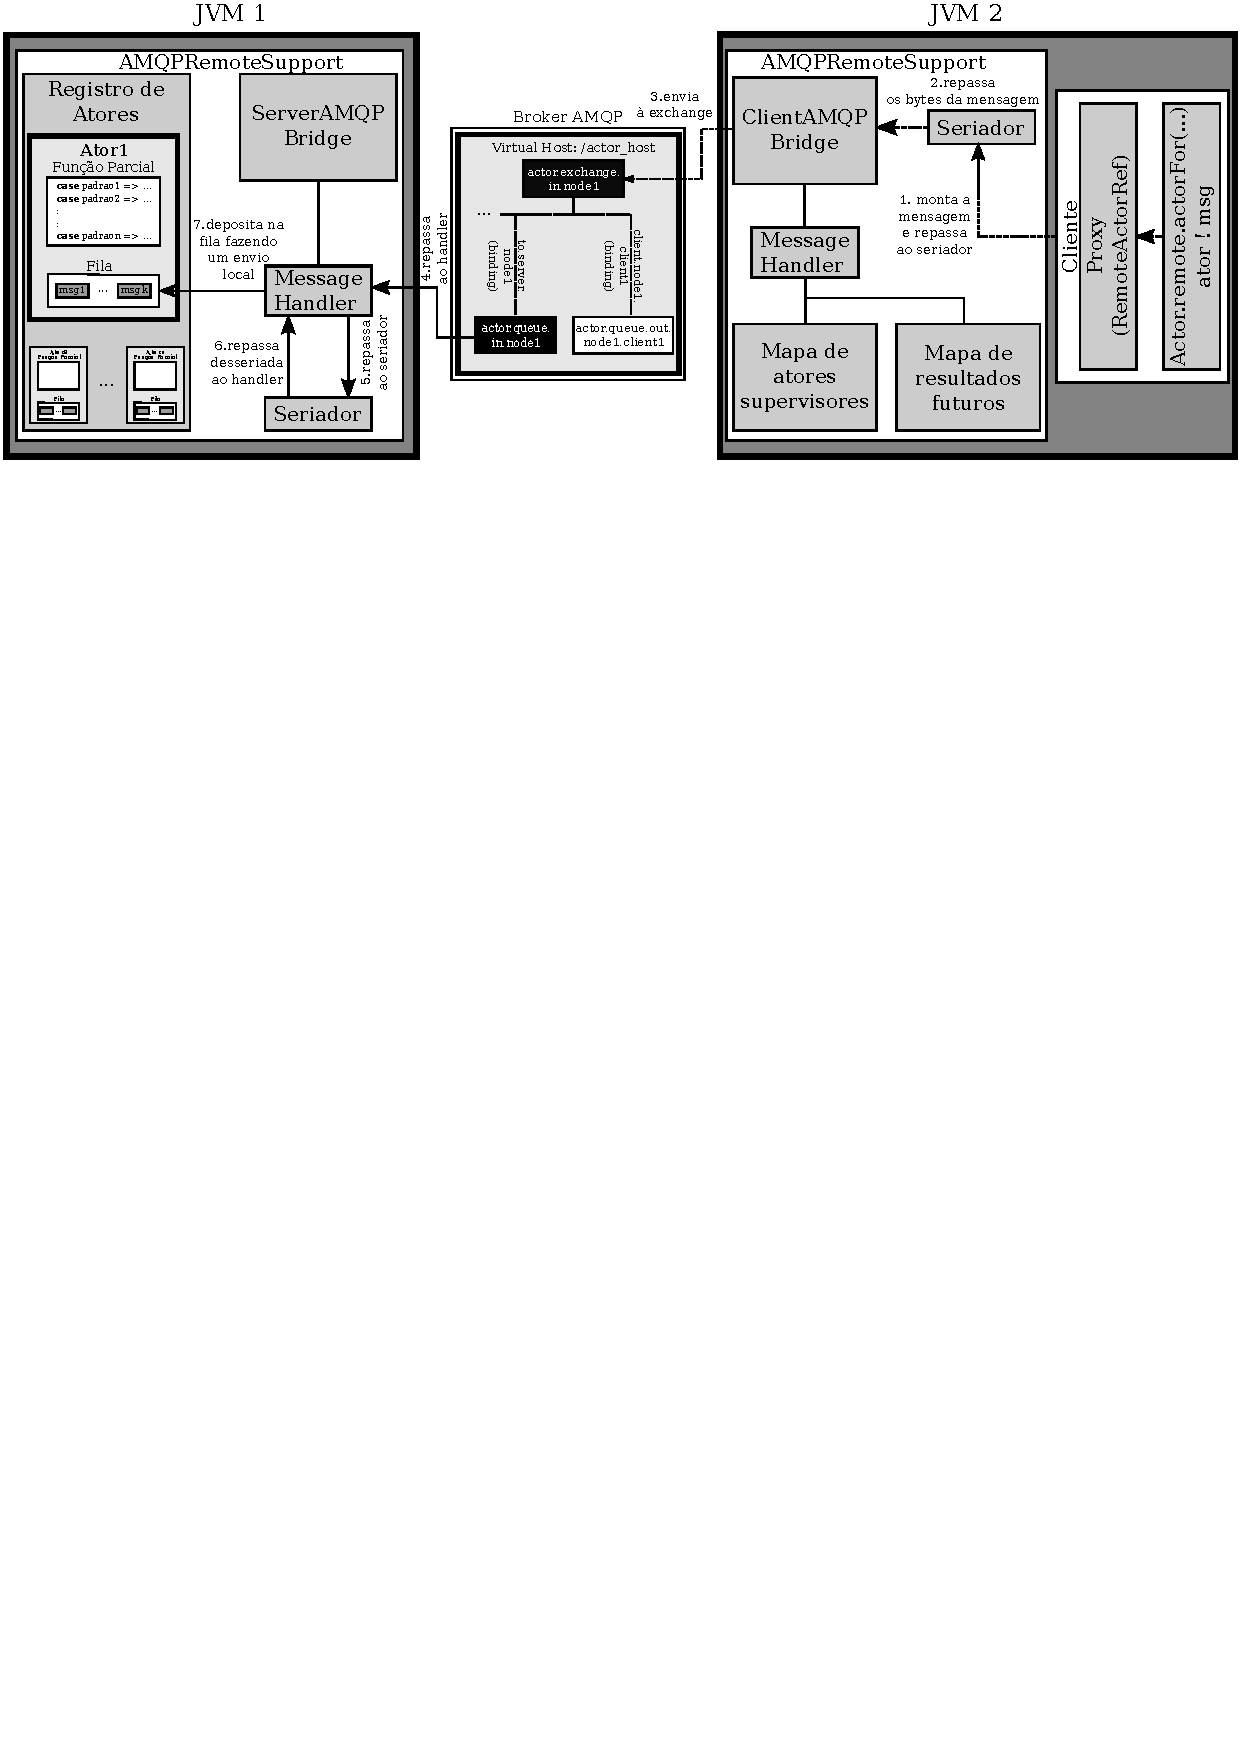
\includegraphics[scale=.55]{figuras/remote-actor-message-flow-amqp.pdf}
			\end{figure}
	 	}
	}

\section{Resultados experimentais} 
\subsection{Trading System}
\frame{\frametitle{Trading System}
	\begin{figure}[hbtp]
		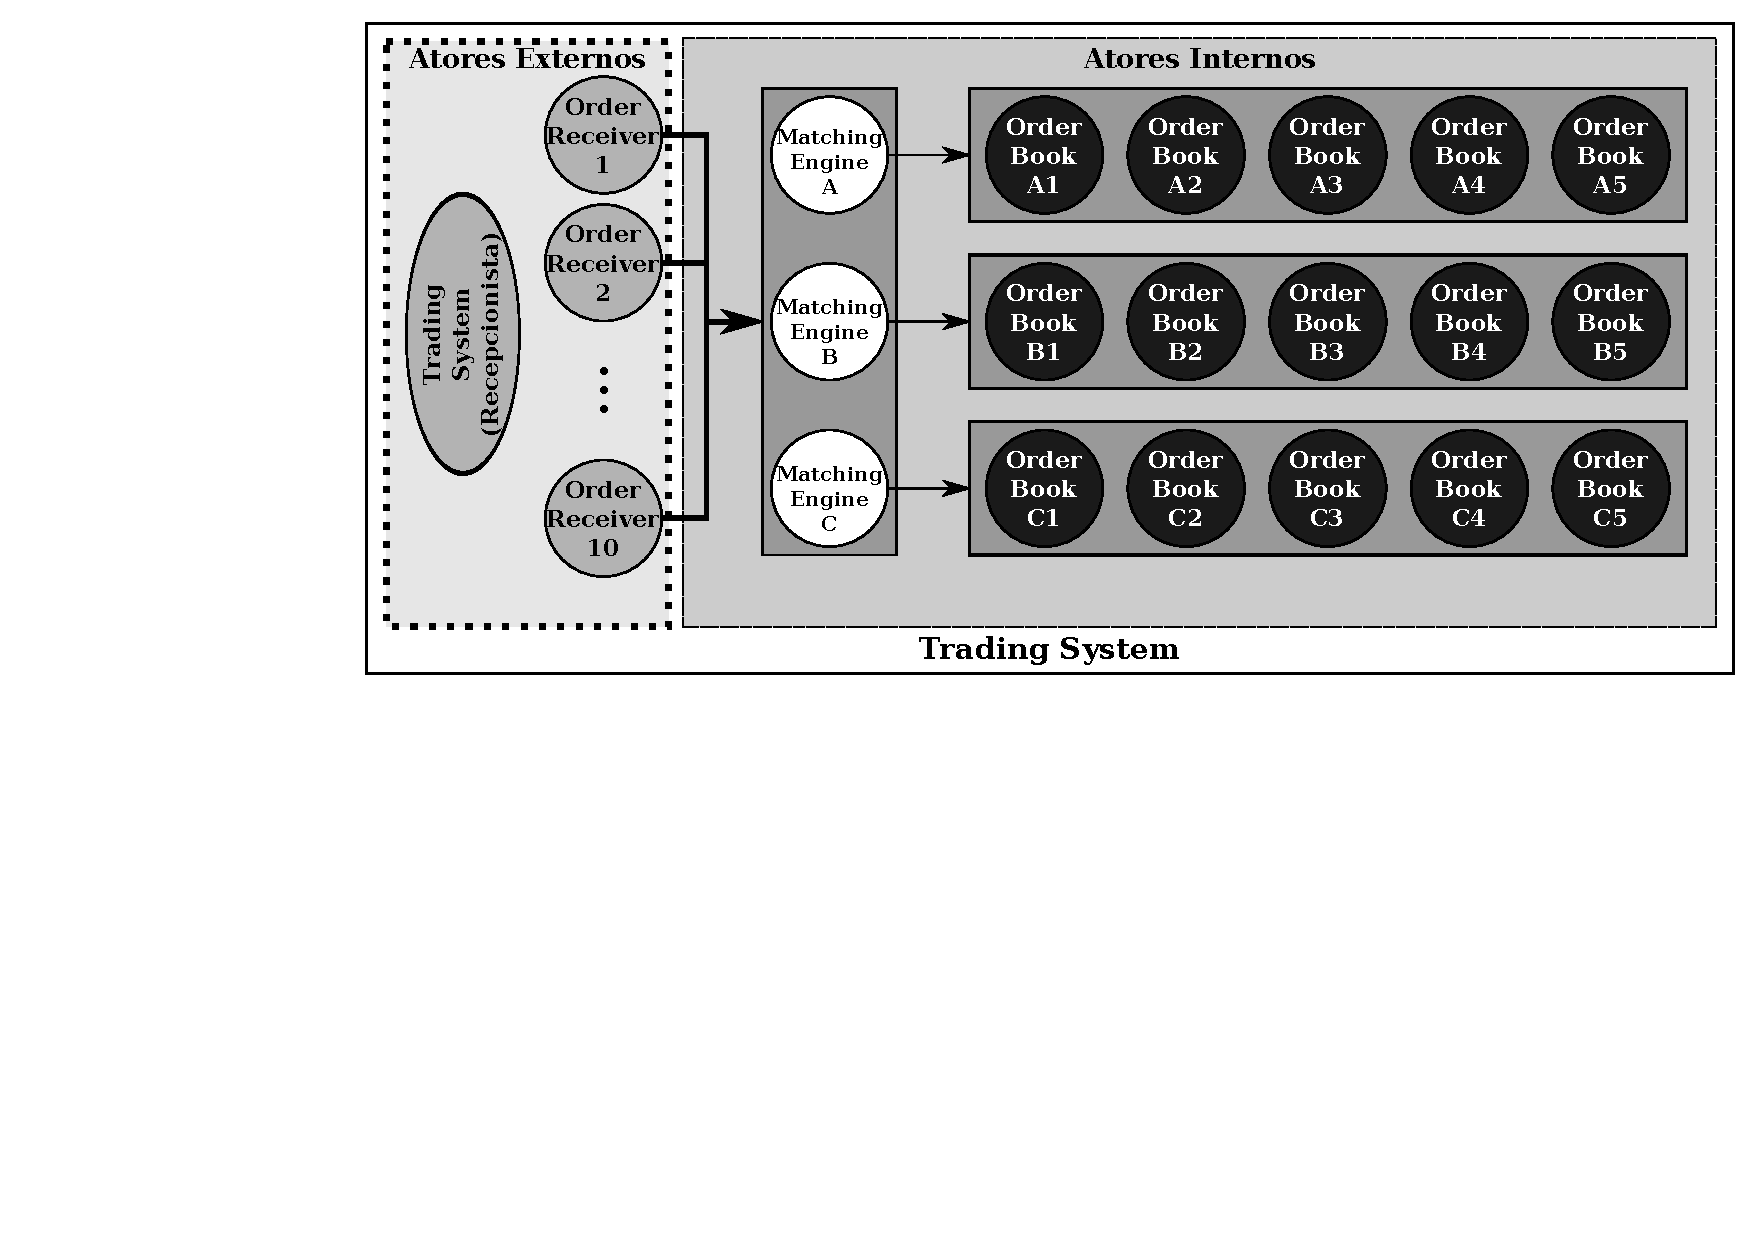
\includegraphics[scale=.4]{figuras/trading-system.pdf}
	\end{figure}
}
\subsection{Compara\c{c}\~ao de desempenho}
\frame{\frametitle{Rede de baixa lat\^encia}
	\only<1>{
		\begin{figure}[hbtp]
			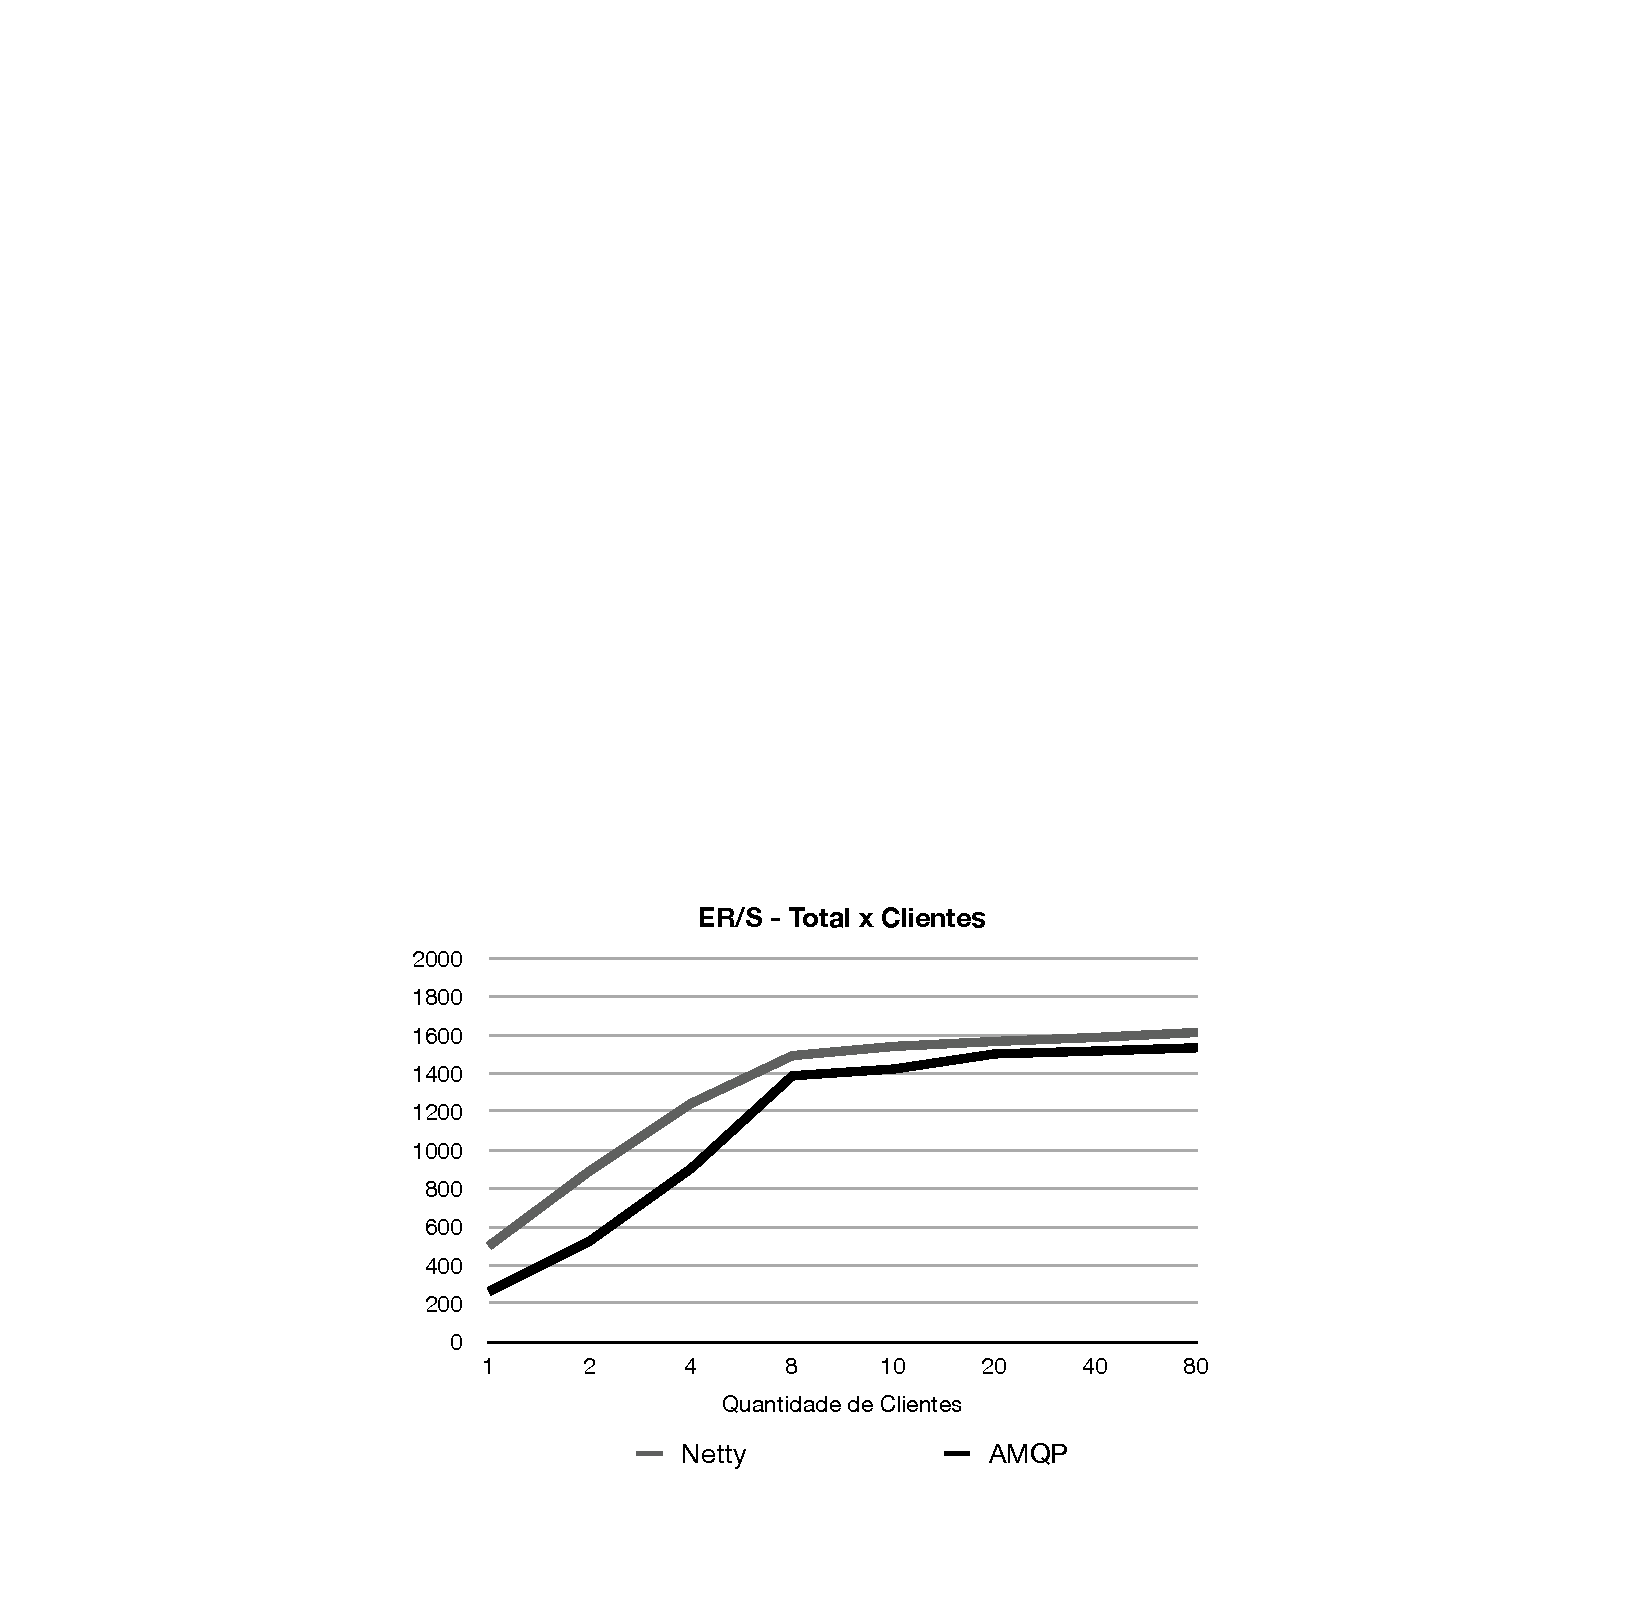
\includegraphics[scale=.5]{figuras/grafico-er.pdf}
		\end{figure}
	}
}

\frame{\frametitle{Rede de alta lat\^encia (wireless)}
	\only<1>{
		\begin{figure}[hbtp]
			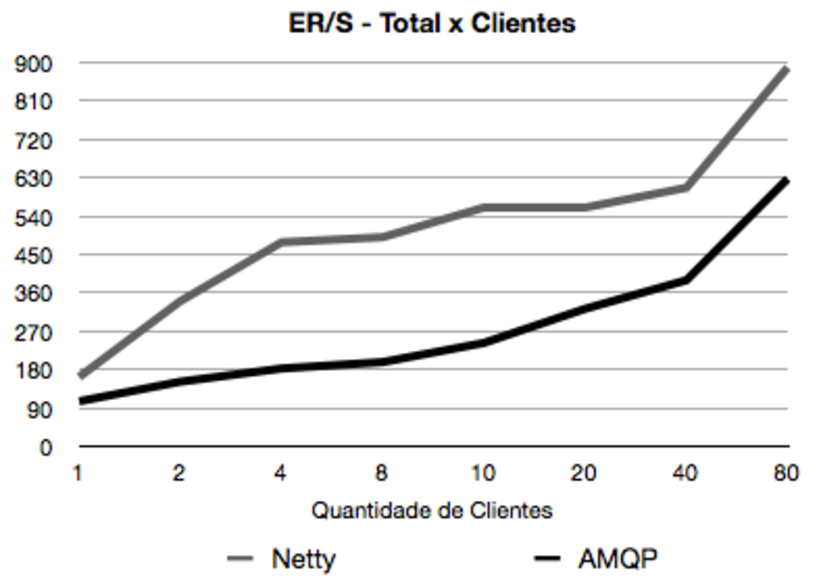
\includegraphics[scale=.5]{figuras/grafico-er-lento.pdf}
		\end{figure}
	}
}

\frame{\frametitle{Fluxo nas redes de alta e baixa lat\^encia}
	\only<1>{
		\begin{figure}[hbtp]
			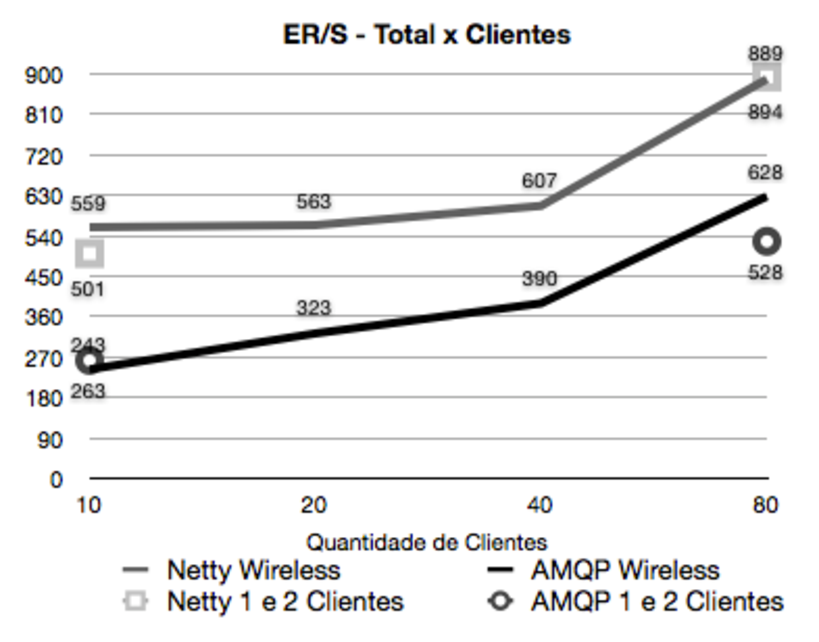
\includegraphics[scale=.5]{figuras/grafico-er-lento-e-normal.pdf}
		\end{figure}
	}
}

\section{Considera\c{c}\~oes finais e trabalhos futuros}
\subsection{Considera\c{c}\~oes finais}
\frame{\frametitle{Considera\c{c}\~oes finais}
 consideracoes finais
}
\subsection{Trabalhos futuros}
\frame{\frametitle{Trabalhos futuros}
	\begin{itemize}
		\item Melhoria no tratamento de erros nas pontes AMQP
			\begin{itemize}
				\item Aproveitar a hierarquia de supervis\~ao j\'a definida nas pontes AMQP para o tratamento de erros
				\item Implementar suporte a reconex\~ao e restaura\c{c}\~ao do estado dos atores relacionados a ponte AMQP no
				caso de desconex\~oes ou falhas de rede
			\end{itemize}
		\item Experimentos em um ambiente de computa\c{c}\~ao em nuvem
			\begin{itemize}
				\item Fazer as altera\c{c}\~oes necess\'arias para que nossa implementa\c{c}\~ao de atores remotos
				possa ser implantada em uma infraestrutura de computa\c{c}\~ao em nuvem
				\item Fazer uma avalia\c{c}\~ao experiemental do \textit{Trading System} na nuvem utilizando uma
				quantidade de clientes bem maiores do que as utilizadas em nossos experimentos
			\end{itemize}
	\end{itemize}
}

\frame{
 	\frametitle{Perguntas}
		\begin{figure}[hbtp]
			
\includegraphics[scale=0.3]{figuras/question.pdf}
		\end{figure}
 	}


\end{document}
